% !TEX options=--shell-escape

%!TEX root = ../my_thesis.tex

\documentclass[a4paper,11pt,fleqn,oneside]{book} % 'twoside' document for print, 'oneside' document for digital version

% boolean 'twosidedoc' contain true if the document is two-sided, false else
\usepackage{ifthen}
\newboolean{twosidedoc}
\makeatletter
%preamble
\if@twoside%
  \setboolean{twosidedoc}{true}
  % https://tex.stackexchange.com/questions/62572/twoside-introduces-incorrect-linespacing-at-end-of-section
  \raggedbottom % disable auto vertical spacing when two-sided doc
\else%
  \setboolean{twosidedoc}{false}
\fi%
\makeatother

\usepackage[bottom]{footmisc} % footnotes at the bottom of the page
\usepackage[T1]{fontenc}
\usepackage[utf8]{inputenc}
\usepackage[english,french]{babel}
\usepackage{eulervm}
\ifthenelse{\boolean{twosidedoc}}
{\usepackage[a4paper,top=25mm,bottom=25mm,left=30mm,right=20mm]{geometry}} % two-sided document (for print)
{\usepackage[a4paper,top=25mm,bottom=25mm,left=25mm,right=25mm]{geometry}} % one-sided document (digital version)
\usepackage{setspace} % increase interline spacing slightly
\usepackage{graphicx}
\usepackage[table]{xcolor}
\usepackage{booktabs}
\usepackage{lipsum}
\usepackage{microtype}
\usepackage{url}
\usepackage[final]{pdfpages}
\usepackage{fancyhdr}
\usepackage{tikz}
\usepackage[explicit]{titlesec}
\usepackage{amsmath}
\usepackage{amssymb}

\usepackage{color}

\definecolor{Comment}{RGB}{97,161,176}

\definecolor{btfGreen}{RGB}{51,160,44}
\definecolor{btfRed}{RGB}{190,60,90}

\definecolor{bleuUni}{RGB}{0, 157, 224}
\definecolor{marronUni}{RGB}{68, 58, 49}
\definecolor{grayMarronUni}{RGB}{60, 60, 60}
\definecolor{grayBleuUni}{RGB}{118, 118, 118}

\definecolor{bluecite}{HTML}{009DE0}

\definecolor{Paired-2}{RGB}{166,206,227}
\definecolor{Paired-1}{RGB}{31,120,180}
\definecolor{Paired-4}{RGB}{178,223,138}
\definecolor{Paired-3}{RGB}{51,160,44}
\definecolor{Paired-6}{RGB}{251,154,153}
\definecolor{Paired-5}{RGB}{227,26,28}
\definecolor{Paired-8}{RGB}{253,191,111}
\definecolor{Paired-7}{RGB}{255,127,0}
\definecolor{Paired-10}{RGB}{202,178,214}
\definecolor{Paired-9}{RGB}{106,61,154}
\definecolor{Paired-12}{RGB}{255,255,153}
\definecolor{Paired-11}{RGB}{177,89,40}
\definecolor{Accent-1}{RGB}{127,201,127}
\definecolor{Accent-2}{RGB}{190,174,212}
\definecolor{Accent-3}{RGB}{253,192,134}
\definecolor{Accent-4}{RGB}{255,255,153}
\definecolor{Accent-5}{RGB}{56,108,176}
\definecolor{Accent-6}{RGB}{240,2,127}
\definecolor{Accent-7}{RGB}{191,91,23}
\definecolor{Accent-8}{RGB}{102,102,102}
\definecolor{Spectral-1}{RGB}{158,1,66}
\definecolor{Spectral-2}{RGB}{213,62,79}
\definecolor{Spectral-3}{RGB}{244,109,67}
\definecolor{Spectral-4}{RGB}{253,174,97}
\definecolor{Spectral-5}{RGB}{254,224,139}
\definecolor{Spectral-6}{RGB}{255,255,191}
\definecolor{Spectral-7}{RGB}{230,245,152}
\definecolor{Spectral-8}{RGB}{171,221,164}
\definecolor{Spectral-9}{RGB}{102,194,165}
\definecolor{Spectral-10}{RGB}{50,136,189}
\definecolor{Spectral-11}{RGB}{94,79,162}
\definecolor{Set1-1}{RGB}{228,26,28}
\definecolor{Set1-2}{RGB}{55,126,184}
\definecolor{Set1-3}{RGB}{77,175,74}
\definecolor{Set1-4}{RGB}{152,78,163}
\definecolor{Set1-5}{RGB}{255,127,0}
\definecolor{Set1-6}{RGB}{255,255,51}
\definecolor{Set1-7}{RGB}{166,86,40}
\definecolor{Set1-8}{RGB}{247,129,191}
\definecolor{Set1-9}{RGB}{153,153,153}
\definecolor{Set2-1}{RGB}{102,194,165}
\definecolor{Set2-2}{RGB}{252,141,98}
\definecolor{Set2-3}{RGB}{141,160,203}
\definecolor{Set2-4}{RGB}{231,138,195}
\definecolor{Set2-5}{RGB}{166,216,84}
\definecolor{Set2-6}{RGB}{255,217,47}
\definecolor{Set2-7}{RGB}{229,196,148}
\definecolor{Set2-8}{RGB}{179,179,179}
\definecolor{Dark2-1}{RGB}{27,158,119}
\definecolor{Dark2-2}{RGB}{217,95,2}
\definecolor{Dark2-3}{RGB}{117,112,179}
\definecolor{Dark2-4}{RGB}{231,41,138}
\definecolor{Dark2-5}{RGB}{102,166,30}
\definecolor{Dark2-6}{RGB}{230,171,2}
\definecolor{Dark2-7}{RGB}{166,118,29}
\definecolor{Dark2-8}{RGB}{102,102,102}
\definecolor{Reds-1}{RGB}{255,245,240}
\definecolor{Reds-2}{RGB}{254,224,210}
\definecolor{Reds-3}{RGB}{252,187,161}
\definecolor{Reds-4}{RGB}{252,146,114}
\definecolor{Reds-5}{RGB}{251,106,74}
\definecolor{Reds-6}{RGB}{239,59,44}
\definecolor{Reds-7}{RGB}{203,24,29}
\definecolor{Reds-8}{RGB}{165,15,21}
\definecolor{Reds-9}{RGB}{103,0,13}
\definecolor{Greens-1}{RGB}{247,252,245}
\definecolor{Greens-2}{RGB}{229,245,224}
\definecolor{Greens-3}{RGB}{199,233,192}
\definecolor{Greens-4}{RGB}{161,217,155}
\definecolor{Greens-5}{RGB}{116,196,118}
\definecolor{Greens-6}{RGB}{65,171,93}
\definecolor{Greens-7}{RGB}{35,139,69}
\definecolor{Greens-8}{RGB}{0,109,44}
\definecolor{Greens-9}{RGB}{0,68,27}
\definecolor{Blues-1}{RGB}{247,251,255}
\definecolor{Blues-2}{RGB}{222,235,247}
\definecolor{Blues-3}{RGB}{198,219,239}
\definecolor{Blues-4}{RGB}{158,202,225}
\definecolor{Blues-5}{RGB}{107,174,214}
\definecolor{Blues-6}{RGB}{66,146,198}
\definecolor{Blues-7}{RGB}{33,113,181}
\definecolor{Blues-8}{RGB}{8,81,156}
\definecolor{Blues-9}{RGB}{8,48,107}
 % file containing all the colors definitions

\setstretch{1.05} % package 'setspace'
% \setlength{\parindent}{0pt} % do not indent paragraphs

\makeatletter
\renewcommand{\sectionmark}[1]{\markright{\thesection\ #1}}
\pagestyle{fancy}
  \fancyhf{}
  \renewcommand{\headrulewidth}{0.4pt}
%  \renewcommand{\headrule}{\hbox to\headwidth{%
%    \color{bleuUni}\leaders\hrule height \headrulewidth\hfill}}

\ifthenelse{\boolean{twosidedoc}}
{
\renewcommand{\headrule}{{\color{grayBleuUni}%
\hrule width\headwidth height\headrulewidth \vskip-\headrulewidth}}
}
{
\renewcommand{\headrule}{{\color{bleuUni}%
\hrule width\headwidth height\headrulewidth \vskip-\headrulewidth}}
}

\renewcommand{\footrulewidth}{0.0pt}
  \fancyhead[OR]{\bfseries \nouppercase{\rightmark}}
  \fancyhead[EL]{\bfseries \nouppercase{\leftmark}}
  \ifthenelse{\boolean{twosidedoc}}
  {\fancyfoot[EL,OR]{\thepage}}
  {\fancyfoot[EC,OC]{\thepage}}
\fancypagestyle{plain}{
  \fancyhf{}
  \renewcommand{\headrulewidth}{0pt}
  \renewcommand{\footrulewidth}{0pt}
  \ifthenelse{\boolean{twosidedoc}}
  {\fancyfoot[EL,OR]{\thepage}}
  {\fancyfoot[CO,CE]{\thepage}}
}
\fancypagestyle{addpagenumbersforpdfimports}{
  \fancyhead{}
  \renewcommand{\headrulewidth}{0pt}
  \fancyfoot{}
  \ifthenelse{\boolean{twosidedoc}}
  {\fancyfoot[RO,LE]{\thepage}}
  {\fancyfoot[CO,CE]{\thepage}}
}
\makeatother

\makeatletter
\def\cleardoublepage{\clearpage\if@twoside \ifodd\c@page\else
  \hbox{}
  \thispagestyle{empty}
  \newpage
  \if@twocolumn\hbox{}\newpage\fi\fi\fi}
\makeatother \clearpage{\pagestyle{plain}\cleardoublepage}

\newcommand*\cleartoleftpage{%
   \clearpage
   \ifodd\value{page}\hbox{}\vspace*{\fill}\thispagestyle{empty}\newpage\fi
}

%%%%% CHAPTER HEADER %%%%

\newcommand*\chapterlabel{}
%\renewcommand{\thechapter}{\Roman{chapter}}
\titleformat{\chapter}[display]  % type (section,chapter,etc...) to vary,  shape (eg display-type)
  {\normalfont\bfseries\Huge} % format of the chapter
  {\gdef\chapterlabel{\thechapter\ }}     % the label
  {0pt} % separation between label and chapter-title
    {
    \tikzset{external/export=false}
    \begin{tikzpicture}[remember picture,overlay]
    \node[yshift=-6cm] at (current page.north west)
      {\begin{tikzpicture}[remember picture, overlay]
        \ifthenelse{\boolean{twosidedoc}}
        {\draw[fill=bleuUni,bleuUni] (0,0) rectangle(28.5mm,15mm);}
        {\draw[fill=bleuUni,bleuUni] (0,0) rectangle(23.5mm,15mm);}
        \ifthenelse{\boolean{twosidedoc}}
        {\node[anchor=north east,yshift=-5.2cm,xshift=27mm,minimum height=30mm,inner sep=0mm] at (current page.north west)}
        {\node[anchor=north east,yshift=-5.2cm,xshift=22mm,minimum height=30mm,inner sep=0mm] at (current page.north west)}
        {\parbox[top][30mm][t]{15mm}{\raggedleft $\phantom{\textrm{l}}$\color{white}\chapterlabel}};  %the black l is just to get better base-line alingement
        \ifthenelse{\boolean{twosidedoc}}
        {\node[anchor=north west,yshift=-5.2cm,xshift=30mm,text width=\textwidth,minimum height=30mm,inner sep=0mm] at (current page.north west)}
        {\node[anchor=north west,yshift=-5.2cm,xshift=25mm,text width=\textwidth,minimum height=30mm,inner sep=0mm] at (current page.north west)}
        {\parbox[top][30mm][t]{\textwidth}{\color{black}#1}};
       \end{tikzpicture}
      };
   \end{tikzpicture}
   \gdef\chapterlabel{}
  } % code before the title body

\titlespacing*{\chapter}{0pt}{35pt}{20pt}
\titlespacing*{\section}{0pt}{13.2pt}{*0}  % 13.2pt is line spacing for a text with 11pt font size
\titlespacing*{\subsection}{0pt}{13.2pt}{*0}
\titlespacing*{\subsubsection}{0pt}{13.2pt}{*0}

% Fix the problem with delimiter size caused by fourier and amsmath packages.
\makeatletter
\def\resetMathstrut@{%
  \setbox\z@\hbox{%
    \mathchardef\@tempa\mathcode`\(\relax
      \def\@tempb##1"##2##3{\the\textfont"##3\char"}%
      \expandafter\@tempb\meaning\@tempa \relax
  }%
  \ht\Mathstrutbox@1.2\ht\z@ \dp\Mathstrutbox@1.2\dp\z@
}
\makeatother

%%%%%%%%%%%%%%%%%%%%%%%%%%%%%%%%%%%%%%%%%%%%%%
%
%		Thesis Settings
%		Custom settings
%
%		2011
%
%%%%%%%%%%%%%%%%%%%%%%%%%%%%%%%%%%%%%%%%%%%%%%

%
%   Use this file for your own custom packages, command-definitions, etc...
%

% Rubber configuration --------------------------------------------------------
% rubber: setlist arguments --shell-escape

% Packages --------------------------------------------------------------------
\usepackage[english]{minitoc} % rappel du plan du chapitre en cours
\usepackage{array}
\usepackage{longtable} % pour la liste des notations
\usepackage[toc,page]{appendix}
\usepackage{pgfplots} % package pour les graphiques
\usepackage[english,onelanguage,ruled,linesnumbered,vlined]{algorithm2e}
\usepackage{multibib}
\usepackage{multirow}
\usepackage{multicol}
\usepackage{xspace}
\usepackage{xcolor}
\usepackage{pifont}
\usepackage{hyperref}
\usepackage{minted} % beautiful source code
\usepackage{sourcecodepro} % beautiful source code
\usepackage{chngcntr}
\usepackage{bm} % bold math
\usepackage{geometry} % reduce margins
\usepackage{tkz-kiviat}
\usepackage{subfig}
\usepackage{adjustbox}

% Parameters ------------------------------------------------------------------
\setcounter{secnumdepth}{4} % package 'minitoc'
\setcounter{tocdepth}{3} % package 'minitoc'
\newcites{mine}{Publications} % package 'multibib'
\newlength{\Oldarrayrulewidth} % package 'array'
\setminted{fontsize=\small,framesep=2mm} % package 'minted'
\usemintedstyle{friendly} % package 'minted'
\counterwithin{listing}{chapter} % package 'chngcntr'
\usetikzlibrary{arrows} % package 'tikz'
\SetKwComment{Comment}{$\triangleright$\ }{} % package 'algorithm2e'

\newcolumntype{L}[1]{>{\raggedright\let\newline\\\arraybackslash\hspace{0pt}}m{#1}}
\newcolumntype{C}[1]{>{\centering\let\newline\\\arraybackslash\hspace{0pt}}m{#1}}
\newcolumntype{R}[1]{>{\raggedleft\let\newline\\\arraybackslash\hspace{0pt}}m{#1}}
\newlength{\simcolwidth}
\setlength{\simcolwidth}{0.5cm}

% Math operators --------------------------------------------------------------
\DeclareMathOperator{\card}{card}
\DeclareMathOperator{\diag}{diag}
\DeclareMathOperator{\prob}{P}
\DeclareMathOperator*{\maxstar}{max*}
\DeclareMathOperator*{\argmax}{arg\,max}
\DeclareMathOperator*{\decide}{decide}
\DeclareMathOperator*{\computeGamma}{computeGamma}
\DeclareMathOperator*{\computeAlpha}{computeAlpha}
\DeclareMathOperator*{\computeBeta}{computeBeta}
\DeclareMathOperator*{\computeExtrinsic}{computeExtrinsic}
\DeclareMathOperator*{\initAlpha}{initAlpha}
\DeclareMathOperator*{\initBeta}{initBeta}
\DeclareMathOperator*{\sizeof}{sizeof}
\DeclareMathOperator*{\argmin}{arg\,min}

% Commands --------------------------------------------------------------------
\newcommand{\R}{\textsuperscript{\textregistered}}
\newcommand{\TM}{\textsuperscript{\texttrademark}}
% \newcommand{\cmark}{\ding{51}}
% \newcommand{\xmark}{\ding{55}}
\definecolor{btfGreen}{RGB}{51,160,44}
\definecolor{btfRed}{RGB}{190,60,90}
\newcommand{\cmark}{\textcolor{btfGreen}{\ding{51}}}
\newcommand{\xmark}{\textcolor{btfRed}{\ding{55}}}
\newcommand{\AFFECT}{AFF3CT\xspace}
\newcommand{\MIPP}{\texttt{MIPP}\xspace}
\newcommand{\longMIPP}{\textsc{MyIntrinsics++}\xspace}
\newcommand{\TSIMD}{\texttt{T-SIMD}\xspace}
\newcommand{\xsimd}{\texttt{xsimd}\xspace}
\newcommand{\simdpp}{\texttt{simdpp}\xspace}
\newcommand{\Vc}{\texttt{Vc}\xspace}
\newcommand{\VCL}{\texttt{VCL}\xspace}
\newcommand{\BoostSIMD}{\texttt{Boost.SIMD}\xspace}
\newcommand{\bSIMD}{\texttt{bSIMD}\xspace}
\newcommand{\Cxx}{\texttt{C++}\xspace}
\newcommand{\Cxy}[1]{\texttt{C++{#1}}\xspace}
\newcommand{\CppUnit}{\texttt{CppUnit}\xspace}
\newcommand{\Cline}[2]{
  \noalign{\global\setlength{\Oldarrayrulewidth}{\arrayrulewidth}}
  \noalign{\global\setlength{\arrayrulewidth}{#1}}\cline{#2}
  \noalign{\global\setlength{\arrayrulewidth}{\Oldarrayrulewidth}}}
\renewcommand\listoflistingscaption{List of Source Codes}
\def\bl{big.\textsc{LITTLE}\xspace}
\def\big{big\xspace}
\def\little{\textsc{LITTLE}\xspace}
\def\odr{\textsc{Odroid}\xspace}
\def\odrx{\textsc{Odroid-XU+E}\xspace}
\def\juno{\textsc{Juno}\xspace}
\def\mus{\si{\micro\second}}

% Colors ----------------------------------------------------------------------
\definecolor{Paired-2}{RGB}{166,206,227}
\definecolor{Paired-1}{RGB}{31,120,180}
\definecolor{Paired-4}{RGB}{178,223,138}
\definecolor{Paired-3}{RGB}{51,160,44}
\definecolor{Paired-6}{RGB}{251,154,153}
\definecolor{Paired-5}{RGB}{227,26,28}
\definecolor{Paired-8}{RGB}{253,191,111}
\definecolor{Paired-7}{RGB}{255,127,0}
\definecolor{Paired-10}{RGB}{202,178,214}
\definecolor{Paired-9}{RGB}{106,61,154}
\definecolor{Paired-12}{RGB}{255,255,153}
\definecolor{Paired-11}{RGB}{177,89,40}
\definecolor{Accent-1}{RGB}{127,201,127}
\definecolor{Accent-2}{RGB}{190,174,212}
\definecolor{Accent-3}{RGB}{253,192,134}
\definecolor{Accent-4}{RGB}{255,255,153}
\definecolor{Accent-5}{RGB}{56,108,176}
\definecolor{Accent-6}{RGB}{240,2,127}
\definecolor{Accent-7}{RGB}{191,91,23}
\definecolor{Accent-8}{RGB}{102,102,102}
\definecolor{Spectral-1}{RGB}{158,1,66}
\definecolor{Spectral-2}{RGB}{213,62,79}
\definecolor{Spectral-3}{RGB}{244,109,67}
\definecolor{Spectral-4}{RGB}{253,174,97}
\definecolor{Spectral-5}{RGB}{254,224,139}
\definecolor{Spectral-6}{RGB}{255,255,191}
\definecolor{Spectral-7}{RGB}{230,245,152}
\definecolor{Spectral-8}{RGB}{171,221,164}
\definecolor{Spectral-9}{RGB}{102,194,165}
\definecolor{Spectral-10}{RGB}{50,136,189}
\definecolor{Spectral-11}{RGB}{94,79,162}
\definecolor{Set1-1}{RGB}{228,26,28}
\definecolor{Set1-2}{RGB}{55,126,184}
\definecolor{Set1-3}{RGB}{77,175,74}
\definecolor{Set1-4}{RGB}{152,78,163}
\definecolor{Set1-5}{RGB}{255,127,0}
\definecolor{Set1-6}{RGB}{255,255,51}
\definecolor{Set1-7}{RGB}{166,86,40}
\definecolor{Set1-8}{RGB}{247,129,191}
\definecolor{Set1-9}{RGB}{153,153,153}
\definecolor{Set2-1}{RGB}{102,194,165}
\definecolor{Set2-2}{RGB}{252,141,98}
\definecolor{Set2-3}{RGB}{141,160,203}
\definecolor{Set2-4}{RGB}{231,138,195}
\definecolor{Set2-5}{RGB}{166,216,84}
\definecolor{Set2-6}{RGB}{255,217,47}
\definecolor{Set2-7}{RGB}{229,196,148}
\definecolor{Set2-8}{RGB}{179,179,179}
\definecolor{Dark2-1}{RGB}{27,158,119}
\definecolor{Dark2-2}{RGB}{217,95,2}
\definecolor{Dark2-3}{RGB}{117,112,179}
\definecolor{Dark2-4}{RGB}{231,41,138}
\definecolor{Dark2-5}{RGB}{102,166,30}
\definecolor{Dark2-6}{RGB}{230,171,2}
\definecolor{Dark2-7}{RGB}{166,118,29}
\definecolor{Dark2-8}{RGB}{102,102,102}
\definecolor{Reds-1}{RGB}{255,245,240}
\definecolor{Reds-2}{RGB}{254,224,210}
\definecolor{Reds-3}{RGB}{252,187,161}
\definecolor{Reds-4}{RGB}{252,146,114}
\definecolor{Reds-5}{RGB}{251,106,74}
\definecolor{Reds-6}{RGB}{239,59,44}
\definecolor{Reds-7}{RGB}{203,24,29}
\definecolor{Reds-8}{RGB}{165,15,21}
\definecolor{Reds-9}{RGB}{103,0,13}
\definecolor{Greens-1}{RGB}{247,252,245}
\definecolor{Greens-2}{RGB}{229,245,224}
\definecolor{Greens-3}{RGB}{199,233,192}
\definecolor{Greens-4}{RGB}{161,217,155}
\definecolor{Greens-5}{RGB}{116,196,118}
\definecolor{Greens-6}{RGB}{65,171,93}
\definecolor{Greens-7}{RGB}{35,139,69}
\definecolor{Greens-8}{RGB}{0,109,44}
\definecolor{Greens-9}{RGB}{0,68,27}
\definecolor{Blues-1}{RGB}{247,251,255}
\definecolor{Blues-2}{RGB}{222,235,247}
\definecolor{Blues-3}{RGB}{198,219,239}
\definecolor{Blues-4}{RGB}{158,202,225}
\definecolor{Blues-5}{RGB}{107,174,214}
\definecolor{Blues-6}{RGB}{66,146,198}
\definecolor{Blues-7}{RGB}{33,113,181}
\definecolor{Blues-8}{RGB}{8,81,156}
\definecolor{Blues-9}{RGB}{8,48,107}
\definecolor{main-color}{rgb}{0.6627, 0.7176, 0.7764}
\definecolor{back-color}{rgb}{0.1686, 0.1686, 0.1686}
\definecolor{string-color}{rgb}{0.3333, 0.5254, 0.345}
\definecolor{key-color}{rgb}{0.8, 0.47, 0.196}
\definecolor{comment-color}{rgb}{0.35, 0.35, 0.35}
  % place your custom packages, etc... in this file!

%%%%%%%%%%%%%%%%%%%%%%%%%%%%%%%%%%%%%%%%%%%%%%
%%%%% HEAD: Book-Begin
%%%%%%%%%%%%%%%%%%%%%%%%%%%%%%%%%%%%%%%%%%%%%%
\begin{document}
\frontmatter
\begin{titlepage}

\includepdf[pages={1}]{head/titlepage}
\end{titlepage}
\selectlanguage{french}
\thispagestyle{empty}

\vspace*{\fill}

\begin{center}
	Thèse réalisée au  \\
	\vspace*{2em}
	Laboratoire de l'\bsc{Intégration du Matériau au Système} (IMS)\\
	de Bordeaux, au sein de l'équipe \bsc{CSN} du groupe \bsc{Conception}.\\
	\vspace*{1em}
	Université de Bordeaux, Laboratoire IMS\\
	UMR 5218 CNRS - Bordeaux INP\\
	351 Cours de la Libération\\
	Bâtiment A31\\
	33405 Talence Cedex\\
	FRANCE\\
	\vspace*{2em}

	Thèse réalisée au sein de l'entreprise\\
	\vspace*{2em}
	\bsc{EMG2}\\
	\vspace*{1em}
	EMG2\\
	15 Avenue de Norvège\\
	91140 Villebon-Sur-Yvette\\
	FRANCE\\
	\vspace*{2em}

\end{center}
% \cleardoublepage
\thispagestyle{empty}

\vspace*{\fill}

\begin{raggedleft}
A mes parents, à ma compagne.\\
\end{raggedleft}
\vspace*{\fill}


\setcounter{page}{1}
% \setlength{\parskip}{1em}
%!TEX root = ../my_thesis.tex

\cleardoublepage
\phantomsection
\chapter*{Résumé}
\markboth{Abstracts}{Abstracts}
\addcontentsline{toc}{chapter}{Abstracts}

\emph{Mots clefs :} kw1, kw2



\selectlanguage{english}
%!TEX root = ../my_thesis.tex

\cleardoublepage
\chapter*{Abstract}
\vskip1em

% Since their introduction in the 90's, turbo codes are considered as one of the
% most powerful error-correcting code. Thanks to their excellent trade-off between
% computational complexity and decoding performance, they were chosen in many
% communication standards.

% One way to characterize error-correcting codes is the evolution of the bit error
% rate as a function of signal-to-noise ratio (SNR). The turbo code error rate
% performance is divided in two different regions: the waterfall region and the
% error floor region. In the waterfall region, a slight increase in SNR results in
% a significant drop in error rate. In the error floor region, the error rate
% performance is only slightly improved as the SNR grows. This error floor can
% prevent turbo codes from being used in applications with low error rates
% requirements. Therefore various constructions optimizations that lower the error
% floor of turbo codes has been proposed in recent years by scientific community.
% However, these approaches can not be considered for already standardized turbo
% codes.

% This thesis addresses the problem of lowering the error floor of turbo codes
% without allowing any modification of the digital communication chain at the
% transmitter side. For this purpose, the state-of-the-art post-processing
% decoding method for turbo codes is detailed. It appears that efficient solutions
% are expensive to implement due to the required multiplication of computational
% resources or can strongly impact the overall decoding latency.

% Firstly, two decoding algorithms based on the monitoring of decoder's internal
% metrics are proposed. The waterfall region is enhanced by the first algorithm.
% However, the second one marginally lowers the error floor. Then, the study shows
% that in the error floor region, frames decoded by the turbo decoder are really
% close to the word originally transmitted. This is demonstrated by a proposition
% of an analytical prediction of the distribution of the number of bits in errors
% per erroneous frame. This prediction rests on the distance spectrum of turbo
% codes. Since the appearance of error floor region is due to only few bits in
% errors, an identification metric is proposed. This lead to the proposal of an
% algorithm that can correct residual errors. This algorithm, called
% Flip-and-Check, rests on the generation of candidate words, followed by
% verification according to an error-detecting code. Thanks to this decoding
% algorithm, the error floor of turbo codes encountered in different standards
% (LTE, CCSDS, DVB-RCS and DVB-RCS2) is lowered by one order of magnitude. This
% performance improvement is obtained without considering an important
% computational complexity overhead.

% Finally, a hardware decoding architecture implementing the Flip-and-Check
% algorithm is presented. A preliminary study of the impact of the different
% parameters of this algorithm is carried out. It leads to the definition of
% optimal values for some of these parameters. Others has to be adapted according
% to the gains targeted in terms of decoding performance. The possible integration
% of this algorithm along with existing turbo decoders is demonstrated thanks to
% this hardware architecture. This therefore enables the lowering of the error
% floors of standardized turbo codes.

\vskip0.5cm
\emph{Keywords:} Software-Defined Radio, Simulation, Error Correcting Codes,
                 Software Implementation, Optimization, Parallelization,
                 Open Source Code

\selectlanguage{french}
%!TEX root = ../my_thesis.tex

\cleardoublepage
\phantomsection
\chapter*{Résumé étendu}
\markboth{Extended Abstract in French}{Résumé étendu (\emph{Extended Abstract in French})}
\addcontentsline{toc}{chapter}{Extended Abstract in French}
\vskip1em

\newcommand{\vskipSectionResume}{\vskip0.5em}
\newcommand{\vskipSSSectionResume}{\vskip0.25em}

\section*{Chapitre~\ref{chap:ctx} - Contexte et objectifs}
\vskipSectionResume

\subsubsection*{Organisation}
\vskipSSSectionResume

Ce chapitre présente le contexte des systèmes de communication numérique. Il a
pour but de définir les notions qui seront réutilisées dans le manuscrit et de
donner une vue globale. Il définit aussi les principaux objectifs de cette
thèse.

La première partie présente le principe des systèmes de communication numérique
avec ses différentes composantes : l'émetteur, le canal et le récepteur. Les
métriques les plus couramment utilisées dans les communications numériques sont
présentées avec notamment la définition du taux d'erreur binaire (\emph{Bit
Error Rate}, BER) et du taux d'erreur trame (\emph{Frame Error Rate}, FER). La
deuxième partie détaille le modèle de canal par ajout de bruit blanc gaussien
(\emph{Additive White Gaussian Noise}, AWGN) et la modulation numérique binaire
par changement de phase (\emph{Binary Phase-Shift Keying}, BPSK) utilisées tout
au long du manuscrit. Une caractérisation du rapport signal sur bruit
(\emph{Signal-to-Noise Ratio}, SNR) est donnée ainsi que la notion de
probabilité à la sortie du canal et du démodulateur. La troisième partie
présente les familles de code correcteur d'erreurs considérées dans ce
manuscrit : à savoir les codes LDPC, les codes polaires et les turbo-codes. Les
traitements de codage (situé dans l’émetteur) et de décodage (situé dans le
récepteur) correspondants sont détaillés pour chaque famille de code. Ces
familles de code sont utilisées dans la plupart des standards actuels et
viennent avec une complexité calculatoire élevée. Par conséquent, ce sont de
bons candidats d'étude. Dans la dernière partie, deux contextes applicatifs
majeurs sont détaillés pour les familles de code considérées. La simulation
fonctionnelle permet la conception et la validation d'un schéma de codage. La
radio logicielle (\emph{Software-Defined Radio}, SDR) est un système de
communication radio où tous les composants sont implémentés en logiciel (par
opposition à des implémentations matérielles plus couramment utilisées).

\subsubsection*{Objectifs de la thèse}
\vskipSSSectionResume

À l'aube de la cinquième génération des standards pour la téléphonie mobile
(5G), le défi consiste maintenant à concevoir des systèmes de communication
capables de transmettre d'énormes quantités de données en peu de temps, à un
faible coût énergétique et dans des environnements très variés. Les chercheurs
s'efforcent d'affiner encore les schémas de codage existants, afin d'obtenir de
faibles taux d'erreur résiduels grâce à des processus de décodage rapides,
souples et les moins complexes possible.

\paragraph{Simulation fonctionnelle}

La validation d'un système de codage nécessite d'estimer son taux d'erreur. En
général, il n'existe pas de modèle mathématique simple pour décrire ces
performances. La seule solution pratique consiste à effectuer une simulation
Monte Carlo de l'ensemble de la chaîne. Cela signifie que certaines données sont
générées, encodées, modulées, bruitées, décodées de manière aléatoire, et que
les performances sont ensuite estimées en mesurant le taux d'erreur binaire
(BER) et le taux d'erreur trame (FER) à la fin de la chaîne de communication
(après avis du décodeur). Ce processus a l'avantage d'être universel mais il
entraîne également trois problèmes principaux :

\begin{enumerate}
  \item \textbf{Temps de simulation :}
    $\sim 100$ trames erronées doivent être simulées pour estimer avec précision
    les BER/FER. Ainsi, la mesure d'un FER de $10^{-7}$ nécessite la simulation
    de la transmission de $\sim100\times 10^7=10^9$ trames. En supposant une
    trame de 1000~bits, le simulateur doit alors calculer la transmission de
    $10^{12}$~bits. En gardant à l'esprit que la complexité de calcul de
    l'algorithme de décodage peut être importante, plusieurs semaines ou mois
    peuvent être nécessaires pour estimer avec précision les BER/FER d'un schéma
    de codage (en particulier si le taux d'erreur est faible).

  \item \textbf{Hétérogénéité algorithmique :}
    un grand nombre de codes correcteurs d'erreurs ont été conçus au fil des
    années. Pour chaque famille de code, plusieurs configurations de décodage
    sont possibles. Si il est simple de décrire un schéma de codage unique, il
    est  plus difficile d'avoir une description logicielle unifiée qui prenne en
    charge tous les schémas de codage et les algorithmes associés. Cette
    difficulté provient de l'hétérogénéité des structures de données nécessaires
    pour décrire les différents schémas de codage canal : les turbo-codes sont
    basés sur des treillis, les codes LDPC sont bien définis sur des graphes
    bipartis et les codes polaires sont décodés efficacement à l'aide d'arbres
    binaires.

  \item \textbf{Reproductibilité :}
    il est généralement fastidieux de reproduire des résultats issus de la
    littérature. Cela peut s'expliquer par la grande quantité de paramètres
    empiriques nécessaires pour définir un système de communication, et par le
    fait que tous ne sont pas toujours rapportés dans les publications. En
    outre, le code source des simulateurs est rarement accessible au public.
    Par conséquent, beaucoup de temps est passé à ``réinventer la roue'' juste
    pour pouvoir comparer de nouveaux résultats avec l'état de l'art.
\end{enumerate}

\paragraph{Radio logicielle}

Le paradigme de la radio logicielle (\emph{Software-Defined Radio}, SDR) est
désormais considéré pour des systèmes de communication numérique réels. Pour
répondre aux contraintes posées par les systèmes temps réel, voici les
principaux défis à relever :

\begin{enumerate}
  \item \textbf{Haut débit :}
    les nouvelles applications comme le \emph{streaming} vidéo, peuvent être
    très gourmandes en données. Par conséquent, les tâches de calcul intensif de
    l'émetteur et du récepteur doivent être bien optimisées pour atteindre des
    niveaux de performance comparables aux implémentation matérielles.

  \item \textbf{Faible latence :}
    atteindre un débit élevé n'est pas toujours la contrainte majeure, par
    exemple, dans les applications d'audio-conférence, il est inconfortable de
    percevoir un retard lorsque les gens parlent.

  \item \textbf{Flexibilité :}
    les implémentations logicielles doivent pouvoir s'adapter à diverses
    configurations. Par exemple, lorsque le rapport signal sur bruit (SNR)
    change, le décodeur doit être capable se s'adapter ``à la volée'' à de
    nouveaux taux de codage.

  \item \textbf{Portabilité :}
    les solutions proposées peuvent être déployées sur des serveurs haut de
    gamme ainsi que dans des systèmes embarqués à faible consommation
    énergétique. De plus, de nombreux systèmes d'exploitation coexistent, et il
    est important de pouvoir supporter les plus communs comme Windows, macOS et
    Linux.
\end{enumerate}

\section*{Chapitre~\ref{chap:opt} - Stratégies d'optimisation}
\vskipSectionResume

\subsubsection*{Organisation}
\vskipSSSectionResume

Ce chapitre se concentre sur les stratégies d'optimisation dédiées aux
algorithmes de communication numérique. Nos contributions sont divisées en deux
parties : 1) les stratégies génériques et 2) les optimisations spécifiques.
La première partie décrit les stratégies génériques que nous avons proposées
pour optimiser les algorithmes présents dans les récepteurs de systèmes de
communication numérique. Il s'avère que la vectorisation est une des clefs pour
implémenter des solutions logicielles efficaces. Une bibliothèque dédiée ainsi
que des niveaux de parallélisme génériques sont proposés. La seconde partie est
consacrée à l'implémentation logicielle efficace d'un sous-ensemble
représentatif de décodeurs pour les trois grandes familles de code abordées plus
tôt, à savoir : les codes LDPC, les codes polaires et les turbo-codes.

\subsubsection*{Principaux résultats}
\vskipSSSectionResume

En premier lieu, des stratégies génériques pour l'implémentation efficace
d'algorithmes sur processeurs généralistes (CPUs) sont présentées. Une
contribution principale de ce chapitre est la proposition de \MIPP : une
bibliothèque qui encapsule les instructions vectorielles. L'idée est d'abstraire
les types de données et les multiples jeux d’instructions vectoriels existants
afin de proposer des implémentations logicielles ``universelles'' et efficaces
des algorithmes présents dans les récepteurs de systèmes de communication
numérique. Nous montrons que \MIPP n'introduit presque pas de surcoût par
rapport aux fonctions intrinsèques (ou du code assembleur). \MIPP fonctionne
aussi bien sur des représentations en virgule flottante et que sur des
représentations en virgule fixe. Pour les algorithmes présents dans les
récepteurs de systèmes de communication numérique, les représentations en
virgule fixe sont très intéressantes car elles permettent de traiter un plus
grand nombre d'éléments dans les registres vectoriels, avec un impact modéré sur
les performances de décodage. Pour résumer, \textbf{\MIPP améliore la
flexibilité et la portabilité du code source tout en conservant le même niveau
de performance.} Notez que la bibliothèque \MIPP a été valorisée suite à une
publication dans une conférence scientifique~\cite{Cassagne2018}.

Dans une deuxième partie, deux grandes stratégies de vectorisation sont
explicitement définies et présentées. La stratégie intra-trame fonctionne
sur une seule trame en s'appuyant sur le parallélisme inhérent à l'algorithme,
tandis que la stratégie inter-trames fonctionne sur plusieurs trames en
même temps. La stratégie intra-trame peut à la fois augmenter le débit et
diminuer la latence. Au contraire, la stratégie inter-trames n'améliore pas la
latence, mais elle s'accompagne d'une efficacité vectorielle potentiellement
plus élevée et peut conduire à des débits très élevés. Ces deux stratégies
peuvent être appliquées à tous les blocs de traitement des chaînes de
communication numérique. \textbf{Les stratégies intra-trame et inter-trames
constituent donc un point clé pour résoudre le problème de l'hétérogénéité
algorithmique.}

Les dernières parties du chapitre se concentrent sur la conception
d'implémentations logicielles efficaces des algorithmes de décodage présentés
dans le chapitre précédent. Les décodeurs LDPC, les décodeurs polaires et le
turbo-décodeur sont compatibles avec la stratégie inter-trames, tandis que les
décodeurs polaires sont aussi compatibles avec la stratégie intra-trame. En
fonction des familles de codes, nous nous concentrons sur différentes
contraintes. \textbf{Les décodeurs LDPC ont été mis en œuvre pour prendre en
charge de nombreuses variantes et donc pour maximiser la flexibilité} au prix de
débits plus faibles et de latences plus élevées par rapport à d'autres travaux.
Ce choix permet d'évaluer les performances de décodage de nombreuses
combinaisons algorithmiques. \textbf{Dans les décodeurs polaires, la flexibilité
ainsi que des optimisations agressives sont considérées et comparées. Ces
dernières permettent d'atteindre de très faibles latences.} \textbf{Enfin, le
turbo-décodeur se concentre sur l'obtention de débits les plus élevés possibles}
et certaines spécialisations sont faites pour la norme LTE. Il est à noter que
la plupart des implémentations logicielles proposées ont fait l'objet de
publications dans des conférences et des revues
scientifiques~\cite{Ghaffari2019,Leonardon2019,Cassagne2015c,Cassagne2016b,
Cassagne2016a}.

\section*{Chapitre~\ref{chap:aff3ct} - AFF3CT : une boîte à outils pour le codage canal}
\vskipSectionResume

\subsubsection*{Organisation}
\vskipSSSectionResume

Ce chapitre est consacré à la présentation de notre boîte à outils
\emph{open-source} nommée \AFFECT. La première partie décrit les principaux
prérequis en fonction de quatre objectifs : l'implémentation d'un logiciel
hautement performant, la prise en charge de l'hétérogénéité algorithmique, la
portabilité et la reproductibilité. Dans la deuxième partie, \AFFECT est comparé
aux autres bibliothèques logicielles de codage canal \verb|C|/\Cxx existantes.
La troisième partie présente \AFFECT comme une bibliothèque dédiée aux
algorithmes de communication numérique. L'architecture et les fonctionnalités du
logiciel sont décrites. Ensuite, des exemples d'utilisation de la bibliothèque
sont donnés en \Cxx et en MATLAB\R. La quatrième partie se concentre sur le
simulateur \AFFECT qui est livré dans la boîte à outils. Un aperçu des
explorations possibles est donné et notre comparateur de BER/FER est présenté. À
la fin, la stratégie de test d'\AFFECT est expliquée. Une dernière partie est
consacrée à l'impact d'\AFFECT dans les contextes industriels et universitaires.
Une revue des publications scientifiques qui ont utilisé \AFFECT est donnée.

\subsubsection*{Principaux résultats}
\vskipSSSectionResume

Tout d'abord, l'accent est mis sur \textbf{la bibliothèque \AFFECT qui vient
avec une architecture logicielle qui permet l'hétérogénéité algorithmique}. De
nombreuses familles de code correcteur d'erreurs sont supportées comme les
codes LDPC, les codes polaires, les turbo-codes, les turbo-codes produit, les
codes convolutifs, les codes BCH, les codes RS, etc. \textbf{À notre
connaissance, \AFFECT est la bibliothèque qui offre le support le plus complet
pour les algorithmes de codage canal.} \AFFECT est également livré avec de
multiples modèles de canaux  (AWGN, Rayleigh, BEC, BSC, etc.) et différents
schémas de modulation (PSK, QAM, PAM, OOK, CPM, SCMA, etc.). Toutes ces
implémentations efficaces d'algorithmes peuvent être utilisées à partir
d'interfaces. Des exemples d'utilisation de la bibliothèque sont donnés en \Cxx
natif ou en utilisant l'encapsulation MATLAB\R. La boîte à outils \AFFECT a fait
l'objet de publications dans une conférence et une revue
scientifiques~\cite{Cassagne2017a,Cassagne2019a}.

\textbf{\AFFECT est également fourni avec un simulateur fonctionnel de BER/FER.}
Toutes les caractéristiques précédemment énumérées peuvent être simulées sur
différents paramètres. \textbf{Sa capacité à explorer une grande variété de
paramètres est démontrée.} De nombreux paramètres peuvent être modifiés comme le
nombre d'itérations de décodage, les approximations dans l'implémentation des
algorithmes, la quantification des données dans les décodeurs, etc. Certains de
ces paramètres sont présentés pour les décodeurs introduits dans les chapitres
précédents. Il est à noter que ce sujet a été valorisé par un article dans une
conférence nationale~\cite{Cassagne2017}.

\textbf{\AFFECT est conçu pour permettre la reproductibilité des résultats
scientifiques.} Un outil de comparaison des performances de décodage (BER/FER) a
été ajouté pour permettre une recherche facile dans une base de données
d'environ 500 références pré-simulées. Toutes ces références sont des résultats
simulés avec \AFFECT qui peuvent être reproduits. À cette fin, un pipeline de
tests a été mis en place. Chaque fois qu'il y a une modification du code source,
la base de données des références est rejouée pour éviter les régressions. Ces
tests sont également effectués sur plusieurs architectures (x86 et ARM\R) et
systèmes d'exploitation (Windows, macOS et Linux) afin de garantir que la
portabilité soit toujours conservée.

La dernière partie du chapitre traite de l'impact d'\AFFECT dans la communauté.
\textbf{Il est montré que de plus en plus d'utilisateurs adoptent la boîte à
outils \AFFECT aussi bien dans l'industrie que dans les milieux académiques.}
Les contextes applicatifs sont variés et vont de la validation des performances
de décodage à l'utilisation de sous-parties spécifiques de la bibliothèque. Les
contributions externes sont cependant encore rares.

\section*{Chapitre~\ref{chap:eval} - Évaluation et comparaison des performances}
\vskipSectionResume

\subsubsection*{Organisation}
\vskipSSSectionResume

Ce chapitre propose d'évaluer les différentes contributions exposées dans les
chapitres précédents. Les trois premières parties se concentrent sur les
implémentations efficaces des décodeurs LDPC, des décodeurs polaires et du
turbo-décodeur. Le débit, la latence et l'efficacité énergétique sont étudiés
et comparés avec d'autres travaux. La quatrième partie résume les
implémentations de décodeurs logiciels les plus efficaces que nous avons
trouvées dans la littérature. Cet état de l'art est décomposé en trois
catégories distinctes : une pour les décodeurs LDPC, une pour les décodeurs
polaires et une pour les turbo-décodeurs. Certaines métriques sont définies pour
faciliter la comparaison entre les différentes publications. La dernière partie
est consacrée à une analyse des performances du simulateur \AFFECT. Une chaîne
de communication numérique représentative est définie et évaluée en séquentiel
et en parallèle. Cette chaîne utilise un décodeur polaire rapide évalué plus tôt
dans le chapitre.

\subsubsection*{Principaux résultats}
\vskipSSSectionResume

Pour les décodeurs LDPC et les turbo-décodeurs, la stratégie inter-trames a été
appliquée et permet d'obtenir des débits comparables aux meilleurs travaux de la
littérature. Toutefois, les latences ne sont pas compétitives avec les
meilleures implémentations de type intra-trame que l'on trouve dans la
littérature. L'implémentation inter-trames proposée est alors davantage
orientées vers la simulation ou vers des applications en temps réel qui ne
nécessitent pas une faible latence comme le \emph{streaming} vidéo, par exemple.
Pour les décodeurs polaires, les stratégies inter-trames et intra-trame ont
toute le deux été implémentées. Il en résulte un \emph{framework} complet qui
peut s'adapter à de nombreux contextes applicatifs. \textbf{Les décodeurs
proposés sont parmi les plus rapides de la littérature. Ils peuvent également
être très flexibles avec les implémentations dynamiques ou spécialisés pour des
performances maximales avec la technique de génération de code source.} Pour
tous les décodeurs proposés (LDPC, polar et turbo), le niveau de généricité est
l'une de nos principales contributions. \textbf{Les implémentations sont
capables de s'adapter à différentes architectures de CPU ainsi que de supporter
de nombreuses variantes algorithmiques.} De plus, chacune des implémentations
présentées est capable de travailler à un niveau proche des performances de
décodage de référence. La plupart des résultats obtenus ont été publiés dans des
conférences et des revues scientifiques~\cite{Ghaffari2019,Leonardon2019,
Cassagne2015c,Cassagne2016b,Cassagne2016a}.

Les ``Temples de la renommée'' (\emph{Hall of Fames}, HoFs) des décodeurs
logiciels sont ensuite présentés. Ces HoFs représentent des états de l'art
complets par famille de code correcteur d'erreurs. Les implémentations de
décodeur proposées dans la thèse sont comparées avec les autres travaux de la
littérature. Ces HoFs permettent de comparer les implémentations CPU et GPU.
Certaines mesures telles que le débit normalisé, le TNDC et la consommation
d'énergie sont définies. Les résultats montrent que ces dernières années, les
implémentations CPU sont plus efficaces que les implémentations GPU en termes de
débit, de latence et d'efficacité énergétique. L'un des principaux problèmes des
implémentations basées sur GPU est le temps de transfert nécessaire entre le
CPU et le GPU. Un autre problème majeur vient de l'architecture intrinsèque des
GPUs qui nécessite beaucoup de parallélisme pour être efficace. Il n'est pas
toujours possible de tirer parti de ce niveau élevé de parallélisme dans les
algorithmes de décodage canal. \textbf{Par conséquent, en général, les CPUs sont
plus adaptés pour des implémentations à faible latence que les GPUs.}

La dernière partie de ce chapitre est consacrée aux performances du simulateur
\AFFECT. Une chaîne de communication numérique entièrement vectorisée est
proposée pour l'évaluation. Les performances sur un seul cœur de calcul CPU sont
d'abord présentées. Il en résulte qu'\AFFECT fonctionne le plus rapidement sur
les derniers processeurs Intel\R Gold qui supportent le jeu d'instructions
vectorielles ``AVX-512''. Ensuite, les performances sur plusieurs cœurs de
calcul sont mises à l'épreuve et les processeurs AMD\R EPYC sont les plus
performants : le débit utile de la chaîne atteint 11 Gb/s. Même si les
processeurs AMD\R EPYC ne prennent en charge que les instructions de type
``AVX'', il semble que l'architecture Zen 2 soit bien équilibrée entre la
puissance de calcul et la vitesse de la mémoire. Enfin, la capacité multi-nœuds
du simulateur \AFFECT est testée et une accélération linéaire est observée sur
32 nœuds. Le débit de pointe en multi-nœuds est de 32 Gb/s. \textbf{Ces débits
élevés permettent l'exploration de nombreuses combinaisons à un niveau de taux
d'erreur très faible.} Une partie de ces résultats ont été publiés dans une
revue scientifique~\cite{Cassagne2019a}. \textbf{À l'heure actuelle et à notre
connaissance, \AFFECT est l'un des simulateurs de codes correcteurs d'erreurs
le plus rapide.}

\section*{Chapitre~\ref{chap:sdr} - Langage embarqué et dédié à la radio logicielle}
\vskipSectionResume

\subsubsection*{Organisation}
\vskipSSSectionResume

Ce chapitre présente un nouveau langage embarqué et dédié (\emph{embedded Domain
Specific Language}, eDSL) à la radio logicielle (SDR). La première partie
décrit les modèles et solutions existants. Elle motive également le besoin
d'un nouveau langage dédié à la radio logicielle. Dans une deuxième partie, une
description de l'eDSL proposé est donnée et détaillée en deux sous-parties. Dans
un premier temps, les composants élémentaires sont présentés, puis, dans un
second temps, les composants parallèles sont décrits. La troisième partie se
concentre sur l'implémentation des composants présentés précédemment. Entre
autres, la technique de duplication des séquences et l'implémentation du
pipeline sont discutées. Enfin, la dernière partie présente un cas concret
d'utilisation de l'eDSL sur une norme bien répandue dans les communications
numériques: la norme DVB-S2. Un émetteur-récepteur entièrement numérique a été
conçu en logiciel. La norme DVB-S2 est présentée d'un point de vue applicatif
(émetteur et récepteur) et est ensuite évaluée sur une cible CPU spécifique.

\subsubsection*{Principaux résultats}
\vskipSSSectionResume

Les principaux composants de l'eDSL ont été conçus pour répondre aux besoins de
la SDR en termes 1) d'expressivité avec des séquences, des tâches et des
boucles ; 2) de performance avec la technique de duplication de séquences et la
stratégie de pipeline. Nous avons évalué l'eDSL proposé dans un contexte
applicatif : l'implémentation logicielle de la norme DVB-S2. \textbf{Les
résultats démontrent l'efficacité de l'eDSL d'\AFFECT. En effet, la solution
proposée répond aux contraintes de temps réel des satellites (30 $\thicksim$
50 Mb/s).} Ceci est la conséquence de deux facteurs principaux : 1) les
optimisations au niveau des tâches, par exemple un décodeur LDPC rapide a été
utilisé (ce décodeur est détaillé dans les chapitres précédents) ; 2) l'eDSL a
un très faible surcoût à l'utilisation. Cela est notamment possible grâce à une
implémentation efficace de la technique du pipeline.

\selectlanguage{english}
\setlength{\parskip}{0em}
\dominitoc
\tableofcontents
\cleardoublepage
\phantomsection
\addcontentsline{toc}{chapter}{List of Figures} % adds an entry to the table of contents
\listoffigures
\cleardoublepage
\phantomsection
\addcontentsline{toc}{chapter}{List of Tables} % adds an entry to the table of contents
\listoftables
\cleardoublepage
\phantomsection
\addcontentsline{toc}{chapter}{List of Algorithms and Source Codes} % adds an entry to the table of contents
\listoflistings

%!TEX root = ../my_thesis.tex

\chapter*{List of Acronyms}
\markboth{List of Acronyms}{List of Acronyms}
\addcontentsline{toc}{chapter}{List of Acronyms}

\begin{center}
\begin{longtable}{ p{.18\textwidth}  p{.82\textwidth} }
AWGN        & Additive White Gaussian Noise                                                          \\
BCJR        & Algorithme de décodage MAP nommé d'après ses inventeurs: Bahl, Cocke, Jelinek et Raviv \\
BE          & Bit Error, nombre d'erreurs binaires                                                   \\
BER         & Bit Error Rate                                                                         \\
BPSK        & Binary Phase-Shift Keying                                                              \\
CCSDS       & Consultative Committee for Space Data Systems                                          \\
CRC         & Cyclic Redundancy Check                                                                \\
DVB-RCS     & Digital Video Broadcasting - Return Channel via Satellite                              \\
EML-MAP     & Enhanced max log - Maximum A Posteriori                                                \\
FE          & Frame Error                                                                            \\
FER         & Frame Error Rate                                                                       \\
LDPC        & Low Density Parity Check Codes                                                         \\
LLR         & Log Likelihood Ratio                                                                   \\
LTE         & Long Term Evolution                                                                    \\
MAP         & Maximum A Posteriori                                                                   \\
ML          & Maximum Likelihood                                                                     \\
QPSK        & Quadrature Phase-Shift Keying                                                          \\
RAM         & Random Access Memory                                                                   \\
RSC         & Recursive Systemactic Convolutionnal                                                   \\
SC          & Self-Corrected                                                                         \\
SISO        & Soft Input Soft Output                                                                 \\
SNR         & Signal-to-Noise Ratio                                                                  \\
\end{longtable}
\end{center}
%\vspace*{\fill}


% space before each new paragraph according to the template guidelines.
%(needs to be after titlepage and frontmatter to keep the table of contents lists short)
\setlength{\parskip}{1em}

%%%%%%%%%%%%%%%%%%%%%%%%%%%%%%%%%%%%%%%%%%%%%%
%%%%% MAIN: The chapters of the thesis
%%%%%%%%%%%%%%%%%%%%%%%%%%%%%%%%%%%%%%%%%%%%%%
\mainmatter
\setcounter{mtc}{7} % for '\minitoc' command
% \adjustmtc
%!TEX root = ../my_thesis.tex

\graphicspath{{main/introduction/fig/}}

\chapter*{Introduction}
\markboth{Introduction}{Introduction}
\addcontentsline{toc}{chapter}{Introduction}

\graphicspath{{main/chapter1/fig/}}

\chapter{Context and Objectives}

% \vspace*{\fill}
\minitoccustom
% \vspace*{\fill}

\section{Introduction}

\begin{itemize}
  \item Shannon~\cite{Shannon1948}: système de communication (source -> émetteur
    -> canal -> récepteur -> destination)
  \item utilisé partout dans notre monde (télé, téléphone, internet, satellites,
    etc.)
  \item zoom sur l'émetteur (source -> codage canal -> modulation)
  \item zoom sur le récepteur (démodulation -> décodage canal -> destination)
  \item introduction au codage canal, nécessaire pour mieux résister aux
    perturbations dues à la traversée du signal dans un environnement physique
    (le canal)
  \item modulation: représentation d'une information numérique en analogique
    adaptée au canal
  \item évoquer la synchro avant la démodulation
  \item couche physique (PHY 1) du modèle OSI
  \item couche physique traditionnellement implémentée en hardware (ASIC)
  \item récepteur gourmand en calcul (plus particulière l'algorithme de décodage
    et un peu la démodulation)
\end{itemize}

It is now commonplace to state that Humanity has entered the era of
communication. Moreover, all kinds of objects will increasingly also use
communication technology, to exchange information in the \emph{Internet of
Things} (IoT). Despite their variety, all communication systems are based on a
common abstract model proposed by Claude Shannon. In his seminal
paper~\cite{Shannon1948}, he proposed to model a communication system with five
components: an information source, a transmitter, a channel, a receiver and a
destination. This model was later refined as shown in
Figure~\ref{fig:intro_com_chain}. The source produces a digital message to be
transmitted. The channel encoder transforms it to make it less prone to errors.
The modulator translates digital data into a physical signal. The channel alters
the signal with some noise and distortions. On the receiver side, the components
perform the inverse operations to retrieve the message produced by the source.

\begin{figure}[htp]
  \centering
  \includegraphics[width=0.70\linewidth]{intro/com_chain}
  \caption{Digital communication chain.}
  \label{fig:intro_com_chain}
\end{figure}

The performance of this chain is measured by estimating the residual error rate
at the sink. This rate is directly driven by the choice of the channel encoder
and decoder. After Shannon, researchers have designed new coding/decoding
schemes to approach Shannon's theoretical limit ever closer. Indeed, recent
progresses managed to design practical codings performing very close to that
limit, and already integrated in everyday communication systems.

On the eve of the 5G mobile communication generation, the challenge is now to
design communication systems able to transmit huge amounts of data in a short
time, at a small energy cost, in a wide variety of environments. Researchers
work at refining existing coding schemes further, to get low residual error
rates with fast, flexible, low complexity decoders.

The validation of a coding scheme requires estimating its error rate
performance. Usually, no simple mathematical model exists to predict such
performance. The only practical solution is to perform a Monte Carlo simulation
of the whole chain: some data are randomly generated, encoded, modulated,
noised, decoded, and the performance is then estimated by measuring the Bit
Error Rate (BER) and the Frame Error Rate (FER) at the sink. This process leads
to three main problems:

\begin{enumerate}
  \item \textbf{Simulation time:}
    100 erroneous frames must be simulated to accurately estimate the FER/BER.
    Thus, measuring a FER of $10^{-7}$ requires simulating the transmission of
    $\sim100\times 10^7=10^9$ frames. Assuming a frame of 1000~bits, the
    simulator must then emulate the transmission of $10^{12}$~bits. Keeping in
    mind that the decoding algorithm complexity may be significant, several
    weeks or months may be required to accurately estimate the FER/BER of a
    coding scheme.

  \item \textbf{Algorithmic heterogeneity:} A large number of channel codes have
    been designed over time. For each kind of code, several decoding algorithms
    are available. While it is straightforward to describe a unique coding
    scheme, it is more challenging to have a unified software description that
    supports all the coding schemes and their associated algorithms. This
    difficulty comes from the heterogeneity of the data structure necessary to
    describe a channel code and the associated decoder: turbo codes use
    trellises, LDPC codes are well-defined on factor graphs and polar codes are
    efficiently decoded using binary trees.

  \item \textbf{Reproducibility:} It is usually tedious to reproduce results
    from the literature. This can be explained by the large amount of empirical
    parameters necessary to define one communication system, and the fact that
    not all of them are always reported in publications. Moreover, the simulator
    source codes are rarely publicly available. Consequently, a large amount of
    time is spent ``reinventing the wheel'' just to be able to compare to the
    state-of-the-art results.
\end{enumerate}

The long simulation times make it desirable to have \textbf{high throughput
implementations}. The algorithmic heterogeneity requires \textbf{flexible,
modular software}. The reproducibility issue pushes towards a \textbf{portable}
and \textbf{open-source software}. These are the purposes of \AFFECT.

\section{Channel Coding}

\begin{itemize}
  \item 3 grandes familles de code approchent la capacité du canal (limite de
    Shannon) : LDPC, Polar et Turbo, les décrire et les comparer
\end{itemize}

\subsection{Channel Models}

\begin{itemize}
  \item présenter modèles de canal (BEC, BSC, AWGN)
  \item introduire LLRs
\end{itemize}

\subsection{LDPC codes}

\subsection{Turbo codes}

\subsection{Polar codes}

\section{Simulation}

\begin{itemize}
  \item besoin d'implémentations logicielles pour estimer les performances des
    algorithmes de décodage avant de les implémenter en hardware (Monte-Carlo
    sur canal AWGN)
  \item Introduire BE, FE, BER, FER
\end{itemize}

\begin{figure}[htp]
  \centering
  \includegraphics[width=0.70\linewidth]{simu/com_chain}
  \caption{Main simulation parameters.}
  \label{fig:simu_com_chain}
\end{figure}

\begin{figure}
  \centering
  
\includegraphics[width=0.70\linewidth]{simu/in_out}
  \caption{Inpout simulation parameters and output BER results.}
  \label{fig:intro_in_out}
\end{figure}

\begin{figure}[htp]
  \centering
  \subfloat[][Polar codes.]        {\includegraphics[width=0.30\textwidth]{simu/bfer/bfer_polar} \label{fig:intro_bfer_polar}}  \quad{}
  \subfloat[][LDPC codes.]         {\includegraphics[width=0.30\textwidth]{simu/bfer/bfer_ldpc}  \label{fig:intro_bfer_ldpc}}   \quad{}
  \subfloat[][Turbo codes.]        {\includegraphics[width=0.30\textwidth]{simu/bfer/bfer_turbo} \label{fig:intro_bfer_turbo}}  \\
  \subfloat[][Turbo product codes.]{\includegraphics[width=0.30\textwidth]{simu/bfer/bfer_tpc}   \label{fig:intro_bfer_tpc}}    \quad{}
  \subfloat[][BCH \& RS codes.]    {\includegraphics[width=0.30\textwidth]{simu/bfer/bfer_bch_rs}\label{fig:intro_bfer_bch_rs}} \quad{}
  \subfloat[][Convolutional codes.]{\includegraphics[width=0.30\textwidth]{simu/bfer/bfer_rsc}   \label{fig:intro_bfer_rsc}}
  \caption{\AFFECT simulation of various code families.}
  \label{fig:intro_bfer}
\end{figure}

\section{Base Station and Cloud-RAN}

\begin{itemize}
  \item besoin d'implémentations software pour gagner en flexibilité et réduire
    les coûts par rapport au hardware dans les stations de base par ex. (SDR)
\end{itemize}

\section{Software Defined Radio (SDR)}

\section{Objectives}

\begin{itemize}
  \item High Performance
  \item Portability
  \item Algorithmic Heterogeneity
  \item Code re-use, pour éviter de tout jeter à chaque nouvel algo
\end{itemize}

%!TEX root = ../my_thesis.tex

\graphicspath{{main/chapter2/fig/}}

\chapter{Efficient Algorithms for Digital Communication Receivers}
\label{chap:alg}

The purpose of this chapter is to describe different receiver algorithms and
methods representative of today and future digital communication standards.
% The optimized algorithms implementations will be discussed in the next chapter.
The first section of this chapter defines the mathematical operators used in the
other sections.

The second section presents the LDPC codes, first the encoding scheme is
detailed and then the Belief Propagation decoder and its variants are detailed
and compared.

The third section presents the polar codes, first the encoding scheme is
detailed and then the most famous decoding algorithms are explained and
compared.
% The notion of genericity and decoder flexibility are defined.

The fourth section presents the Turbo codes encoding scheme as well as the turbo
decoding algorithm. The BCJR sub-encoder and its variants are presented and
compared.

The fifth section presents the sparse code multiple access mechanism. The
encoding and decoding schemes are presented and a new algorithmic approximation
of the message passing algorithm is proposed and evaluated in terms of
error-rate performance.

\vspace*{\fill}
\minitoccustom
\vspace*{\fill}

\section{Prerequisites}

\begin{table}[htp]
  \centering
  \caption{Elementary operations in $GF_2$ (logical \emph{exclusive or} and
    \emph{and}).}
  \label{tab:ctx_gf2_operations}
   \begin{tabular}{c c c c}
   $a$ & $b$ & $a \oplus b$ & $ab$ \\
    \hline
    \hline
    0 & 0 & 0 & 0 \\
    0 & 1 & 1 & 0 \\
    1 & 0 & 1 & 0 \\
    1 & 1 & 0 & 1 \\
  \end{tabular}
\end{table}

In all the presented coding schemes, only binary codes are considered. In this
case, a bit can be represented in a Galois field of two elements $\{0, 1\}$
denoted as $GF_2$. A block code is an application $g$ of $GF_2^K$ in $GF_2^N$
with $K < N$. There are $2^K$ codewords $\bm{c}$. The two operators used to
generate a codeword are the addition and the multiplication. In $GF_2$, the
addition is equivalent to the logical \emph{exclusive or} ($\oplus$) and
the multiplication is equivalent to the logical \emph{and} (cf.
Table~\ref{tab:ctx_gf2_operations}).

In this section, all the presented decoders are working on \emph{soft}
information. This mean that the decoders input is a vector of $N$ likelihoods in
the form of LLRs. Each LLR is a real value. Depending on the implementation it
can be a floating-point or a fixed-point number. It results in more complex
operations than for the encoding process. On the decoder side and in the
logarithmic domain, the $\oplus$ operator becomes the $\boxplus$ operator, it is
defined as follow:
\begin{equation}
  l_a \boxplus l_b = 2\tanh^{-1}{\big(\tanh{(\frac{l_a}{2}).\tanh{(\frac{l_b}{2})}}\big)}.
\end{equation}
This is the main reason why, in channel coding, the decoders are systematically
more compute intensive than the encoders. In the logarithmic domain, the
multiplication becomes a simple addition.

\section{Low-Density Parity-Check Codes}

\subsection{Coding Scheme}

A parity-check constraint is an equation that links a set of bits: when all the
bits of a parity-check constraint are added together the result has to be
zero. For instance, if we consider a message $\bm{u} = [u_0, u_1, u_2, u_3]$
($K = 4$). It is possible to encode the information message $\bm{u}$ in a
codeword $\bm{c}$ of size $N = K + 1 = 5$: $\bm{c} = [u_0,u_1,u_2,u_3,p_0]$.
The parity-check constraint $\mathcal{C}_0$ is then: $u_0 \oplus u_1 \oplus u_2
\oplus u_3 \oplus p_0 = 0~(\mathcal{C}_0)$ with $p_0$ the parity bit ($P = N -
K = 1)$. To encode the message $\bm{u}$ and produce the codeword $\bm{c}$, a
generator matrix $\bm{\mathcal{G}}$ (or a linear application) can be defined
like this: $\bm{c} = \bm{u} \times \bm{\mathcal{G}}$ with
\begin{equation*}
\bm{\mathcal{G}} =
\begin{bmatrix}
1 & 0 & 0 & 0 & 1\\
0 & 1 & 0 & 0 & 1\\
0 & 0 & 1 & 0 & 1\\
0 & 0 & 0 & 1 & 1\\
\end{bmatrix}
.
\end{equation*}
$\bm{u} \times \bm{\mathcal{G}} = [u_0,u_1,u_2,u_3,u_0 \oplus u_1 \oplus u_2
\oplus u_3] = \bm{c}$, so $p_0 = u_0 \oplus u_1 \oplus u_2 \oplus u_3$ as
defined by the parity-check constraint $\mathcal{C}_0$. The proposed
$\bm{\mathcal{G}}$ generator matrix is composed by the identity matrix on the
four first columns and by the parity-check constraint in the last column.
The consequence of the presence of the identity matrix is that the generated
codeword contains the initial information bits $u_0$, $u_1$, $u_2$, and $u_3$.
In this case, the encoding process is called \emph{systematic}.

\begin{figure}[htp]
  \centering
  \includegraphics{ldpc/parity_check/parity_check}
  \caption{Representation of the $\mathcal{C}_0$ parity-check constraint on a
    Tanner graph.}
  \label{fig:alg_ldpc_parity_check}
\end{figure}

One can note that a parity-check constraint can also be represented with a
Tanner graph (or a bipartite graph) as shown in
Fig.~\ref{fig:alg_ldpc_parity_check}. It is also possible to define a matrix of
parity-check constraints namely $\bm{\mathcal{H}}$. In the present case, there
is only one constraint ($\mathcal{C}_0$), so $\bm{\mathcal{H}}$ is a
one-dimension matrix (or a vector) of size $N$:
$
\bm{\mathcal{H}} =
\begin{bmatrix}
1 & 1 & 1 & 1 & 1
\end{bmatrix}.
$
An important property of the $\bm{\mathcal{H}}$ matrix is that it must satisfy:
$\bm{\mathcal{G}} \times \bm{\mathcal{H}}^T = \bm{0}.$

\begin{figure}[htp]
  \centering
  \includegraphics{ldpc/parity_checks/parity_checks}
  \caption{Parity-check constraints of an LDPC code on a Tanner graph.}
  \label{fig:ctx_ldpc_parity_checks}
\end{figure}

The construction of an Low-Density Parity-Check (LDPC) code is based on the
combination of many parity-check nodes. Fig.~\ref{fig:ctx_ldpc_parity_checks} is
an example of LDPC code with four parity-check constraints denoted as $a$, $b$,
$c$ and $d$. The parity-check constraints are also known as the \emph{check
nodes} ($C_N$). And the \emph{variable nodes} ($V_N$) are the bits of the LDPC
codeword. The parity-check matrix corresponding to the
Fig.~\ref{fig:ctx_ldpc_parity_checks} Tanner graph is:
\begin{equation*}
\bm{\mathcal{H}} =
\begin{bmatrix}
  1 & 0 & 0 & 1 & 1 & 0 & 1 & 1\\
  0 & 1 & 1 & 0 & 0 & 1 & 1 & 0\\
  1 & 0 & 1 & 0 & 0 & 1 & 0 & 1\\
  0 & 1 & 0 & 1 & 1 & 0 & 1 & 0
\end{bmatrix}.
\end{equation*}

The $\bm{\mathcal{H}}$ parity matrix of an LDPC code has to be a low-density
matrix (less that 3\% of 1). The example shown in
Fig.~\ref{fig:ctx_ldpc_parity_checks} is here to help to the comprehension and
is not a real LDPC code: there is much more than 3\% of 1 in the corresponding
$\bm{\mathcal{H}}$ matrix.

\subsection{Belief Propagation Decoding Algorithm}

The bit $\hat{u}_n$ corresponding to the input LLR $l_n$ of a parity-check code
can be decoded as follow: $\hat{u}_n = \hardDec\big(l_n +
\sum\limits_{j \neq n}{l_j}\big)$, with $\hardDec$ the hard decision function
that returns 0 if the LLR is positive and 1 else. For instance, considering the
parity-check code in Fig.~\ref{fig:alg_ldpc_parity_check}, $\hat{u}_0 =
\hardDec\big(l_0 + (l_1 \boxplus l_2 \boxplus l_3 \boxplus l_4)\big)$,
$\hat{u}_1 = \hardDec\big(l_1 + (l_0 \boxplus l_2 \boxplus l_3 \boxplus
l_4)\big)$, etc.

In LDPC codes, there is more than one parity-check node, it is then possible to
compute all the check nodes connected to a variable node and to store the result
in vector $\bm{v}$. Each LLR $v_n \in \bm{v}$ corresponds to a variable node.
For instance, considering Fig.~\ref{fig:ctx_ldpc_parity_checks}, $V_0$ is
connected to $C_a$ and $C_c$ so its LLR value can be computed as follow: $v_0
= e_0 + e_1 = (l_3 \boxplus l_4 \boxplus l_6 \boxplus l_7) + (l_2 \boxplus l_5
\boxplus l_7)$, where $e_0$ and $e_1$ are the extrinsic information computed
respectively from $C_a$ and $C_c$. The decoded bits can be decided from the
channel and the variable node LLR values: $\hat{u}_n = \hardDec{(l_n + v_n)}$.

In the Belief Propagation (BP) decoding algorithm, there are many iterations (5
to 100) between the variable nodes and the check nodes, before to decide the
decoded bits $\bm{\hat{u}}$. In the first iteration, the a priori information
$\bm{a}$ sent to the check nodes is directly the channel values $\bm{l}$. But,
in the next iterations, the a priori information $\bm{a}$ is updated with the
variable nodes values $\bm{v}$. To avoid direct auto-confirmation issues, the
up-coming extrinsic LLR is systematically subtracted to the propagated message.

\begin{figure}[htp]
  \centering
  \subfloat[][Check nodes update.]
  {
    \includegraphics[scale=0.9]{ldpc/bp_cn_update/bp_cn_update}
    \label{fig:alg_ldpc_bp_cn_update}
  }
  \quad
  \subfloat[][Variable nodes update.]
  {
    \includegraphics[scale=0.9]{ldpc/bp_vn_update/bp_vn_update}
    \label{fig:alg_ldpc_bp_vn_update}
  }
  \caption{Illustration of the belief propagation algorithm on a Tanner graph.}
  \label{fig:alg_ldpc_bp}
\end{figure}

Fig.~\ref{fig:alg_ldpc_bp} illustrates a single BP iteration. First, the check
nodes are computed from the messages $m_j^i$ where $i$ is the index of the
variable nodes and $j$ is the index of the check nodes. In the example, the
$C_a$ check node computes $a^0_a \boxplus a^3_a \boxplus a^4_a \boxplus a^6_a
\boxplus a^7_a$, where $a^0_a = l_0 + v_0 - e^{0}_a$, $a^3_a = l_3 + v_3 -
e^{3}_a$, etc. In the first iteration $\bm{v}$ and $\bm{e}$ are initialized to
0. Then, when all the check nodes have been computed it is possible to
determine the new values of the $v_n$ variable nodes from the sum of the
incoming extrinsic messages $e_j^n$. In the example, $v_0 = e^0_a + e^0_c$,
where $e^0_a = a^3_a \boxplus a^4_a \boxplus a^6_a \boxplus a^7_a$ and $e^0_c =
a^2_c \boxplus a^5_c \boxplus m^7_c$. When all the variable nodes have been
updated, it is then possible to update the check nodes and so on.

\begin{figure}[htp]
  \centering
  \includegraphics[width=0.7\textwidth]{ldpc/iterations/iterations}
  \caption
    [Decoding performance of the BP algorithm depending on the iterations.]
    {Decoding performance of the belief propagation algorithm depending on the
     number of iterations. IEEE 802.16e (WiMAX) $\mathcal{H}$ parity matrix
     ($N=2304$, $R=1/2$).}
  \label{plot:alg_ldpc_iterations}
\end{figure}

Fig.~\ref{plot:alg_ldpc_iterations} shows the decoding performance of the BP
algorithm depending on the number of iterations. Each time the number of
iterations is doubled (from 5 to 40). A $\mathcal{H}$ parity matrix from the
WiMAX standard (IEEE 802.16e) is used. The need to perform many BP decoding
iterations is demonstrated. The computational effort required by the BP decoder
increases with the number of iterations. Thus, depending on the constraint
(latency, throughput, correction power, etc.) the system designer can choose an
appropriate number of iterations. The required decoding computational effort can
be reduced by implementing an early termination criterion. At the end of an
iteration it is possible to decide the $\bm{\hat{u}}$ bits and to check if these
bits verify the parity check constraints of the $\bm{\mathcal{H}}$ matrix. If
yes, the decoder can stop before performing all the iterations. This is also
called the syndrome verification.

There are many variants of the BP algorithm, in the previous explanation, in an
iteration, all the check nodes are computed first and then all the variable
nodes are updated. This is what we call a \emph{flooding} (BP-F) scheduling of
the computations~\cite{MacKay1995}. However it is possible to schedule the
computations differently. In the \emph{horizontal layered} (BP-HL)
scheduling~\cite{Yeo2001}, when a check node is evaluated, all the connected
variable nodes are updated without waiting the computation of all the check
nodes. In the \emph{vertical layered} (BP-VL) scheduling~\cite{Zhang2002}, the
check nodes corresponding to a variable node are evaluated and the current
variable node is updated. The vertical layered scheduling traverses the variable
nodes first while the horizontal layered scheduling processes the check nodes
first. In general, the layered scheduling (vertical and horizontal) allows to
converge faster (in less iterations than the flooding) to a valid codeword.

\begin{figure}[htp]
  \centering
  \includegraphics[width=0.7\textwidth]{ldpc/scheduling/scheduling}
  \caption
    [Decoding performance of the BP algorithm depending on the scheduling.]
    {Decoding performance of the belief propagation algorithm depending on the
     scheduling. Flooding (BP-F), horizontal layered (BP-HL) and vertical
     layered (BP-VL) scheduling are considered. IEEE 802.16e (WiMAX)
     $\mathcal{H}$ parity matrix ($N=2304$, $R=1/2$).}
  \label{plot:alg_ldpc_scheduling}
\end{figure}

Fig.~\ref{plot:alg_ldpc_scheduling} shows the decoding performance depending on
the scheduling. The horizontal and vertical layered scheduling have
approximatively the same level of performance. The decoding performance of the
layered scheduling is more interesting than the flooding scheduling. Thus, one
decoding iteration with the layered scheduling is approximatively equal to two
flooding iterations.

In the previous example, the rules to update the variable nodes are based on the
$\boxplus$ operator. In the literature, this type of update rules is called the
\emph{Sum-Product Algorithm} (SPA) and was first introduced by Gallager in
1962~\cite{Gallager1962}. The SPA results in very good BER/FER decoding
performance. However, this comes at the cost of a high computational complexity.
To reduce the complexity on the $\boxplus$ operator it is possible to
approximate it as follow:
\begin{equation}
\label{eq:alg_ldpc_ms}
l_a \boxplus l_b = 2\tanh^{-1}{\big(\tanh{(\frac{l_a}{2}).\tanh{(\frac{l_b}{2})}}\big)} \approx \sign(l_a.l_b).\min(|l_a|, |l_b|).
\end{equation}
This variant is called the \emph{Min-Sum} (MS)~\cite{Fossorier1999}.
The expensive $\tanh$ functions are replaced by efficient $\sign$ and $\min$
operators. However, MS computations negatively affect the correction
performance. To solve this issue, the optimized \emph{Offset Min-Sum} (OMS) and
\emph{Normalized Min-Sum} (NMS) approximations have been proposed
in~\cite{Chen2002}:
\begin{equation}
l_a \boxplus l_b = 2\tanh^{-1}{\big(\tanh{(\frac{l_a}{2}).\tanh{(\frac{l_b}{2})}}\big)} \approx \alpha \times \big( \sign(l_a.l_b).\min(|l_a|, |l_b|) + \lambda \big),
\end{equation}
where $\alpha$ is the normalization factor of the NMS update rules and $\lambda$
is the offset of the OMS update rules.

\begin{figure}[htp]
  \centering
  \includegraphics[width=0.7\textwidth]{ldpc/update_rules/update_rules}
  \caption
    [Decoding performance of the BP algorithm depending on the update rules.]
    {Decoding performance of the belief propagation algorithm depending on the
     update rules (horizontal layered scheduling). 40 iterations, IEEE 802.16e
     (WiMAX) $\mathcal{H}$ parity matrix ($N=2304$, $R=1/2$).}
  \label{plot:alg_ldpc_update_rules}
\end{figure}

Fig.~\ref{plot:alg_ldpc_update_rules} shows the decoding performance of the
belief propagation algorithm depending on the update rules presented before.
As expected, there is a significant performance degradation with the MS
approximation. The OMS and NMS update rules are very close to the SPA. These
results demonstrate the efficiency of the OMS and NMS approximations. In real
systems they are very often preferred to the original SPA.

\section{Polar Codes}
\label{sec:alg_polar_decoders}

\subsection{Coding Scheme}

A polar code $(N,K)$ is a linear block code of size $N = 2^m$, with $N$ the
first natural number higher than $K$. The $\bm{\mathcal{G}}$ generator matrix of
a polar code can recursively be defined by the $m^\text{th}$ Kronecker power of
$\bm{\mathcal{K}} =
\begin{bmatrix}
1 & 0 \\
1 & 1
\end{bmatrix},$
denoted as
$
\bm{\mathcal{G}} = \bm{\mathcal{K}}^{\otimes m} =
\begin{bmatrix}
\bm{\mathcal{K}}^{\otimes m-1} & 0_{m -1} \\
\bm{\mathcal{K}}^{\otimes m-1} & \bm{\mathcal{K}}^{\otimes m-1}
\end{bmatrix},
$
composed by $N$ lines and $N$ columns. Unlike for the LDPC codes, the $\bm{u}$
input message cannot be directly multiplied by $\bm{\mathcal{G}}$ because
$\bm{\mathcal{G}}$ is a square matrix of dimension $N$. So, the polar coding
scheme defines a $\mathcal{F}$ function that adds zeros in $\bm{u}$ until its
size reaches $N$ bits ($\bm{v} = \mathcal{F}(\bm{u})$). If we suppose a $(8,4)$
polar code, $\bm{u} = [u_0, u_1, u_2, u_3]$ is composed of 4 information bits.
Lets apply the $\mathcal{F}$ function on $\bm{u}$: $\mathcal{F}(\bm{u}) =
[0, 0, 0, u_0, 0, u_1, u_2, u_3] = \bm{v}$. There is $N$ output bits in
$\bm{v}$. The extra zeros are called the \emph{frozen bits}, their positions in
$\bm{v}$ are selected to be on the less reliable indexes. In other terms, the
information bits occupy the most reliable positions in $\bm{v}$. The frozen bits
represent the $P$ parity bits. In this thesis, the Gaussian Approximation (GA)
method is used to determine the position of the frozen bits~\cite{Trifonov2012}.
To summarize, the polar encoding process can be defined as follow: $\bm{c} =
\mathcal{F}(\bm{u}) \times \bm{\mathcal{G}} = \bm{v} \times \bm{\mathcal{G}}$.

\begin{figure}[htp]
  \centering
  \includegraphics[width=1.0\linewidth]{polar/encoder/encoder}
  \caption{Polar encoders for $N \in \{2, 4, 8\}$ and $R = 1/2$.}
  \label{fig:alg_polar_encoder}
\end{figure}

Fig.~\ref{fig:alg_polar_encoder} presents $\bm{\mathcal{G}}$ generator
matrices depending on $N$ and their associate encoding schemes described with
factor graphs. The recursive structure of the polar codes is represented by the
dashed rectangles in the factor graphs. For instance, when $N = 8$, the encoder
is composed of two $N = 4$ sub-encoders and each $N = 4$ sub-encoder is itself
composed of two $N = 2$ sub-encoders. The polar code are not necessarily
systematic. In fact, the encoding process is only systematic when there is a
unique information bit ($K =1$).

\begin{figure}[htp]
  \centering
  \includegraphics[scale=1.0]{polar/encoder_sys/encoder_sys}
  \caption{Systematic polar encoder for $N = 8$ and $R = 1/2$.}
  \label{fig:alg_polar_encoder_sys}
\end{figure}

In 2011, \Arikan proposed a systematic coding scheme for the polar
codes~\cite{Arikan2011}. The idea is to encode $\bm{u}$ two times instead of
one. Fig.~\ref{fig:alg_polar_encoder_sys} shows the systematic polar
encoder for $N = 8$. The systematic encoding scheme can be expressed as:
$\bm{c} = \mathcal{F'}\big(\mathcal{F}(u) \times \bm{\mathcal{G}}\big) \times
\bm{\mathcal{G}}$, with $\mathcal{F'}$ the function that reinitializes the
frozen bits to zero after the first encoding. The systematic encoding is
possible because of the characteristics of the $\bm{\mathcal{G}}$ generator
polar matrices: $\bm{\mathcal{G}} \times \bm{\mathcal{G}} = \bm{I}$. In other
terms, $\bm{\mathcal{G}}$ is invertible and its inverse is itself. A direct
consequence of this property is that one can encode from the left to the right
or from the right to the left: the generated codeword $\bm{c}$ will be the same.
This is why the factor graphs proposed in Fig.~\ref{fig:alg_polar_encoder} and
Fig.~\ref{fig:alg_polar_encoder_sys} are not directed.

\begin{figure}[htp]
  \centering
  \includegraphics[scale=1.0]{polar/tree/tree}
  \caption{Tree representation of a polar encoder for $N = 8$ and $R = 1/2$.}
  \label{fig:alg_polar_tree}
\end{figure}

It is also possible to represent the polar encoding process with a binary tree
structure. Fig.~\ref{fig:alg_polar_tree} shows the binary tree representation of
a $(8,4)$ polar encoder. The leaf nodes represent the initial bits from the
$\bm{v}$ vector. The bits in black are the information bits $\bm{u}$ and the
white bits are the frozen bits. Two by two the initial bits are bound to a
father node $n_x^2$ where $x$ is the index of the node in the layer 2. In
general, a node is denoted by $n_x^d$ where $d$ is the depth (or layer) in the
binary tree. The {\color{Paired-1} blue} nodes compute the sub-graphs delimited
by the solid {\color{Paired-1} blue} rectangles (one XOR per node). The
{\color{Paired-3} green} nodes compute the sub-graphs delimited by the solid
{\color{Paired-3} green} rectangles (two XORs per node). The {\color{Paired-5}
red} node computes the sub-graph delimited by the solid {\color{Paired-5} red}
rectangle (four XORs per node).

\subsection{Successive Cancellation Decoding Algorithm}

\begin{figure}[htp]
  \centering
  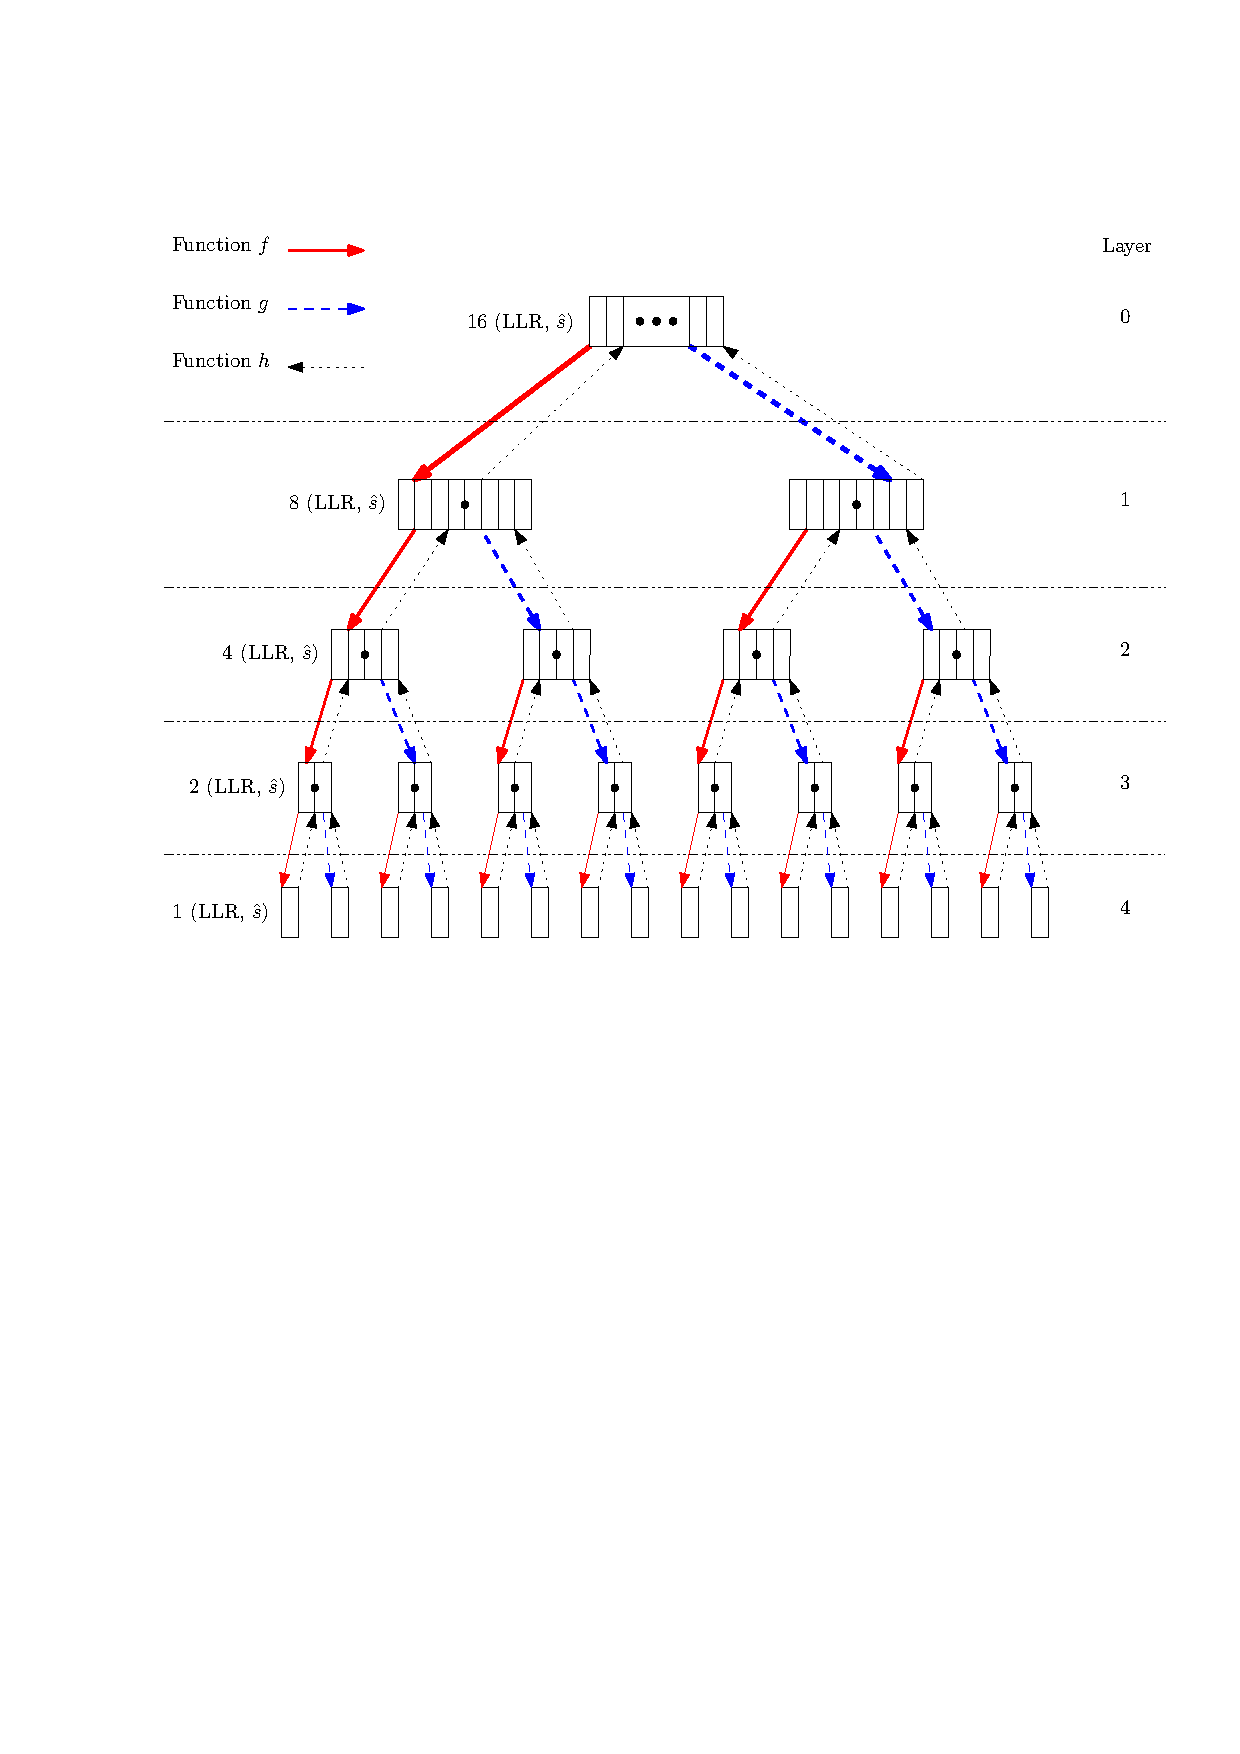
\includegraphics{polar/sc_decoder/sc_decoder}
  \caption{Full SC decoding tree ($N = 16$)}
  \label{fig:polar_sc_decoder}
\end{figure}

The Successive Cancellation (SC) decoding algorithm has been introduced by
\Arikan~\cite{Arikan2009}. It can be seen as the traversal of a binary tree
starting from the root node. For a code length $N=2^m$, the corresponding tree
thus includes $m + 1$ node layers, indexed from $d=0$ (root node layer) down to
$d=m$ (leaf nodes layers). As the tree is initially full, each layer $d$
contains $2^d$ nodes, each node of that layer $d$ containing $2^{m-d}$ LLRs
($\lambda$) and $2^{m-d}$ binary values denoted as \textit{partial sums}
($\hat{s}$). At the decoder initialization, LLRs received from the channel
($\bm{l}$) are stored in the root node. Then, the decoder performs a pre-order
traversal of the tree. When a node is visited in the downward direction, LLRs of
the node are updated. In the upward direction, partial sums are updated.
Fig.~\ref{fig:polar_sc_decoder} summarizes the computations performed in both
directions. The update functions are:
\begin{eqnarray}
\left\{\begin{array}{l c l c l}
\lambda_c &=& f(\lambda_a,\lambda_b) &=& \lambda_a \boxplus \lambda_b \approx \sign(\lambda_a.\lambda_b).\min(|\lambda_a|,|\lambda_b|)\\
\lambda_c &=& g(\lambda_a,\lambda_b,s)&=&(1-2s)\lambda_a+\lambda_b\\
(\hat{s}_{c}, \hat{s}_{d}) &=& h(\hat{s}_{a}, \hat{s}_{b}) &=& (\hat{s}_{a} \oplus \hat{s}_{b}, \hat{s}_{b}).
\end{array}\right.
\label{eq:polar_f_g_h}
\end{eqnarray}
The $f$ and $g$ functions both generate a single LLR. The $h$ function provides
a couple of partial sums. The $f$ function is the Min-Sum approximation of the
$\boxplus$ operation described in Eq.~\ref{eq:alg_ldpc_ms}. In Polar decoding
using the MS approximation does not significantly impact the decoding
performance. Thus, the MS approximation is privileged.

Before recursively calling itself on the left node, the algorithm applies the
$f$ function; respectively, before calling itself on the right node the $g$
function is applied. At the end (after the recursive call on the right node) the
$h$ function is applied. The $f$ and $g$ functions use the LLRs (read only mode)
from the current node $n_i$ in order to produce the new LLR values into
respectively left and right $n_{i+1}$ nodes. The $h$ function reads the bits
from the left and right $n_{i+1}$ nodes in order to update the bit values of the
$n_i$ node. The $\bm{\lambda}$ LLRs in the leafs are converted in the
$\bm{\hat{s}}$ bits with the hard decision function $\hat{s}_n =
\hardDec(\lambda_n)$.

Leaf nodes are of two kinds: \emph{information bit} nodes and \emph{frozen bit}
nodes. When a frozen bit leaf node is reached, its binary value is
unconditionally set to zero. Instead, when an information leaf node is reached,
its binary value is set according to the \emph{sign} of its LLR (0 if LLR is
positive, 1 otherwise). Once every node in the tree has been visited in both
directions, the decoder eventually updates partial sums in the root node and the
decoding process is terminated. If the polar code is not systematic, the decoded
bits $\bm{\hat{u}}$ are the leaf bits in the tree. Else, if the polar code is
systematic, the decoded bits $\bm{\hat{u}}$ can be directly extracted from the
root node of the polar tree in the form of a $N$-bit partial sum vectors. In the
next sections and chapters, only the systematic polar decoding is considered.

The SC algorithm is a key to construct the polar codes. A density evolution
is performed over the SC binary tree to determine the position of the frozen
bits. The idea is to construct the polar codes according to the decoder
structure. In this manuscript, the Gaussian Approximation (GA) of the density
evolution is used~\cite{Trifonov2012}.

\subsection{Successive Cancellation List Decoding Algorithm}

\begin{algorithm}
  \caption{SCL decoding algorithm.}\label{alg:polar_scl}

  % \small
  \SetKwProg{Fn}{Function}{}{}

  % \KwIn{$N$ is the frame size.}
  % \KwIn{$L$ is the number of lists (or paths) to maintain.}
  \KwData{$\lambda$ is a 2D buffer ($[L][2N]$) to store the LLRs.}
  \KwData{$\hat{s}$ is a 2D buffer ($[L][N]$) to store the bits.}

  \Fn{SCL\_decode ($N, o_{\lambda}, o_{\hat{s}}$)}
  {
    $N_{\frac{1}{2}} = N / 2$

    \uIf(\Comment*[f]{not a leaf node}){$N > 1$}
    {
      \For(\Comment*[f]{loop over the $L$ paths}){$p=0$ \textbf{to} $L-1$}
      {
        \For(\Comment*[f]{apply the $f$ function}){$i=0$ \textbf{to} $N_{\frac{1}{2}}-1$}
        {
          $\lambda[p][o_\lambda + N + i] = \bm{f}(\lambda[p][o_\lambda + i], \lambda[p][o_\lambda + N_{\frac{1}{2}} + i])$
        }
      }

      \textit{SCL\_decode ($N_{\frac{1}{2}}, o_{\lambda} + N, o_{\hat{s}}$)} \Comment*[r]{recursive call to the decoder}

      \For{$p=0$ \textbf{to} $L-1$}
      {
        \For(\Comment*[f]{apply the $g$ function}){$i=0$ \textbf{to} $N_{\frac{1}{2}}-1$}
        {
          $\lambda[p][o_\lambda + N + i] = \bm{g}(\lambda[p][o_\lambda + i], \lambda[p][o_\lambda + N_{\frac{1}{2}} + i], \hat{s}[p][o_{\hat{s}} + i])$
        }
      }

      \textit{SCL\_decode ($N_{\frac{1}{2}}, o_{\lambda} + N, o_{\hat{s}} + N_{\frac{1}{2}}$)} \Comment*[r]{recursive call to the decoder}

      \For{$p=0$ \textbf{to} $L-1$}
      {
        \For(\Comment*[f]{update the partial sums ($h$ function)}){$i=0$ \textbf{to} $N_{\frac{1}{2}}-1$}
        {
          $\hat{s}[p][o_{\hat{s}} + i] = \bm{h}(\hat{s}[p][o_{\hat{s}} + i], \hat{s}[p][o_{\hat{s}} + N_{\frac{1}{2}} + i])$
        }
      }
    }
    \Else(\Comment*[f]{a leaf node})
    {
      \textit{update\_paths ()} \Comment*[r]{update, create and delete paths}
    }
  }

  \textit{SCL\_decode ($N, 0, 0$)} \Comment*[r]{launch the decoder}

  \textit{select\_best\_path ()}
\end{algorithm}

The Successive Cancellation List (SCL) algorithm is an evolution of the
SC~\cite{Tal2011}. The SCL algorithm is summarized in
Algorithm~\ref{alg:polar_scl}. Unlike the SC algorithm, the SCL decoder builds a
list of candidate codewords along the decoding. At each call of the
\textit{update\_paths()} sub-routine (l.16), $2L$ candidates are generated. A
path metric is then evaluated to keep only the $L$~best candidates among the
$2L$ paths. The path metrics are calculated as
in~\cite{Balatsoukas-Stimming2015}. At the end of the decoding process, the
candidate codeword with the best path metric is selected in the
\textit{select\_best\_path()} sub-routine (l.18). The decoding complexity of the
SCL algorithm grows as $O(LN\log_2N)$. This linear complexity in L leads to
significant improvements in BER/FER performances compared to the SC decoder,
especially for small code lengths.

\paragraph{CRC Concatenation Scheme}

The authors in~\cite{Tal2011} observed that when a decoding error occurs, the
right codeword is often in the final list, but not with the best path metric.
They proposed to concatenate a CRC to the codeword in order to discriminate the
candidate codewords at the final stage of the SCL decoding. Indeed, this
technique drastically improves the FER performance of the decoder. This
algorithm is denoted as the \emph{CRC-Aided SCL} (CA-SCL). In terms of
computational complexity, the overhead consists in the computation of $L$ CRC at
the end of each decoding.

\subsection{Simplified Successive Cancellation Class of Algorithms}
\label{sec:alg_polar_simplified_decoders}

\begin{figure}[htp]
  \centering
  \includegraphics{polar/tree_pruning_example/tree_pruning_example}
  \caption
    [Example of polar tree pruning on a small binary tree ($N = 8$).]
    {Example of tree pruning on a small binary tree ($N = 8$). The tree is cut
    and the computations are versioned according to the location of the frozen
    bits.}
  \label{fig:tree_pruning_example}
\end{figure}

Frozen bits fully define the decoders leaf values, hence some part of the
traversal can be cut and its computation avoided, depending on the location of
the frozen bits. More generally, the tree functions can be versioned depending
on these bits. In~\cite{Alamdar-Yazdi2011}, a tree pruning technique called the
Simplified SC (SSC) was applied to SC decoding. An improved version was proposed
in~\cite{Sarkis2014a}. This technique relies on the fact that, depending on the
frozen bits location in the leaves of the tree, the definition of dedicated
nodes enables to prune the decoding tree: Rate-0 nodes (\verb|R0|) correspond to
a sub-tree whose all leaves are frozen bits, Rate-1 nodes (\verb|R1|) correspond
to a sub-tree in which all leaves are information bits, REPetition (\verb|REP|)
and Single Parity-Check (\verb|SPC|) nodes correspond to repetition and SPC
codes sub-trees. These special nodes, originally defined for SC decoding, can be
employed in the case of SCL decoding as long as some modifications are made in
the path metric calculation~\cite{Sarkis2016}. This tree-pruned version of the
algorithm is called Simplified SCL (SSCL) and the CA-SSCL when a CRC is used to
discriminate the final candidate codewords. The tree pruning technique can
drastically reduce the amount of computation in the decoding process. The
Fig.~\ref{fig:tree_pruning_example} shows that more than half of the tree nodes
can be removed for $N = 8$ (this is representative of the real-life codes).

\subsection{Adaptive Successive Cancellation List Decoding Algorithm}

The presence of the CRC can be further used to reduce the decoding time by
gradually increasing $L$. This variation of SCL is called Adaptive SCL
(A-SCL)~\cite{Li2012}. The first step of the A-SCL algorithm is to decode the
received frame with the SC algorithm. Then, the decoded polar codeword is
checked with a CRC. If the CRC is not valid, the SCL algorithm is applied with
$L=2$. If no candidate in the list satisfies the CRC, $L$ is gradually doubled
until it reaches the value $L_{max}$. In this thesis, we call this version of
the A-SCL decoding the Fully Adaptive SCL (FA-SCL) as opposed to the Partially
Adaptive SCL (PA-SCL), in which the $L$ value is not gradually doubled but
directly increased from $1$ (SC) to $L_{max}$. The simplified versions of these
algorithms are denoted PA-SSCL and FA-SSCL. In order to simplify the algorithmic
range, in the remainder of the manuscript, only the simplified versions are
considered. The use of either the FA-SSCL or the PA-SSCL algorithmic improvement
introduces no BER or FER performance degradation as long as the CRC length is
adapted to the polar code length. If the CRC length is too short, the decoding
performance may be degraded because of false detections. These adaptive versions
of SSCL can achieve higher throughputs. Indeed, a large proportion of frames can
be decoded with a single SC decoding. This is especially true when the SNR is
high. This will be further discussed in Section~\ref{sec:polar_genericity}.

\subsection{Algorithmic Comparison of the Decoders}

\begin{table}[htp]
  \centering
  \caption{Throughput and latency comparison of polar decoding algorithms.}
  \label{tab:polar_algos}
  % {\small
   \begin{tabular}{r c c c}
    \textbf{Decoding}  & \textbf{BER \& FER}   & \multirow{1}{*}{\textbf{Throughput}} & \textbf{Max. Latency}        \\
    \textbf{Algorithm} & \textbf{Performances} & ($\bm{\mathcal{T}}$)                 & ($\bm{\mathcal{L}_{worst}}$) \\
    \hline
    \hline
    SC      & poor      & medium & medium \\
    SSC     & poor      & high   & low    \\
    SCL     & good      & low    & high   \\
    SSCL    & good      & low    & medium \\
    CA-SSCL & very good & low    & medium \\
    PA-SSCL & very good & high   & medium \\
    FA-SSCL & very good & high   & high   \\
  \end{tabular}
  % }
\end{table}

In order to better distinguish all the algorithmic variations, we compare their
main features in Table~\ref{tab:polar_algos}. Each algorithm is characterized in
terms of decoding performance, throughput, and worst case latency for a software
implementation. The non-simplified versions of the adaptive SCL algorithms are
not included in the table for readability.

The SC and especially the SSC algorithms achieve very high throughput and low
latency with poor BER and FER performances. The SCL algorithm improves the
decoding performance compared to the SC algorithm, but its computational
complexity leads to an increased latency and a lower throughput. The SSCL
algorithm improves the decoding throughput and latency without any impact in
terms of BER and FER performances, as long as the tree pruning is not too deep,
as will be discussed in Section~\ref{sec:polar_genericity}. Therefore, tree
pruning is applied to all the following algorithms, namely CA-SSCL, FA-SSCL and
PA-SSCL. By applying CRC to the SCL algorithm, one can achieve better BER and
FER performances at the cost of computational complexity overhead. The Adaptive
SCL algorithms reduce the decoding time with no impact on BER and FER
performances. Furthermore, a tradeoff between throughput and worst case latency
is possible with the use of either PA-SSCL or FA-SSCL decoding algorithms.

\begin{figure}[htp]
  \centering
  \includegraphics[width=0.7\textwidth]{polar/algos_comparison/algos_comparison}
  \caption
    [Decoding performance comparison between CA-SCL and SC decoders.]
    {Decoding performance comparison between CA-SCL and SC decoders.
    Code rate $R = 1/2$, and 32-bit CRC (GZip).}
  \label{plot:polar_algos_comparison}
\end{figure}

CA-SCL decoding performances for large code lengths ($N > 2^{14}$) combined with
large list sizes ($L > 8$) are rarely presented in the literature. This is
probably due to the long simulation time required. The proposed decoders are
integrated in the \AFFECT toolbox. Therefore, multi-threaded and multi-nodes
simulations are enabled to handle such computation-demanding simulations. All
the presented simulations use the Monte Carlo method with a Binary Phase-Shift
Keying (BPSK) modulation. The communication channel is an Additive White
Gaussian Noise (AWGN) channel based on the Mersenne Twister pseudo-random number
generator (MT19937)~\cite{Matsumoto1998} and the Box-Muller
transform~\cite{Box1958}. Figure~\ref{plot:polar_algos_comparison} compares the
BER/FER performances of CA-SCL with SC decoding for a large range of code
lengths. As expected, it appears that the coding gain brought by the SCL
algorithm decreases for larger $N$ values. In the case of $N=2^{16}$, the
improvement caused by the use of the CA-SCL algorithm with $L=32$ and a 32-bit
GZip CRC (\verb|0x04C11DB7| polynomial) instead of SC is about $0.75$ dB
compared to $1.2$ dB with a polar code of size $N=2^{12}$. For larger polar
codes, $N=2^{20}$, the gain is reduced to $0.5$ dB, even with a list depth of
$128$ that is very costly in terms of computational complexity.

The tradeoffs between speed and decoding performance show some general trends.
However, the efficiency of each decoding algorithm is strongly dependent on the
polar code length, code rate, list depth and code construction. It is expected
that the best tradeoff is not always obtained with a single algorithm and
parameter set combination. It is consequently highly relevant to use a generic
and flexible decoder, that supports all variants of the decoding algorithms.
Thus, it is possible to switch from one to another as shown in the following
section.

\subsection{Generic and Flexible Decoders}
\label{sec:polar_genericity}

One of the main contribution of this thesis lies in the flexibility and the
genericity of the proposed software decoder. These terms need to be clearly
defined in order to circumvent possible ambiguity. In the remainder of the
manuscript, the \textit{genericity} of the decoder concerns all the parameters
that define the supported polar code such as the codeword length, the code rate,
the frozen bits set, the puncturing patterns and the concatenated CRC. These
parameters are imposed by the telecommunication standard or the communication
context. In the wireless communications context, these are constantly adapted by
AMC methods~\cite{Dahlman2013}. In this work, a decoder is considered
\textit{generic} if it is able to support any combination of these parameters
that can be changed during a real time execution. On the other hand, the
\textit{flexibility} of a decoder includes all the customizations that can be
applied to the decoding algorithm for a given polar code: variant of the
decoding algorithm, data quantization, list size $L$, tree pruning strategy, ...
These customizations are not enforced by a standard. The flexibility gives some
degrees of freedom to the decoder in order to find the best tradeoff between
decoding performance, throughput or latency for a given polar code.

\subsubsection{Genericity}
\label{sec:alg_polar_genericity}

In the context of wireless communications, the standards define several
different code lengths~$N$ that have to be supported to share bandwidth between
different users. This is also the case for the code rate $R$ that needs to be
adapted to the quality of the transmission channel. Therefore, a practical
implementation should be adapted to both $N$ and $R$ in real-time in order to
limit latency.

A polar code is completely defined by $N$ and the frozen bits set
$\bm{u}_{\mathcal{A}^c}$. Several methods exist to generate some "good" sets of
frozen bits~\cite{Tal2013,Trifonov2012}. The code rate $R$ depends on the size
of $\bm{u}_{\mathcal{A}^c}$. In their original form, polar code lengths are only
powers of two. The puncturing and shortening techniques
in~\cite{Wang2014,Niu2013,Miloslavskaya2015} enable to construct polar codes of
any length at the cost of slightly degraded decoding performance. The coding
scheme can be completed with the specification of a CRC.

The proposed decoders are generic regarding the code dimension $K$, the code
length $N$, the frozen bits set $\bm{u}_{\mathcal{A}^c}$ and the puncturing
patterns. All of them are dynamic parameters of the decoders and can be defined
in input files. All CRC listed in~\cite{CRCWiki2017} are available along with
the possibility to define others. It is shown in~\cite{Zhang2017} that custom
CRCs for polar codes can have a very good impact on the decoding performance.

Relying on an unique software description also implies that the tree pruning
technique has to be dynamically defined. Indeed, this technique depends on the
frozen bits set $\bm{u}_{\mathcal{A}^c}$. Not sacrificing throughput or latency
while maintaining the genericity is at the core of the proposed implementation.
Flexibility in terms of decoding algorithms, described in the following, is
necessary to deal with this challenge.

\subsubsection{Flexibility}

On the one hand, the reason for the decoder genericity is the compliance to the
telecommunication standards. On the other hand, the flexibility of the decoder
regroups several algorithmic variations that are discussed in the following.
These variations allow several tradeoffs of multiple sorts, whatever the
standard. They are all included in a single source code.

In the proposed decoders the following parameters can be changed dynamically
without re-compilation: the list size $L$, the tree pruning strategy, the
quantization of the LLRs and the different SCL variants. Each of these
adjustments can be applied to access to different tradeoffs between throughput,
latency, and error rate performance. As a consequence, one can easily fine-tune
the configuration of the software decoder for any given polar code.

\paragraph{List Size}

\begin{figure}[htp]
  \centering
  \includegraphics[width=0.70\textwidth]{polar/scl_l/scl_l}
  \caption
    [Tradeoffs between CA-SSCL decoding and throughput performances.]
    {Tradeoffs between CA-SSCL decoding and throughput performances depending on
    $L$. $N=2048$, $R=0.5$, and 32-bit CRC (GZip). For $L=1$, the SSC decoder is
    used with a ($2048$,$1024$) polar code.}
  \label{plot:polar_scl_l}
\end{figure}

As mentioned earlier, the list size $L$ impacts both speed and decoding
performance. In Figure~\ref{plot:polar_scl_l}, the throughput as well as BER and
FER performances of the CA-SSCL algorithm are shown for different $L$ values. A
($2048$,$1024$) polar code with a 32-bit CRC is considered. The computational
complexity increases linearly with $L$: the throughput is approximately halved
when $L$ is doubled, except for the case of the SC algorithm ($L=1$) which is
much faster. Indeed, there is no overhead due to the management of different
candidate paths during the decoding. For $L\geq4$ and $E_b/N_0=2$, the FER is
also approximately halved when the list size $L$ is doubled.

\paragraph{Tree Pruning Strategy}

A second degree of flexibility is the customization of the SCL tree pruning. The
authors in~\cite{Alamdar-Yazdi2011,Sarkis2016} defined dedicated nodes to prune
the decoding tree and therefore to reduce the computational complexity. In this
proposed decoder, each dedicated node can be activated separately. The ability
to activate dedicated nodes at will is useful in order to explore the
contribution of each node type on the throughput.

\paragraph{LLR Quantization}

\begin{figure}[htp]
  \centering
  \includegraphics[width=0.70\textwidth]{polar/scl_bfer/scl_bfer_rep}
  \caption
    [Impact of the \texttt{REP} node size on fixed-point SSCL decoding.]
    {Impact of the \texttt{REP} node size on fixed-point SSCL decoding.
    Code ($2048$,$1723$), $L=32$.}
  \label{plot:polar_scl_bfer_rep}
\end{figure}

Another important parameter in both software and hardware implementations is the
quantization of data in the decoder. The quantization of LLRs and partial sums
in the decoder have an impact on decoding performance. Quantized implementations
of the SC algorithm have been proposed in~\cite{Giard2016} but to the best of
our knowledge, the proposed decoder is the first SCL software implementation
that can benefit from the 8-bit and 16-bit fixed-point representations of LLRs
and internal path metrics. In the 8-bit mode LLRs and path metrics are saturated
between $-127$ and $+127$ after each operation. Moreover, to avoid overflows,
the path metrics are normalized after each \textit{update\_paths()} call (cf.
Alg.~\ref{alg:polar_scl}) by subtracting the smallest metric to each one of
them. Figure~\ref{plot:polar_scl_bfer_rep} shows the BER and FER performances of
the CA-SSCL decoder for 32-bit floating-point, 16-bit and 8-bit fixed-point
representations. One can observe that the \verb|REP| nodes degrade the decoding
performance in a 8-bit representation because of accumulation (red triangles
curve). Indeed, it is necessary to add all the LLRs of a \verb|REP| node
together in order to process it, which may lead to an overflow in the case of
fixed-point representation. It can happen when the size of the repetition nodes
is not limited ($\texttt{REP}_\texttt{2+}$). However, the size limitation of the
repetition nodes to 8 ($\texttt{REP}_\texttt{8-}$) fixes this issue.

\paragraph{Supporting Different Variants of the Decoding Algorithms}

Besides the $L$ values, the tree pruning and quantization aspects, the proposed
software polar decoder supports different variants of the SCL algorithm:
CA-SSCL, PA-SSCL, FA-SSCL.

\begin{figure}[htp]
  \centering
  \includegraphics[width=0.70\textwidth]{polar/scl_adaptive/scl_adaptive}
  \caption
    [FER and throughput of the Fully and Partially Adaptive SSCL decoders.]
    {Frame Error Rate (FER) performance and throughput of the Fully and
    Partially Adaptive SSCL decoders (FA and PA). Code ($2048$,$1723$) and
    32-bit CRC (GZip). 32-bit floating-point representation.}
  \label{plot:polar_scl_adaptive}
\end{figure}

As shown in~\cite{Sarkis2016}, the adaptive version of the SCL algorithm yields
significant speedups, specially for high SNR. The original adaptive SCL
described in~\cite{Li2012}, denoted as Fully Adaptive SCL (FA-SSCL) in this
work, gradually doubles the list depth $L$ of the SCL decoder when the CRC is
not valid for any of the generated codewords at a given stage until the value
$L_{max}$. By contrast, the adaptive decoding algorithm implemented
in~\cite{Sarkis2016}, called in this manuscript Partially Adaptive SCL
(PA-SSCL), directly increases the list depth from $1$ (SC) to $L_{max}$. In
Figure~\ref{plot:polar_scl_adaptive}, the two versions (FA-SSCL and PA-SSCL) are
compared on a ($2048$,$1723$) polar code and 32-bit CRC (GZip). The LLRs values
are based on a 32-bit floating point representation. Note that as the FER
performance of PA-SSCL and FA-SSCL are exactly the same, the related error
performance plots completely overlap. The throughput of the FA-SSCL algorithm is
higher than that of the PA-SSCL algorithm for some SNR values, depending on the
code parameters. Considering typical FER values for wireless communication
standards ($10^{-3}$ to $10^{-5}$), in the case of a ($2048$,$1723$) polar code,
the throughput of FA-SSCL is double that of PA-SSCL with $L = 8$, while it is
multiplied by a factor of $7$ with $L=32$. The drawback of FA-SSCL is that
although the average latency decreases, the worst case latency increases.

\begin{figure}[htp]
  \centering
  \includegraphics[width=0.70\textwidth]{polar/scl_bfer/scl_bfer_crc}
  \caption{Impact of the CRC size on SCL and A-SCL decoding. Code ($2048$,
    $1723$), $L=32$.}
  \label{plot:polar_scl_bfer_crc}
\end{figure}

The adaptive versions of the algorithm achieve better throughputs, but CA-SCL
may also be chosen depending on the CRC. One may observe in
Figure~\ref{plot:polar_scl_bfer_crc} that an adaptive decoder dedicated to an
8-bit CRC with a ($2048$,$1723$) polar code and $L=32$ leads to a loss of $0.5$
dB for a FER of $10^{-5}$ compared to its non adaptive counterpart.

Both polar code genericity and decoding algorithm flexibility are helpful to
support the recommendations of wireless communications in an SDR or Cloud-RAN
context. The code and decoder parameters can be dynamically changed in the
proposed decoder, while maintaining competitive throughput and latency.
However, depending on the constraints of the communication system, if the main
objective is to reach high throughputs and low latency decoding, it is possible
to trade some of the genericity and the flexibility for increased performance.
The next section discusses the polar decoder unrolling strategy.

\subsection{Unrolled Decoders}

The tree structure at the heart of SC and SCL decoders is fully determined by
the parameters of a given code instance: the code size, the code rate ($R = K /
N$), position of the frozen bits. All these parameters are statically known at
compile time. The recursive tree traversal code structure and the corresponding
tree data structure are challenging to optimize for a compiler. It is then
possible to completely flatten all the recursive calls in the tree. This leads
to a specific generated polar decoder where the $N$, $K$, $R$, the frozen bits
set, the puncturing pattern, and the CRC are fixed. This technique has been used
in previous works for both SC and SCL decoders~\cite{Sarkis2014,Cassagne2015c,
Cassagne2016b,Sarkis2016} and demonstrated higher efficiency than the generic
and flexible approach in terms of decoding throughputs and latencies. Depending
on the number of different configurations to support in a communication
standard, it is still possible to generate one specific unrolled decoder per
configuration.

\section{Turbo Codes}

\subsection{Coding Scheme}

In this sub-section, the convolutional sub-encoder is presented first and then
the turbo encoding process is detailed. The first convolutional codes have been
introduced by Peter Elias in 1955~\cite{Elias1955}. The objective was to propose
an alternative to block codes in term of codeword length flexibility:
theoretically, the length of a convolutional code is infinite. The coding scheme
output depends on the current input and on the inputs before.

\begin{figure}[htp]
  \centering
  \subfloat[][Encoding graph.]
  {
    \includegraphics[scale=1.0]{turbo/sub_encoder/sub_encoder}
    \label{fig:alg_turbo_sub_encoder_graph}
  }
  \quad
  \subfloat[][Mealy's machine.]
  {
    \includegraphics[scale=0.75]{turbo/mealy/mealy}
    \label{fig:alg_turbo_sub_encoder_mealy}
  }
  \\
  \subfloat[][Trellis representation.]
  {
    \includegraphics[scale=0.9]{turbo/trellis/trellis}
    \label{fig:alg_turbo_sub_encoder_trellis}
  }
  \caption{Example of a recursive and systematic convolutional encoder ($R =
    1/2$).}
  \label{fig:alg_turbo_sub_encoder}
\end{figure}

For a $R=1/2$ encoder, the current $p_k$ output parity bit can be expressed as a
linear combination of the $\nu$ previous bits of the message:
$p_k = \sum_{j=0}^\nu g^{(2)}_{j} u_{k-j} + \sum_{j=1}^\nu g^{(1)}_{j} p_{k-j}$,
where $\nu$ represents the number of elements memorized inside the encoder.
The sequence of elements $g_j$ is called the code-generating sequence and is
often given in octal. Fig.~\ref{fig:alg_turbo_sub_encoder_graph} presents a
convolutional encoder of rate $R = 1/2$ with a memory $\nu = 2$ ($D_0$ and $D_1$
are shift registers). Its two code-generating sequences $\bm{g^{(1)}} = (7)_8$
and $\bm{g^{(2)}} = (5)_8$ define the $c_2 = p$ output while $c_1 = u$. In
the example, the encoder has the particularity to be systematic because
$c_1 = u$ and recursive because of the feedback loop before the first shift
register $D_0$. In the literature, this type of coding scheme is called
Recursive Systematic Convolutional (RSC). Only RSC codes are considered in the
document. In Fig.~\ref{fig:alg_turbo_sub_encoder}, the number of $D$ memories
$\nu = 2$ and so, the encoder has $2^\nu = 4$ different states. Thus, a
convolutional encoder can be seen as a Mealy's machine (or a finite-state
machine) as shown in Fig.~\ref{fig:alg_turbo_sub_encoder_mealy}. The initial
state $S_0$ corresponds to $D_0 = 0$ and $D_1 = 0$, the state~$S_1$ corresponds
to $D_0 = 1$ and $D_1 = 0$, the state~$S_2$ corresponds to $D_0 = 0$ and
$D_1 = 1$ and, finally, the state~$S_3$ corresponds to $D_0 = 1$ and $D_1 = 1$.
The notation on the edges is in the form of $u/c_1c_2$. For instance, from the
state~$S_1$, if the input bit $u$ is 1, then the encoder will output two bits
$c_1 = 1$ and $c_2 = 0$ and will go in the state~$S_2$: this is denoted by
\emph{1/10} below the directed edge between $S_1$ and $S_2$.

Fig.~\ref{fig:alg_turbo_sub_encoder_trellis} introduces a new representation of
convolutional encoders: the trellis. This representation has been used the first
time by Dave Forney in 1973~\cite{Forney1973}. It is especially useful to
facilitate the understanding of the decoding process as it allows to see the
internal state of the encoder, its transitions, and the temporal evolution.
However, the purpose of this chapter is not to detail the decoding process, it
will be made in the next chapter. Considering the encoder initial state $S_0$,
from $t = 0$ the two next possible states are $S_0$ and $S_1$. At $t = 1$, the
encoder can be in state $S_0$ or $S_1$, so the next possible states are $S_0$,
$S_1$, $S_2$ or $S_3$. One can note that starting from $\nu +1$ time units, the
trellis pattern is repeated.

\begin{figure}[htp]
  \centering
  \includegraphics{turbo/encoder/encoder}
  \caption{Turbo encoder ($R = 1/3$) with two convolutional sub-encoders and a
    $\Pi$ interleaver.}
  \label{fig:alg_turbo_encoder}
\end{figure}

As mentioned before, a turbo encoder is built from two convolutional
sub-encoders. The sub-encoders can be different but it is rare.
Fig.~\ref{fig:alg_turbo_encoder} shows a generic view of the turbo encoding
process. In the example, the code rate of the turbo encoder is $R = 1/3$. This
rate is obtained from two convolutional sub-encoders of rate $R = 1/2$ (like the
one shown in Fig.~\ref{fig:alg_turbo_sub_encoder}). The two parity bits $p$ and
$p'$ are obtained from the $c_2$ outputs of the convolutional sub-encoders while
the systematic $c_1$ outputs are ignored. The first sub-encoder encodes the
$u$ input bit while the second one encode the $u'$ bit. The $u'$~bit is
determined from $u$ after the $\Pi$ interleaving process. For each $u_k$ bit
there is a single $u_k'$ associated bit in the $K$ input information bits. The
interleaving process is a key point of the decoding performance in the turbo
coding scheme, its main purpose is to fight against chunks of errors. During the
interleaving process the sequence of information bits is in the \emph{natural
order}, then these bits are permuted and the interleaver outputs a sequence of
information bits in the \emph{interleaved order}. The permutation function
defines the interleaver type. The $K$ information bits in the natural order are
given to the sub-encoder 1 while the $K$ information bits in the interleaved
order are given to the sub-encoder 2.

\subsection{Turbo Decoding Algorithm}
\label{sec:turbo_overview}

\begin{figure}[htp]
  \centering
  \includegraphics[scale=1.0]{turbo/decoder/decoder}
  \caption{Structure of a turbo decoder.}
  \label{fig:alg_turbo_decoder}
\end{figure}

The turbo decoder consists of two concatenated component decoders exchanging
soft information in terms of log-likelihood ratio (LLR) for each transmitted
information bit through an interleaver and a deinterleaver.
Fig.~\ref{fig:alg_turbo_decoder} illustrates the internal structure of a turbo
decoder. Two Soft Input Soft Output (SISO) decoders are represented with the
interleaving process $\Pi$ and the deinterleaving process $\Pi^{-1}$. In this
manuscript, we will only consider rate $R = 1/3$ codewords. $K$ represents the
number of information bits and $N$ is the codeword size: $N = K \times 3$.

\paragraph{Algorithm Outline}

Turbo decoding is carried out in multiple iterations where each iteration
consists of two component decoding phases. In each phase, a component
decoder performs a maximum a posteriori (MAP) decoding using the BCJR algorithm
\cite{Bahl1974}, which generates so-called extrinsic LLRs given the LLRs
obtained by the detector and a priori LLRs obtained from the other component
decoder. The BCJR algorithm consists of one forward and one backward traversal
on a trellis, which is defined by the underlying code. Specifically, to decode a
codeword of $K$ information bits, the BCJR algorithm performs the following
steps: (i) the branches of the trellis are weighted from the systematic LLRs
($\bm{L_s}$), the parity LLRs ($\bm{L_p}$) and the a priori information
($\bm{L_a}$); (ii) in the forward traversal step, it iteratively computes $K$
sets of forward state metrics for each transmitted information bit; (iii) in the
backward traversal step, it iteratively computes $K$ sets of backward state
metrics for each transmitted information bit; (iv) to compute the extrinsic LLRs
($L_e$), the BCJR algorithm then combines the forward and backward state
metrics. The $\bm{L_s}$, $\bm{L_p}$, $\bm{L'_p}$ vectors of LLRs correspond to
the decoder input $\bm{l}$ split in 3 sub-sets.

\begin{algorithm}
  \caption{Pseudo-code of the BCJR decoding algorithm.}
  \label{alg:alg_turbo_bcjr}

  % \small
  % \For(\Comment*[f]{Sequential loop}){$\text{all~frames}$}
  % {
    \For(\Comment*[f]{(i) parallel loop}){$k=0;~k<K;~k=k+1$}
    {
      $\boldsymbol{\gamma}^k\gets \computeGamma(L_{s}^k, L_{p}^k, L_{a}^k)$
    }

    $\boldsymbol{\alpha}^0\gets \initAlpha()$

    \For(\Comment*[f]{(ii) sequential loop}){$k=1;~k<K;~k=k+1$}
    {
      $\boldsymbol{\alpha}^k\gets \computeAlpha(\boldsymbol{\alpha}^{k-1}, \boldsymbol{\gamma}^{k-1})$
    }

    $\boldsymbol{\beta}^{K-1}\gets \initBeta()$

    \For(\Comment*[f]{(iii) sequential loop}){$k=K-2;~k \geq 0;~k=k-1$}
    {
      $\boldsymbol{\beta}^k\gets \computeBeta(\boldsymbol{\beta}^{k+1}, \boldsymbol{\gamma}^{k})$
    }

    \For(\Comment*[f]{(iv) parallel loop}){$k=0;~k<K;~k=k+1$}
    {
      $L_e^k\gets \computeExtrinsic(\boldsymbol{\alpha}^k, \boldsymbol{\beta}^{k}, \boldsymbol{\gamma}^{k}, L_{s}^k, L_{a}^k)$
    }
  % }
\end{algorithm}

Algorithm~\ref{alg:alg_turbo_bcjr} resumes the previously enumerated steps in
a pseudo-code. $\bm{\gamma}$ are the values of the trellis branches,
$\bm{\alpha}$ are the values of the nodes in the forward traversal of the
trellis and $\bm{\beta}$ are the values of the nodes in the backward traversal
of the trellis.

\begin{figure}[htp]
  \centering
  \includegraphics[width=1.0\textwidth]{turbo/encoder_lte/encoder_lte}
  \caption
    [Turbo LTE encoder and its associated 8-state trellis.]
    {Turbo LTE encoder and its associated 8-state trellis.
     $\bm{g^{(1)}} = (13)_8$, $\bm{g^{(2)}} = (15)_8$.}
  \label{fig:alg_turbo_encoder_lte}
\end{figure}

In this thesis, we focus on the turbo codes of the LTE standard~\cite{ETSI2013}
(3G and 4G mobile networks). Fig.~\ref{fig:alg_turbo_encoder_lte} gives the
definition of the LTE turbo encoder. This encoder leads to a 8-state trellis. In
the next sections and chapters, the LTE trellis is always considered.

\paragraph{Branch-metric Computations}

Let $S_j^{k+1}$ be the $j^{th}$ state associated with information bit $k+1$ and
$j \in \{0,7\}$. There are two incoming branches into state $S_j^{k+1}$. Each
incoming branch is associated with values $u^k$ and $p^k$, the $k^{th}$
information bit and the parity bit (both $\pm1$), respectively. The branch
metrics associated with states $S_i^k$ and $S_j^{k+1}$ are computed as follows:
\begin{equation}
\label{eq:turbo_gamma}
 \gamma(S_i^k, S_j^{k+1}) = 0.5(L_{s}^k + L_a^k)u^k + 0.5(L_p^k p^k).
\end{equation}
Here, $L_{s}^k$ and $L_a^k$ are the systematic channel LLR and the a priori
LLR for $k^{th}$ trellis step, respectively.
In the BCJR SISO decoder 1, the $\bm{L_{s}}$, $\bm{L_{p}}$ and $\bm{L_{a}}$
vectors of LLRs are considered (natural domain) while in the BCJR SISO decoder
2, the $\bm{L'_{s}}$, $\bm{L'_{p}}$ and $\bm{L'_{a}}$ LLRs are used instead
(interleaved domain). However, the computations in the natural and in the
interleaved domain are similar, this is why only the operations in the natural
domain are given here. Note that we do not need to evaluate the branch metric
$\gamma(s^k , s^{k+1})$ for all 16 possible branches, as there are only four
different branch metrics:
$\gamma^k_0 = 0.5(L_{s}^k + L_a^k + L_p^k)$,
$\gamma^k_1 = 0.5(L_{s}^k + L_a^k - L_p^k)$, $-\gamma^k_0$, and $-\gamma^k_1$.

\paragraph{Forward and Backward State-metric Computations}

The forward state metrics can be computed iteratively from trellis step to
trellis step. The forward state metrics of step $k+1$ correspond to the vector
$\bm{\alpha^{k+1}} = [\alpha_0^{k+1}, ... ,\alpha_7^{k+1}]$, where the
$j^{th}$ forward state metric $\alpha_j^{k+1}$ only depends on two forward
state metrics of stage $k$. These state metrics are computed by:
\begin{equation}
  \label{eq:turbo_alpha}
  \alpha_j^{k+1} =
  \maxstar_{i \epsilon F} ( \alpha_i^k + \gamma(S_i^k, S_j^{k+1}) ),
\end{equation}
where the set $F$ contains the two indexes of the states in step $k$ connected
to state $S_j^{k+1}$ (as defined by the trellis). The $\maxstar$ operator is
defined as:
\begin{equation}
   \maxstar(a,b) = \max(a,b) + \log(1 + \exp(-|a-b|)),
\end{equation}
where $\log(1 + \exp(-|a-b|))$ is a correction term.
Computation of the backward state metrics is similar to that of the forward
trellis traversal in Eq.~\ref{eq:turbo_alpha}. The vector of backward state
metrics, denoted by $\bm{\beta^k} = [\beta_0^k, ..., \beta_7^k]$, is
computed as:
\begin{equation}
  \label{eq:turbo_beta}
  \beta_j^k =
  \maxstar_{i \epsilon B} ( \beta_i^{k+1} + \gamma(S_j^k, S_i^{k+1}) ),
\end{equation}
where $B$ is the set containing the indexes of states in step $k+1$ connected to
state $S_j^k$ as defined by the trellis.

\paragraph{Extrinsic LLR Computations}

After the forward and backward iterations have been carried out, the extrinsic
LLRs for the $k^\text{th}$ bit are computed as:
\begin{equation}
  \label{eq:turbo_ext}
  \begin{aligned}
  L_e^k = \maxstar_{\{S_k, S_{k+1}\}\epsilon U^1}\big( \alpha_i^k + \beta_j^{k+1} +
  \gamma(S_i^k, S_j^{k+1}) \big) \\
  - \maxstar_{\{S_k, S_{k+1}\}\epsilon U^{-1}}\big( \alpha_i^k + \beta_j^{k+1} +
  \gamma(S_i^k, S_j^{k+1}) \big) \\
  - L_{s}^k - L_a^k,
  \end{aligned}
\end{equation}
where the sets $U^1$ and $U^{-1}$ designate the set of states connected by paths
where $u^k=1$ and the set of states connected by paths where $u^k=-1$,
respectively (because of the BPSK modulation).

\begin{figure}[htp]
  \centering
  \includegraphics[width=0.7\textwidth]{turbo/iterations/iterations}
  \caption
    [Decoding performance of the turbo decoder depending on the number of
     iterations.]
    {Decoding performance of the turbo decoder depending on the number of
     iterations. LTE code, $K = 6144$, $R = 1/3$, MAP algorithm.}
  \label{plot:alg_turbo_iterations}
\end{figure}

Fig.~\ref{plot:alg_turbo_iterations} shows the decoding performance of the turbo
decoder depending on the number of iterations. The biggest code from the
LTE standard is evaluated ($K = 6144$ and $R=1/3$). It has been shown that the
BCJR is in fact an instance of the BP algorithm~\cite{McEliece1998}. In one
iteration, the BCJR decoder 1 and 2 are run. Thus, the computational complexity
of one turbo decoding iteration is higher than one LDPC BP decoding iteration.

\paragraph{Approximation of the MAP Operations in the BCJR Decoder}

\begin{figure}[htp]
  \centering
  \includegraphics[width=0.7\textwidth]{turbo/approximations/approximations}
  \caption
    [Decoding performance of the turbo decoder depending on the approximations.]
    {Decoding performance of the turbo decoder depending on the BCJR algorithm
     approximations. The maximum a posteriori (MAP), the max-log-MAP (ML-MAP)
     and the enhanced max-log-MAP (EML-MAP, $\alpha = 0.75$) are evaluated.
     $K = 6144$, $R=1/3$ and 6 decoding iterations.}
  \label{plot:alg_turbo_approximations}
\end{figure}

The $\maxstar$ operator of the MAP algorithm is compute intensive, mainly due to
the logarithm and exponential functions in the correction term. It can be
approximated as follow: $\maxstar(a,b) \approx \max(a,b)$. The correction term
is simply removed. This approximation is called the \emph{max-log-MAP} algorithm
(ML-MAP). Its low computational complexity makes efficient software and hardware
implementations possible. However, the ML-MAP algorithm negatively affects the
decoding performance. It this then possible to partially recover the error-rate
performance loss by scaling the extrinsic LLRs in the turbo decoder by a factor
$\alpha$: this is called the \emph{Enhanced} max-log-MAP (EML-MAP)
algorithm~\cite{Vogt2000,Studer2011}. The impact of the approximations on the
decoding performance is shown in Fig.~\ref{plot:alg_turbo_approximations}.

\paragraph{Impact of the Quantification on the Error-rate}

\begin{figure}[htp]
  \centering
  \includegraphics[width=0.7\textwidth]{turbo/quantification/quantification}
  \caption
    [BER and FER of the turbo decoder for $K = 6144$ (6 iters) and $R=1/3$.]
    {Bit Error Rate (BER) and Frame Error Rate (FER) of the decoder for $K =
    6144$, $R=1/3$ and 6 decoding iterations. Enhanced max-log-MAP algorithm
    ($\alpha = 0.75$).}
  \label{plot:alg_turbo_quantification}
\end{figure}

Fig.~\ref{plot:alg_turbo_quantification} shows the decoding performance of the
turbo decoder depending on the quantification. \emph{float} is the ideal
decoding performance of the EML-MAP algorithm on 32-bit floating-point.
\emph{int-16} is a quantified version of the decoder, on 16-bit and with
fixed-point arithmetic computations. Before to enter in the decoder, the
$\bm{l}$~LLRs are converted from a floating-point representation to a
fixed-point representation: they are saturated on $s = 6$ bits, of which $d = 3$
bits are dedicated to the decimal part ($Q_{s,d}$). Inside the decoder, the
saturation is made over 16 bits ($s = 16$). One can note that there is no
decoding performance degradation. Finally, \emph{int-8} is the 8-bit quantified
version of the decoder. Compared to the 16-bit version, the decimal part of the
8-bit version is represented with 2 bits ($Q_{6,2}$) instead of 3. The internal
saturations are on 8-bit. This version shows a 0.1 dB degradation. The limited
dynamic of 8-bit format together with early saturation inside the decoder are
responsible for this small performance loss.

\section{Sparse Code Multiple Access}

\subsection{Presentation and Related Works}

Non-Orthogonal Multiple Access (NOMA) mechanisms are investigated as means to
improve the fifth-generation mobile communication systems (5G)~\cite{Islam2017}
to realize massive connectivity and to reduce bit error rates. Sparse Code
Multiple Access (SCMA) is a NOMA mechanism that offers better bit error rate
performance and higher spectral efficiency, while the sparsity of the codebooks
ensures lower complexity of decoding compared to other non-orthogonal
modulations~\cite{Nikopour2013}. SCMA is a promising candidate for 5G
communication systems since it provides up to 3 times more connectivity by
spreading the information of each user's codebook over sets of shared OFDM
frequency tones~\cite{Altera2015}. According to the NGMN white
paper~\cite{Alliance2015}, 5G targets more diverse scenarios compared to 4G.
Applications can be broadband support in dense areas, low latency connectivity
for Augmented Reality (AR) and reliable communication for intelligent industrial
controls, Internet of Things (IoT) or Internet of Mission Critical Things
(IoMCT). Unfortunately, the massive connectivity and spectral efficiency of SCMA
come at the cost of high complexity in the decoder, making the design of high
throughput and low complexity decoders a challenge~\cite{Lu2015}.

Exploiting sparsity of the codebooks, Belief Propagation (BP) or Message Passing
Algorithm (MPA) decoders were introduced to achieve near Maximum Likelihood
performance with lower complexity~\cite{Zhang2014a}. Substantial research works
were conducted on improving SCMA decoders to satisfy the uplink requirements of
5G. Indeed, MPA is populated with many exponential computations to compute the
extrinsic information and probabilities of the received signal. This is based on
modeling the channel noise with a Gaussian probability density function (PDF). A
classical improvement to this bottleneck is the computation of extrinsic
information in the logarithm domain, which led to develop the log-MPA decoder.
In~\cite{Liu2016}, fixed-point and floating-point implementations of the MPA and
log-MPA on FPGA are studied. The bit error rate performance and complexity of
the MPA and log-MPA are compared and it is concluded that using log-MPA with 4
message passing iterations achieves a good tradeoff between performance and
complexity. In~\cite{Bayesteh2015}, several complexity reduction techniques are
proposed to increase the system throughput. These techniques are 1) SCMA
codebook design with minimum number of projections, 2) clustered MPA (CMPA)
which defines sub-graphs in MPA and runs MPA on them, and 3) selected
exponential computations. In~\cite{Du2016} an adaptive Gaussian approximation
is used to unselect the edges of the graph with smaller modulus. In addition,
mean and variance feedbacks are employed to compensate information loss caused
by unselected edges. User's codebooks play an important role for fast
convergence of the MPA or log-MPA. As investigated in~\cite{Taherzadeh2014,
Peng2017,Yan2017}, revisiting codebook design can help to reduce the number of
iterations needed for MPA decoding of SCMA. In~\cite{Jia2018}, an improved MPA
is proposed which eliminates determined user codewords after a certain number of
iterations and continue the iterations for undetermined user's codewords.
Similarly, in~\cite{Yang2016}, a belief threshold is set to choose the most
reliable edge probabilities and continue the iterations for the others. A
Shuffled MPA (S-MPA) is introduced in~\cite{Du2016a}. S-MPA is based on
shuffling the messages between function nodes and variable nodes. As a result,
the convergence rate is accelerated. A Monte Carlo Markov Chain Method is
proposed in~\cite{Chen2016} to decode SCMA signals and sphere decoding is also
explored in~\cite{Yang2017,Wei2017} for SCMA receiver design.

The main difference between this work and previously cited works is to combine
an analytic view of MPA complexity with hardware and resource aware programming,
and to exploit hardware features available in general purpose processors (GPPs).
The SCMA decoding algorithms are revised in light of the needs of Cloud Radio
Access Networks (Cloud-RANs).

% The main difference between this work and previously cited works is that the
% present manuscript combines an analytic view of MPA complexity with hardware and
% resource aware programming, exploiting hardware features available in general
% purpose processors (GPPs). The SCMA decoding algorithms are revised in light of
% the needs of Cloud Radio Access Networks (Cloud-RANs) and to take full advantage
% of key hardware features available in GPPs such as their SIMD engine. In the
% early 2000s, the performance of many processors improved significantly due to
% clock rate increases. This increase of performance needed very minimal if any
% programming effort, however the drawbacks of high clock rate was more power and
% energy consumption, overheating of processors, leakage currents and signal
% integrity problems. These disadvantages led designers to follow new paradigms
% such as thread-level and data-level parallelisms that provide good performance
% at lower clock speeds. Another challenge was data access efficiency in cache and
% RAM for performance critical algorithms. Higher performance also came from
% improved cache access efficiency of heterogeneous processors and parallel access
% to the L1 cache through vectorized instructions. Therefore, complicated and
% control heavy algorithms such as MPA have to be adapted for efficient execution
% on heterogeneous architectures and their exploitable parallelism must be
% expressed at every level of the code, whether in arithmetic or memory access
% instructions. Particularly, various Single Instruction Multiple Data (SIMD)
% extensions and thread-level parallelism are used to increase the throughput of
% MPA decoding on various platforms.

% This work reports on two contributions that can be useful for any variation of
% the aforementioned MPA. First, MPA and log-MPA have been adapted to use SIMD
% extensions leveraging the available data-level parallelism. The algorithms are
% revised to have aligned and contiguous access to memory, which is crucial to
% achieve high memory throughput. Various SIMD instruction set architectures
% (ISAs) such as Advanced Vector Extensions (AVX), Streaming SIMD Extension (SSE),
% Knights Corner Instruction (KNCI) and ARM\R NEON are used to enhance the
% performance of various parts of the algorithm. Multi-threaded programming
% technique and power efficiency are also studied in this paper.

% Second, efforts have been made to reduce the high dynamic ranges and high
% storage burden that are induced by the numerous calculations of the exponential
% function embedded in MPA, which is one of its main points of congestion. To
% eliminate calculations of the exponentials in the MPA, this paper uses
% approximate modeling of noise. Indeed, a Gaussian Probability Density Function
% (PDF) is estimated with sub-optimal, bell shaped, polynomial PDFs. Using
% polynomial PDFs enables a significant throughput improvement with a very small
% degradation on the bit error rate performance. In addition, this technique
% enables to use vectorized instructions for the calculation of the probabilities,
% as opposed to log-MPA. Details will be explained in the sequel. The impacts of
% turbo codes~\cite{Berrou1993}, polar codes~\cite{Arikan2009} and LDPC
% codes~\cite{Gallager1962,MacKay1995} are investigated.

The next sub-sections present the SCMA from a digital communication system
point of view and, then, the Maximum Likelihood, MPA and log-MPA decoding
methods are presented. Finally, our Estimated-MPA (E-MPA) algorithm is
described.
% The paper is organized as follows, Section~\ref{sec:scma_detection} introduces
% the SCMA algorithm. Maximum Likelihood, MPA and log-MPA decoding methods are
% explained in this section as a background to this research.
% Section~\ref{sec:opt_scma} elaborates on proposed improvements such as
% vectorizing the algorithm, exponential estimations, contiguous access to memory
% and other hardware oriented techniques. Section~\ref{sec:scma_perf} explores the
% bit error rate performance as well as the throughput, the latency, the power
% consumption, and the energy efficiency of the proposed MPA and log-MPA
% implementations. Some profiling metrics are given to better understand the
% results. Section~\ref{sec:scma_fec} is dedicated to study the effects of
% suggested techniques on block error rate after channel coding. Finally, the main
% findings of this research are summarized in Section~\ref{sec:scma_conclusion}.

\subsection{Overview of the SCMA System Model}
\label{sec:scma_overview}

In this section, symbols $\mathbb{B}$, $\mathbb{N}$, $\mathbb{Z}$, $\mathbb{R}$
and $\mathbb{C}$ denote binary, natural, integer, real and complex numbers.
Scalar, vector and matrix are presented as $x$, $\bm{x}$, $\bm{X}$ respectively.
The $n^\text{th}$ element of a vector denoted by $\bm{x}_n$ and $\bm{X}_{n,m}$
is the element of $n^\text{th}$ row and $m^\text{th}$ column of matrix $\bm{X}$.
Notation $\diag(x)$ shows a diagonal matrix where its n'th diagonal element is
$\bm{x_n}$. In addition, the transpose of a matrix is expressed as $\bm{X^T}$.

An SCMA encoder with $J$ users (layers) and $K$ physical resources is a function
that maps a binary stream of data to $K$-dimensional complex constellations
$f : \mathbb{B}^{log_{2}(M)} \rightarrow \mathbb{X}, x = f(\bm{b})$ where
$\bm{X} \subset \mathbb{C}^k$. The $K$-dimensional complex codeword $x$ is a
sparse vector with $N < K$ non-zero entries. Each layer $j=1, ..., J$ has its
own codebook to generate the desired codeword according to the binary input
stream. Fig.~\ref{fig:scma} shows the SCMA uplink chain with $J = 6$, $K = 4$
and $N = 2$. SCMA codewords are spread over $K$ physical resources, such as OFDM
tones. Fig.~\ref{fig:scma_enc} shows that in the multiplexed scheme of SCMA, all
chosen codewords of the $J$ layers are added together after being multiplied by
the channel coefficient $\bm{h}_j$. Then, the entire uplink chain is shown in
Fig.~\ref{fig:scma_codec}. The output of the SCMA encoder is affected by the
white additive noise $\bm{n}$:
\begin{equation}
  \label{eq:scma_1}
  \bm{y} = \sum\limits_{j=1}^J \diag(\bm{h}_j)\bm{x}_j+\bm{n},
\end{equation}
where $\bm{x}_j=(x_1,...,x_{Kj})^T$ and $\bm{h}_j=(h_1,...,h_{Kj})^T$ are
respectively codeword and channel coefficients of layer $j$.
Considering the digital communication chain presented in
Fig.~\ref{fig:ctx_com_chain} the SCMA encoder can be seen as a digital modulator
and the SCMA decoder can be seen as a digital demodulator.

\subsection{SCMA Decoding Schemes}
\label{sec:scma_detection}

\paragraph{Maximum Likelihood}
\label{sec:scma_ml}

For an arbitrary codeword, the optimum decision, i.e. the one that minimizes the
likelihood of transmission errors after decoding, is the one resulting from the
Maximum Likelihood (ML) estimation, which can be described as:
\begin{equation}
  \label{eq:scma_2}
  \bm{\hat{x}} = \argmin_{c \in \bm{X}}||\bm{y - c}||^2,
\end{equation}
given the received codeword. In \eqref{eq:scma_2}, the soft outputs
$\hat{\bm{x}}$ are LLRs (denoted as $\bm{l}$ in Fig.~\ref{fig:ctx_com_chain}).
When a signal is transmitted over an AWGN channel (of $\sigma^2$ variance), the
probability function $\prob(\bm{y}|\bm{c})$ can be expressed as:
\begin{equation}
  \label{eq:scma_4}
  \prob(\bm{y}|\bm{c}) = \frac{1}{\sqrt{2\pi}\sigma}\exp
  \Bigg(-\frac{||\bm{y}-\bm{c}||^2}{2\sigma^2}\Bigg).
\end{equation}

\begin{figure}[htp]
  \centering
  \subfloat[][SCMA encoder with 6 users (layers) and 4 physical resources.]{
    \label{fig:scma_enc}
    \includegraphics{scma/codec/codec_enc}
  }
  \\
  \subfloat[][SCMA uplink chain with channel coding.]{
    \label{fig:scma_codec}
    \includegraphics{scma/codec/codec_chain}
  }
  \\
  \subfloat[][Factor graph representation of a decoder.]{
    \label{fig:scma_dec_graph}
    \includegraphics{scma/codec/codec_graph}
  }
  \quad
  \subfloat[][Message Passing Algorithm based on Bayesian factor graph:\linebreak
              (I)   Resource to user message,
              (II)  Guess swap at each user and user to resource message,
              (III) Final guess at each user.]{
    \label{fig:scma_dec_alg}
    \includegraphics{scma/codec/codec_dec}
  }
  \caption
    [SCMA system model, encoding and decoding schemes.]
    {SCMA system model, encoding and decoding schemes.}
  \label{fig:scma}
\end{figure}

Although the ML method provides the best guess for $\bm{\hat{x}}$, performing
the computation with this method requires unacceptable complexity in real
applications. In the case of six users and codebooks matrix size $4\times4$ as
in Fig.~\ref{fig:scma_enc}, the calculation of the soft output for each bit
in \eqref{eq:scma_4} needs 4096 exponential function computations, which is
unacceptable. Nevertheless, the result of this method is used to compare with
practical methods to characterize the BER performance degradation of MPA and
log-MPA.

\paragraph{Message Passing Algorithm}
\label{sec:scma_mpa}

Fig.~\ref{fig:scma_dec_graph} shows a Bayesian factor graph representation of an
MPA decoder with six users and four physical resources. Thanks to the sparsity
of the codebooks, exactly three users collide in each physical resource. There
are four possible codewords for each of the three connected user's codebooks
which gives 64 possible combined codewords in each physical resource. In the
first step of the MPA, the 64~distances between each possible combined codeword
and the actual received codeword are calculated:
\begin{equation}
  \label{eq:scma_5}
  d_{RES  \beta}(\bm{m}, \bm{H}) =
  \underset{l \subset \zeta, m_u\in\{1,...,K\}}{||\bm{y}_\beta -
  \sum \bm{h}_{l,m_u} \bm{x}_{l,m_u} ||},
\end{equation}
$\zeta$ is the set of users connected to resource $\beta$ and the
considered codeword is denoted as $m$. For instance, \eqref{eq:scma_5} can be
rewritten for resource 4 as:
\begin{equation}
  \label{eq:scma_6}
  \begin{split}
  d_{RES 4}(m_2,m_4,m_6,\bm{h}_2, \bm{h}_4, \bm{h}_5) =
  \underset{m_{2,4,6}=1,2,3,4}{|| \bm{y_4} - \Big(\bm{h}_2\bm{x}_2(m_2) +
  (\bm{h}_4\bm{x}_4(m_4) + (\bm{h}_5\bm{x}_5(m_5) \Big) ||}.
  \end{split}
\end{equation}
In which $m_2$, $m_4$, $m_5$ indicate the different codewords for users 5, 4,
and 2 in \eqref{eq:scma_6}. Assuming perfect channel estimation and Gaussian
noise, these Euclidean distances can be expressed as probabilities using
\eqref{eq:scma_7}:
\begin{equation}
  \label{eq:scma_7}
  \Psi(d_{RES \beta}) = \exp \Bigg(-\frac{d_{RES \beta}^2}{2\sigma^2} \Bigg).
\end{equation}
After calculating the residual probability of each codeword with
\eqref{eq:scma_7}, iterative MPA starts exchanging beliefs (probabilities) on
possible received codewords among the users and resources nodes of the
factor-graph. According to Fig.~\ref{fig:scma_dec_alg} (I), a message from
resources to users has been defined to contain extrinsic information of two
other connected users. For instance, a message from resource 4 to user 2
containing the probability information of codeword $i$ can be expressed as:
\begin{equation}
  \label{eq:scma_8}
  \begin{split}
  \mu_{RES4 \rightarrow UE2}(i) = \sum\limits_{j=1}^4 \sum\limits_{i=1}^4 \Psi
  \Big(d_{RES4}(i,j,k,\bm{H}) \Big)
  \times \mu_{UE4 \rightarrow RES4}(j) \times \mu_{UE5 \rightarrow RES4}(k).
  \end{split}
\end{equation}
As shown in Fig.~\ref{fig:scma_dec_alg}(II) there are only two resources
connected to each user. A message from a user to a resource is a normalized
guess swap at the user node:
\begin{equation}
  \label{eq:scma_9}
  \mu_{UE3 \rightarrow RES1}(i) = \frac{\mu_{RES3 \rightarrow UE3}(i)}
  {\sum_i\mu_{RES3 \rightarrow UE3}(i)},
\end{equation}
message passing between users and resources (see \eqref{eq:scma_8} and
\eqref{eq:scma_9}) will be repeated three to eight times to reach the desired
decoding performance. The final belief at each user $B(i)$ is the multiplication
of all incoming messages as illustrated in Fig.~{\ref{fig:scma_dec_alg}}(III)
and \eqref{eq:scma_10} for UE3 and codeword $i$. Finally, \eqref{eq:scma_11} is
used to calculate soft outputs for bit $b_x$:
\begin{equation}
  \label{eq:scma_10}
  B_3(i) = \mu_{RES1 \rightarrow UE3}(i) \times \mu_{RES3 \rightarrow UE3}(i),
\end{equation}
\begin{equation}
  \label{eq:scma_11}
  \bm{\hat{x}} = \ln \Bigg( \frac{\prob(\bm{y}|b_x=0)}{\prob(\bm{y}|b_x=1)} \Bigg) =
  \ln \Bigg( \frac{\sum_m B_m(i)_{~\text{when}~b_x=0}}{\sum_m B_m(i)_{~\text{when}~b_x=1}}
  \Bigg).
\end{equation}

\paragraph{Log-MAP}
\label{sec:scma_log-map}

Since calculation of exponentials in \eqref{eq:scma_7} requires relatively high
computational effort, changing the algorithm to logarithmic domain using the
Jacobi formula \eqref{eq:scma_12} is a classical improvement of MPA:
\begin{equation}
  \label{eq:scma_12}
  \ln \Bigg( \sum\limits_{i-1}^N\exp(f_i) \Bigg) \approx \max\{f_1,f_2,...,f_N\}
\end{equation}
using Jacobi formula, \eqref{eq:scma_8} can be reduced to:
\begin{equation}
  \label{eq:scma_13}
  \mu_{RES1 \rightarrow UE5}(i) = \underset{j,k=1,...,4}
  {\max \Bigg(-\frac{d_{RES1}^2(i,j,k,\bm{H})}{2\sigma^2} \Bigg)} +
  \mu_{UE2 \rightarrow RES1}(j) + \mu_{UE3 \rightarrow RES1}(k),
\end{equation}
due to elimination of exponential's high dynamic ranges, there is no need to
normalize the guess swap and \eqref{eq:scma_9} will be:
\begin{equation}
  \label{eq:scma_14}
  \mu_{UE3 \rightarrow RES1}(i) = \mu_{RES3 \rightarrow UE3}(i).
\end{equation}
The rest of the algorithm can be expressed as follows:
\begin{equation}
  \label{eq:scma_15}
  B_3(i) = \mu_{RES3 \rightarrow UE3}(i) + \mu_{RES1 \rightarrow UE3}(i),
\end{equation}
\begin{equation}
  \label{eq:scma_16}
  \bm{\hat{x}} = \max_i(B_m(i))_{~\text{when}~b_x=0} - \max_i(B_m(i))_{~\text{when}~b_x=1}.
\end{equation}

\paragraph{Estimated-MPA (E-MPA)}

Computation of the exponentials in \eqref{eq:scma_7} is one of the most
important bottlenecks of the MPA algorithm. It is possible to further accelerate
the computation by using proper estimations. The exact exponential computation
is not essential to produce a satisfying estimation in the MPA algorithms.
Considering that \eqref{eq:scma_7} represents a Gaussian PDF, it can be replaced
by sub-optimal bell-shaped polynomial distributions to model the noise. It will
be shown in Section~\ref{sec:eval_scma_throughput} that using a
polynomial estimation can increase the throughput while leading to marginal bit
error rate degradation after the MPA decoding. However, these estimated
probabilities cause small degradations of the FER performance after the channel
decoding (cf. Section~\ref{sec:scma_fec}). The proposed PDF must satisfy two
conditions to be valid: 1) it must be positive and lower bounded at zero, 2) its
integral over $(-\infty, \infty)$ must be equal to 1. The following function is
suggested to estimate the exponentials:
\begin{equation}
  \label{eq:scma_18}
  \Psi^{'}_{d_{RES \beta}} = \frac{2 / \pi}{2\sigma^2 + 4d^4_{RES \beta}}.
\end{equation}
The computation of $\Psi^{'}$ is faster than the original
$\Psi$~\cite{Ghaffari2017}. The probabilities produced using \eqref{eq:scma_7}
and \eqref{eq:scma_18} are normalized according to \eqref{eq:scma_9}.
Furthermore, the numerator $2/\pi$ does not play an important role in MPA and
can be uniformly eliminated from all calculations to reduce the computational
effort. Thus,
\begin{equation}
  \label{eq:scma_19}
  \Psi^{'}_{d_{RES \beta}} \approx \frac{1}{2\sigma^2 + 4d^4_{RES \beta}},
\end{equation}
can be used as a systematic replacement to the exponential calculations.

\subsubsection{Uncoded Error Performance}
\label{sec:scma_perf}

\begin{figure}[htp]
  \centering
  \includegraphics[width=0.7\linewidth]{scma/ber_uncoded/ber_uncoded}
  \caption{BER performance comparison of ML, MPA and E-MPA for 5 iterations.}
  \label{plot:scma_ber_uncoded_a}
\end{figure}

\begin{figure}[htp]
  \centering
  \includegraphics[width=0.7\linewidth]{scma/ber_uncoded_iter/ber_uncoded_iter}
  \caption{Convergence behavior of E-MPA and MPA decoding algorithm.}
  \label{plot:scma_ber_uncoded_b}
\end{figure}

Fig.~\ref{plot:scma_ber_uncoded_a} compares the ML, MPA and E-MPA SCMA decoding
algorithms. There are very small differences in the bit error rate performance
of the three decoders (less than 0.10 dB). Although both MPA and E-MPA show
their optimum behavior with 5 iterations, the convergence behavior of the two
methods are different as illustrated in Fig.~\ref{plot:scma_ber_uncoded_b}.
E-MPA has a slower convergence rate for less than three iterations. This
phenomenon is expected as the probability functions produced by bell-shaped
polynomial PDF do not have the quality of probabilities produced by
exponentials. However, the convergence behavior is almost identical for more
than 4 iterations.

\subsubsection{Coded Error Performance}
\label{sec:scma_fec}

In the previous sections, algorithmic approximations have been proposed through
the E-MPA SCMA decoding algorithms. These approximations lead to drastic
reductions of the processing time and to an increase of the processing power
efficiency (it will be discussed later in Section~x and Section~y). This is done
with little degradation of the BER performance in an uncoded environment.
Nevertheless, in a full communication chain, multiple access algorithms are
closely linked to the forward error correction modules. Indeed, the output of
the channel encoder is the input of the SCMA encoder/modulator and the output of
the SCMA decoder/demodulator is the input of the channel decoder. In this
section, we propose to evaluate the decoding performance of the SCMA associated
to different channel codes. Exceptionally in the manuscript, the SCMA
encoder/decoder take the place of the BPSK modulator/demodulator used everywhere
else.

For the error rate evaluation, the turbo decoders have been retained since they
are used in the LTE standard~\cite{ETSI2013} (3G/4G mobile networks) as well
as the polar and LDPC codes present in many wireless standards like the
5G~\cite{ETSI2018} and the Wi-Fi.

\begin{figure}[htp]
  \centering
  \subfloat[][Code rate $R=1/3$.]
  {
    \includegraphics[width=0.70\textwidth]{scma/fec/fec_1_3}
    \label{plot:scma_fec_a}
  }
  \\
  \subfloat[][Code rate $R=1/2$.]
  {
    \includegraphics[width=0.70\textwidth]{scma/fec/fec_1_2}
    \label{plot:scma_fec_b}
  }
  \caption
    [FER evaluation of MPA and E-MPA decoders combined with channel coding.]
    {FER evaluation of SCMA MPA and E-MPA decoders combined with LDPC, polar
    and turbo codes.}
  \label{plot:scma_fec}
\end{figure}

Fig.~\ref{plot:scma_fec} shows the FER performances of MPA and E-MPA decoders
when combined with different channel codes. For a matter of reproducibility, the
full parameters of the FEC used are reported below. This evaluation does not
claim  any novelty in channel coding, however, we found crucial to validate our
proposed SCMA optimizations in a sufficiently complete communication chain.

\paragraph{Turbo codes}

In a first validation, the turbo code from the LTE standard is used. In the
decoder, 6 iterations are done. The two sub-decoders implement the Enhanced
Max-Log Maximum A-Posteriori algorithm (EML-MAP)~\cite{Robertson1995} with a
$\alpha = 0.75$ scaling factor~\cite{Vogt2000}. In Fig.~\ref{plot:scma_fec_a},
the rate is $R \approx 1/3$, no puncturing is performed, the number of
information bits $K$ is 1024 and the codeword length $N$ is 3084. In
Fig.~\ref{plot:scma_fec_b}, $R \approx 1/2$ with the puncturing of half of the
parity bits, $K=2048$, and $N=4108$.

\paragraph{LDPC codes}

In a second set of validations, the LDPC codes used in this paper are based on
MacKay's matrices that have been taken from its personal
webpage\footnote{MacKay's webpage: \url{http://www.inference.org.uk/mackay/codes/data.html}}.
In Fig.~\ref{plot:scma_fec_a}, the matrix used is ($K=272$, $N=816$), and in
Fig.~\ref{plot:scma_fec_b} the matrix is ($K=2000$, $N=4000$). In both figures,
the decoder used is a Belief Propagation (BP) decoder with an Horizontal Layered
scheduling~\cite{Yeo2001}. For the update rules, the Sum-Product Algorithm (SPA)
has been used~\cite{MacKay1999}. The number of iterations is 100.

\paragraph{Polar codes}

In the final validation, polar codes are built by suitably selecting the frozen
bits. We used the Gaussian Approximation (GA) technique of~\cite{Trifonov2012}.
The input SNR for the code construction with the GA is 1 dB, which apparently is
very low considering that the SNR are 4 to 5 dB in the convergence zone. This is
motivated by the fact that the GA algorithm is designed to work with the BPSK
modulation. Using SCMA completely modifies the histogram of the LLR values for a
given SNR. Therefore, a shift on the input SNR of the GA algorithm must be
applied in order to efficiently select the frozen bits. If this shift is
not applied, the decoding performances of the polar code degrades drastically.
The number of information bits and the codeword length are ($K=682$, $N=2048$)
in Fig.~\ref{plot:scma_fec_a} and ($K=2048$, $N=4096$) in
Fig.~\ref{plot:scma_fec_b}. The decoder is the CRC-Aided Successive Cancellation
List (CA-SCL) decoder with $L=32$ (the 32-bit GZIP CRC is used).

\paragraph{Effects of E-MPA on Error Correction}
\label{sec:scma_fec_e-mpa}

In Fig.~\ref{plot:scma_fec}, the number of iterations of the SCMA demodulator is
5. The objective of simulating multiple channel codes is not to compare them
with each other. A fair comparison of the different channel codes would indeed
impose using the same code lengths and more importantly their computational
complexity should be compared, which is not the case here. Our goal here is to
study the impact of using E-MPA on the BER and FER performances when the channel
codes are included in the communication chain. For each channel code, two curves
are plotted: one for the E-MPA and the other for the MPA. Only 0.2 to 0.4 dB
separate the two versions of the algorithm for all the considered channel codes.
These results show the extent to which uncertainty of estimations affects
channel coding. The decoding speed improvement brought by the E-MPA algorithm
has a cost in terms of decoding performance. This trade-off should be considered
in order to meet the system constraints.

\section{Discussion}

In this chapter, the LDPC, the polar and the turbo channel codes have been
presented. It is commonly accepted by the community to say that these codes
give the best decoding performance at the present day. The structure of these
codes leads to decoding algorithms that have different characteristics. For
instance, the LDPC BP decoder iteratively operates on a bi-bipartite graph
while the polar SC decoder is the traversal of a binary tree. The turbo decoder
is composed by two MAP sub-decoders that exchange soft information and each
sub-decoder mainly traverses a trellis in the forward and backward way.
Of course the list of the presented decoders is not exhaustive and many more
algorithms exist. However, we tried to focus on decoders that can achieve good
decoding performance and which have a reasonable computational complexity. The
challenge is then to accommodate with this variety of data structures and
computations to propose interesting implementations in terms of throughput and
latency. It will be discussed in the next chapter.

Even if the three selected code families are known to be channel capacity
approaching (they have decoding performance close to Shannon's limit),
depending on the constraints of the digital communication system, a code family
can be preferred to the others. For instance, the polar codes are naturally
flexible on the code rate $R$. For a given codeword $N = 2^m$, the encoding
process can easily adapt to any code rates. This is not the case of the turbo
codes where the code rate $R = 1/3$ is fixed by construction. It is possible to
use puncturing techniques to loosen up that constraint a little bit. However,
with turbo codes, it is easy to have generic codeword lengths. This is the
opposite with the polar codeword lengths that are power of 2. As for the rate
of the turbo codes, it is possible to use puncturing techniques on the polar
codes in order to reduce the size of the codeword but extra processing has to be
added. The LDPC codes are mainly defined by the $\mathcal{H}$ parity matrix,
they are known to be fully efficient with large parity matrices. One can prefer
to use the turbo codes for short codewords and the LDPC or the polar codes for
larger codewords. An other important criterion is the decoding speed. Thus,
trade-offs between error-rate performance, throughputs and latencies have to be
made. At the end, it is very difficult to give general trends and each digital
communication system has to be carefully evaluated before taking any decision.

In the last section of this chapter, the SCMA mechanism is presented. Among
others, our E-MPA decoding algorithm is described. Then, it is evaluated without
channel code first and combined with LDPC, polar and turbo codes after. The
SCMA mechanism is not integrated in any standard at this time, even if it has
been considered for the 5G. However it is very promising to deal with an
increasing number of connected users in the future digital communication
systems. Moreover, the proposed E-MPA algorithm seems to be adapted for
efficient software and hardware implementations. This will be discussed in the
next chapter.

%!TEX root = ../my_thesis.tex
\chapter{Embedded Domain Specific Language for the SDR}

\section{Introduction}

\begin{itemize}
  \item Algorithmes de synchronisation avant la démodulation
  \item Tâches séquentielles (avec état)
\end{itemize}

\section{Dataflow Model}

\begin{itemize}
  \item géneral dataflow
  \item synchronous dataflow
  \item cyclo static dataflow
\end{itemize}

\section{Related Works}

\subsection{Dedicated Languages}

\subsection{Ad Hoc Solutions}

\subsection{GNU Radio}

\section{Runtime Embedded DSL}

\subsection{Serial Blocks}

\begin{itemize}
  \item tâches = les traitements (effectués sur des trames)
  \item modules = les données internes à une ou plusieurs tâches
  \item sockets = les données échangées entre les tâches
  \item boucles = permet de répéter une sous-séquence
  \item routeurs = permet d'aiguiller vers différentes sous-séquences
\end{itemize}

\subsection{Parallel Blocks}

\begin{itemize}
  \item séquence = un enchaînement de tâches dont l'ordre est défini par les
        connections entre les sockets
  \item pipeline
\end{itemize}

\subsection{Rules}

\begin{itemize}
  \item une socket d'entrée ne peut être connectée qu'à une seule socket de
        sortie
  \item toutes les sockets d'entrée d'une tâche doivent être connectées pour
        qu'elle puisse s'exécuter
  \item une socket de sortie peut être connectée à aucune, une ou plus d'une
        socket d'entrée
  \item l'ordonnancement d'une séquence est implicitement défini par le binding,
        quand la dernière socket d'input d'une tâche est connectée, alors on va
        passer aux tâches suivantes
\end{itemize}

\subsection{Implementation}

\subsubsection{Clone}

\subsubsection{Processes}

\subsubsection{0-Copy}

\section{Implementing the DVB-S2 Standard}

\subsection{Transmitter}

\subsection{Receiver}

\subsection{Evaluations}

%!TEX root = ../my_thesis.tex

\renewcommand{\curChapter}{main/chapter4}

\chapter{Performance Evaluations and Comparisons}
\label{chap:eval}
\graphicspath{{main/chapter5/fig/}}

\chapter{Evaluations}

% \vspace*{\fill}
\minitoccustom
% \vspace*{\fill}

\section{Polar Decoders}

\subsection{Generated/Unrolled Successive Cancellation Decoders}

\begin{itemize}
  \item \xmark~Remplacer P-EDGE par AFF3CT
\end{itemize}

In this section we first discuss the results of our tree compression technique,
then we describe the protocol we used. At the end we provide a performance
comparison between the state-of-the-art and P-EDGE.

\subsubsection{Source Code Compression}

For all the test series, the bandwidth first increases with codeword size, as
the tree pruning becomes increasingly more effective with larger trees. The
effect is stronger for Intra-SIMD where pruning also results in removing
inefficient scalar nodes. However, beyond a codeword size point which depends on
the architecture and on the selected SIMD version, performance decreases again
due to L1 cache misses, not only L1D but L1I as well. Indeed, decoders are
generated as straight-line code (no recursive calls), with all node computations
put in sequence. This improves performance for small to medium codeword size, up
to the point where the compiled binary exceeds the L1I cache size.
% ---- to remove, already explained in chap 3
We mitigated this issue by reducing decoder binary sizes using two compression
techniques: 1) in the generated code, we moved the buffer offsets from template
arguments to function arguments, which enabled the compiler to factorize more
function calls than before (improvement by a factor of 10), 2) we implemented a
sub-tree folding algorithm in the generator.
% ---- to remove, already explained in chap 3

\begin{table}[htp]
  \centering
  \caption
    [Code size (in KB) of the generated SC decoders.]
    {Code size (in KB) of the generated decoders depending on the number of bits
    $N$ per frame (code respectively compiled with AVX instructions for the
    32-bit decoders and with SSE4.1 instructions for the 8-bit decoders). For
    comparison, code size without compression are shown in parentheses.}
  \label{tab:eval_polar_sc_gen_l1i_size}
  \begin{tabular}{r r r r r r r}
    \textbf{Decoder}         & $\bm{N = 2^6}$ & $\bm{N = 2^8}$ & $\bm{N = 2^{10}}$ & $\bm{N = 2^{12}}$ & $\bm{N = 2^{14}}$ & $\bm{N = 2^{16}}$           \\
    \hline
    \hline
    inter 32-bit, $R = 1/2$  & 1 (7)          & 2 (24)         & 7 (\textbf{77})   & 9 (\textbf{254})  & 19 (\textbf{736}) & \textbf{40} (\textbf{2528}) \\
    % \hline
    inter 32-bit, $R = 5/6$  & 1 (4)          & 2 (19)         & 4 (\textbf{53})   & 7 (\textbf{167})  & 16 (\textbf{591}) & 32          (\textbf{1758}) \\
    % \hline
    intra 32-bit, $R = 1/2$  & 1 (4)          & 3 (16)         & 9 (\textbf{56})   & 8 (\textbf{182})  & 19 (\textbf{563}) & \textbf{38} (\textbf{1947}) \\
    % \hline
    intra 32-bit, $R = 5/6$  & 1 (3)          & 3 (13)         & 6 (\textbf{38})   & 7 (\textbf{126})  & 20 (\textbf{392}) & 27          (\textbf{1365}) \\
    % \hline
    inter ~8-bit, $R = 1/2$  & 1 (5)          & 2 (22)         & 7 (\textbf{72})   & 8 (\textbf{252})  & 17 (\textbf{665}) & \textbf{36} (\textbf{2220}) \\
    % \hline
    inter ~8-bit, $R = 5/6$  & 1 (4)          & 2 (18)         & 4 (\textbf{51})   & 6 (\textbf{191})  & 14 (\textbf{461}) & 26          (\textbf{1555}) \\
  \end{tabular}
\end{table}

\begin{figure}[htp]
  \centering
  \subfloat[][Without compression]{\includegraphics[width=0.7\textwidth]{polar/sc_gen_l1i_size/sc_gen_l1i_size_wo_comp}\label{plot:eval_polar_sc_gen_l1i_size_wo_comp}}
  % \quad
  \\
  \subfloat[][With compression]{\includegraphics[width=0.7\textwidth]{polar/sc_gen_l1i_size/sc_gen_l1i_size_w_comp}\label{plot:eval_polar_sc_gen_l1i_size_w_comp}}
  \caption{Generated SC decoder binary sizes depending on the frame size
    ($R=1/2$).}
  \label{plot:eval_polar_sc_gen_l1i_size}
\end{figure}

Table~\ref{tab:eval_polar_sc_gen_l1i_size} and
Fig.~\ref{plot:eval_polar_sc_gen_l1i_size} show the binary code size of the
decoders depending on $N$. The results which exceed the 32KB of the L1I cache
are highlighted in bold font. Sub-tree folding was enabled starting from
$N=2^{12}$ because there is an overhead (at run-time) when using this technique.
P-EDGE decoder code sizes without compression are shown in parentheses: we can
observe a huge improvement, until $N=2^{14}$ the code size never exceeds the L1I
cache anymore. In~\cite{Giard2016b}, authors report that they can't compile
codes longer than $N = 2^{15}$. The proposed compression technique allows to
exceed that limit.

\subsubsection{Experimentation Protocol}

\begin{table}[htp]
  \centering
  \caption{Performance evaluation platforms.}
  \label{tab:eval_polar_sc_gen_thr_specs}
  %{\scriptsize
  \begin{tabular}{c | c c c}
                                     & \textbf{x86-based}     & \textbf{ARMv7-based} & \textbf{prev. work arch.}\cite{Sarkis2014} \\
  \hline
  \hline
  \multirow{2}{*}{\textbf{CPU}}      & Intel\R Xeon\TM E31225 & ARM\R Cortex-A15     & Intel\R Core\TM i7-2600 \\
                                     & 3.10Ghz                & MPCore~2.32GHz       & 3.40GHz                 \\
  \hline
  \multirow{2}{*}{\textbf{Cache}}    & 32KB L1I/L1D,          & 32KB L1I/L1D,        & 32KB L1I/L1D,           \\
                                     & 256KB L2, 6MB L3       & 1024KB L2, No L3     & 256KB L2, 8MB L3        \\
  \hline
  \multirow{1}{*}{\textbf{Compiler}} & GNU g++~4.8            & GNU g++~4.8          & GNU g++~4.8             \\
  % \hline
  % Flags for 32-bit& \verb|-std=c++11 -Ofast -funroll-loops -mavx|\\
  % Flags for 8-bit & \verb|-std=c++11 -Ofast -funroll-loops -msse4.1|\\
  \end{tabular}
  %}
  % \vspace{-1.5em}
\end{table}

The platforms used for performance evaluation are shown in
Table~\ref{tab:eval_polar_sc_gen_thr_specs}. Unless stated otherwise, each
measure is obtained as the best of ten runs of a 10~second simulation, taking
into account frame loading and result storing. SNR (Signal Noise Ratio) is set
to 2.5~dB for tests with 1/5 and 1/2 rates, and to 4.0 dB for the 5/6, 0.84, and
9/10 rate tests. Colors differentiate the codes rates of the Polar Code, point
shapes differentiate decoder types (Intra-SIMD vs Inter-SIMD).

\subsubsection{Comparison between P-EDGE and the State of the Art}

\begin{figure}[htp]
  \centering
  \subfloat[][Intel\R Xeon\TM E31225 (SSE4.1 SIMD)]{\includegraphics[width=0.485\textwidth]{polar/sc_gen_thr_intra/sc_gen_thr_intra_x86}\label{plot:eval_polar_sc_gen_thr_intra_x86}}
  \quad
  % \\
  \subfloat[][Nvidia\R Jetson TK1 A15 (NEON SIMD)]{\includegraphics[width=0.485\textwidth]{polar/sc_gen_thr_intra/sc_gen_thr_intra_arm}\label{plot:eval_polar_sc_gen_thr_intra_arm}}
  \caption
    [SC performance comparison between several code rates (intra-frame
     vectorization).]
    {Performance comparison between several code rates of 32-bit floating-point
    decoding stages (intra-frame vectorization). Squares show AFF3CT results.
    Crosses show the implementation results from~\cite{Sarkis2014}.}
  \label{plot:eval_polar_sc_gen_thr_intra}
\end{figure}

\begin{table}[htp]
  \centering
  \caption
    [Comparing SC software decoder with the state-of-art (intra-frame SIMD).]
    {Comparing SC with a state-of-art software polar decoder, for codes of
    rate 0.84 and rate 0.9, using Intra-SIMD. The two cross marks show
    state-of-the art performance results reported in~\cite{Sarkis2014}, for
    comparison.}
  \label{tab:eval_polar_sc_gen_thr_comparison}
  \begin{tabular}{r  r  r  r}
    $\bm{(N, K)}$                   & \textbf{Decoder}     & \textbf{Info T/P} & \textbf{Latency} \\
                                    &                      &            (Mb/s) &         ($\mu$s) \\
    \hline
    \hline
  %%this performance is included in the graphs
  % \multirow{2}{*}{(2048, 1024)}   & \cite{Sarkis2014}    & 147                      & 7               \\
  %                                 & \cite{Cassagne2015c} & 195                      & 5               \\
  % \hline
  %%this performance is included in the graphs
  % \multirow{2}{*}{(2048, 1707)}   & \cite{Sarkis2014}    & 335                      & 5               \\
  %                                 & \cite{Cassagne2015c} & 402                      & 4               \\
  % \hline
    \multirow{2}{*}{(16384, 14746)} & \cite{Sarkis2014}    & 292                      & 50              \\
                                    & \cite{Cassagne2015c} & 341                      & 43              \\
    \hline
    \multirow{2}{*}{(32768, 27568)} & \cite{Sarkis2014}    & 220                      & 125             \\
                                    & \cite{Cassagne2015c} & 241                      & 114             \\
    \hline
    \multirow{2}{*}{(32768, 29492)} & \cite{Sarkis2014}    & 261                      & 113             \\
                                    & \cite{Cassagne2015c} & 293                      & 101             \\
  \end{tabular}
\end{table}

\begin{figure}[htp]
  \centering
  \subfloat[][Intel\R Xeon\TM E31225 (SSE4.1 SIMD)]{\includegraphics[width=0.7\textwidth]{polar/sc_gen_thr_inter/sc_gen_thr_inter_x86}\label{plot:eval_polar_sc_gen_thr_inter_x86}}
  % \quad
  \\
  \subfloat[][Nvidia\R Jetson TK1 A15 (NEON SIMD)]{\includegraphics[width=0.7\textwidth]{polar/sc_gen_thr_inter/sc_gen_thr_inter_arm}\label{plot:eval_polar_sc_gen_thr_inter_arm}}
  \caption
    [SC performance comparison between several code rates (inter-frame
     vectorization).]
    {Performance comparison between several code rates of 8-bit fixed-point
    decoding stages (inter-frame vectorization). Squares show AFF3CT results.
    Circles show the ``handwritten'' implementation results
    from~\cite{LeGal2015a}.}
  \label{plot:eval_polar_sc_gen_thr_inter}
\end{figure}

Fig.~\ref{plot:eval_polar_sc_gen_thr_intra} shows P-EDGE intra-frame throughput
on different architectures. Our generic framework performance outperforms
previous work decoder results (between 10\% and 25\% higher). This is confirmed
in Tab.~\ref{tab:eval_polar_sc_gen_thr_comparison} which compares P-EDGE with
the state-of-the-art result samples for some specific rates reported
in~\cite{Sarkis2014}. The throughput of the inter-frame implementation is shown
in Figure~\ref{plot:eval_polar_sc_gen_thr_inter} for different architectures.
Again, the results confirm that our generic approach overtakes handwritten code
(also between 10\% and 25\% higher on x86).

\subsection{Dynamic/Generic Successive Cancellation Decoders}

The objective and originality of this study is to explore different software and
hardware parameters for the execution of a software SC decoder on modern ARM
architectures. For a software decoder such as AFF3CT, many parameters can be
explored, influencing performance and energy efficiency. The target rate and
frame size are applicative parameters. The SIMDization strategies (intra-frame
or inter-frame) and the features of decoders (generated or dynamic) are software
parameters. The target architecture, its frequency and its voltage are hardware
parameters. This study investigates the correlations between these parameters,
in order to better choose the right implementation for a given applicative
purpose. The low-power general purpose ARM32 and ARM64 processor testbeds based
on big.LITTLE architecture are selected as representative of modern multi-core
and heterogeneous architectures.

The flexibility of the AFF3CT software allows to alter many parameters and turn
many optimizations on or off, leading to a large amount of potential
combinations. For the purpose of this study, computations are performed with
8-bit fixed-point data types, with all tree pruning optimizations activated. The
main metric considered is the average amount of energy in Joules to decode one
bit of information, expressed  as  $E_b = (P \times l) / (K \times n_f)$ where
$P$ is the average power (Watts), $l$ is the latency (s), $K$ the number of
information bits and $n_f$ is the number of frames decoded in parallel (in the
inter-frame implementation $n_f > 1$).

\subsubsection{Dynamic versus Generated Approach}

By design, generated decoders are still faster than the dynamic decoder
(up to 20\%). However each generated decoder is optimized for a single
SNR. For very large frame sizes, the dynamic decoder outperforms generated
decoders because the heavily unrolled generated decoders exceed Level 1
instruction cache size capacity.

\subsubsection{Experimentation Protocol}

\begin{table}[htp]
  \centering
  \caption{Specifications of the \odr and the \juno boards.}
  \label{tab:eval_polar_energy_arm_specs}
  % {\footnotesize
  \begin{tabular}{c | c c c}
                                      & \textbf{ODROID-XU+E}      &          \textbf{\juno} &  \textbf{i7-4850HQ} \\
    \hline
    \hline
    \multirow{2}{*}{\textbf{SoC}}     &  Samsung\R Exynos\TM 5410 &               ARM64 \bl &     Intel\R Core\TM \\
                                      &           (Exynos 5 Octa) &         (dev. platform) &          i7-4850HQ  \\
    \hline
    \multirow{1}{*}{\textbf{Arch.}}   &             32-bit, ARMv7 &           64-bit, ARMv8 & 64-bit, x86 Haswell \\
    \hline
    \multirow{1}{*}{\textbf{Process}} &                      28nm &  unspecified (32/28 nm) &                22nm \\

    \hline
    \multirow{4}{*}{\textbf{\big}}    &       4xCortex-A15 MPCore &     2xCortex-A57 MPCore &  4 cores (with SMT) \\
                                      &        freq. [0.8-1.6GHz] &     freq. [0.45-1.1GHz] &  freq. [2.3-3.5GHz] \\
                                      &        L1I 32KB, L1D 32KB &      L1I 48KB, L1D 32KB &  L1I 32KB, L1D 32KB \\
                                      &                    L2 2MB &                  L2 2MB &    L2 256KB, L3 6MB \\
    \hline
    \multirow{4}{*}{\textbf{\little}} &        4xCortex-A7 MPCore &     4xCortex-A53 MPCore &  \multirow{4}{*}{-} \\
                                      &        freq. [250-600MHz] &      freq. [450-850MHz] &                     \\
                                      &        L1I 32KB, L1D 32KB &      L1I 32KB, L1D 32KB &                     \\
                                      &                  L2 512KB &                  L2 1MB &                     \\
  \end{tabular}
  % }
\end{table}

The experiments are conducted on two ARM~\bl platforms, an \odrx board using a
32-bit Samsung Exynos 5410 CPU and the reference 64-bit \juno Development
Platform from ARM running a Linux operating system, detailed in
Table~\ref{tab:eval_polar_energy_arm_specs}.

The \big and the \little clusters of cores on the \odr board are on/off in a
mutually exclusive way. The active cluster is selected through the Linux
\verb|cpufreq| mechanism. Both clusters can be activated together or separately
on the \juno board. Both platforms report details on supply voltage, current
amperage, power consumption for each cluster. Only the \odr platform reports
details for the RAM. Consequently, most experiments have been primarily
conducted on the \odr platform to benefit from the additional insight provided
by the RAM metrics.

\subsubsection{Experiments and Measurements}

\begin{table}[htp]
  \centering
  \caption
    [Throughput, latency and \emph{energy-per-bit} of the dyn. SC decoders.]
    {Characteristics for each cluster ($T_i$ is the information throughput), for
    dyn. decoder. $N = 4096$, rate $R = 1/2$. The RAM
    consumption is not included in $E_b$ and in $P$.}
  \label{tab:eval_polar_energy_results}
  %{\footnotesize
  \begin{tabular}{r r r r r r r}
    \textbf{Cluster} & \textbf{Freq.} & \textbf{Impl.} & $\bm{T_i}$ &  $\bm{l}$ & $\boldsymbol{E_b}$ & $\bm{P}$ \\
                     &          (MHz) &                &     (Mb/s) & ($\mu$s)  &               (nJ) &      (W) \\
    \hline
    \hline
    \multirow{3}{*}{A7}        & \multirow{3}{*}{ 450} & seq.  &  3.1 &  655.0 &  37.8 & 0.117 \\
                               &                       & intra & 13.0 &  158.0 &   9.5 & 0.123 \\
                               &                       & inter & 21.8 & 1506.0 &   6.0 & 0.131 \\
    \hline
    \multirow{3}{*}{A53}       & \multirow{3}{*}{ 450} & seq.  &  2.1 &  966.0 &  29.0 & 0.062 \\
                               &                       & intra & 10.1 &  203.0 &   7.0 & 0.070 \\
                               &                       & inter & 17.2 & 1902.0 &   5.1 & 0.088 \\
    \hline
    \multirow{3}{*}{A15}       & \multirow{3}{*}{1100} & seq.  &  7.5 &  274.0 & 122.0 & 0.913 \\
                               &                       & intra & 35.2 &   58.0 &  28.2 & 0.991 \\
                               &                       & inter & 62.8 &  522.0 &  17.4 & 1.093 \\
    \hline
    \multirow{3}{*}{A57}       & \multirow{3}{*}{1100} & seq.  &  9.2 &  222.0 &  78.9 & 0.730 \\
                               &                       & intra & 39.2 &   52.0 &  21.1 & 0.826 \\
                               &                       & inter & 65.1 &  503.0 &  14.2 & 0.923 \\
    \hline
    \multirow{3}{*}{i7-4850HQ} & \multirow{3}{*}{3300} & seq.  &  36.3 &   56.5 & 235.4 & 8.532 \\
                               &                       & intra & 221.8 &    9.2 &  40.5 & 9.017 \\
                               &                       & inter & 632.2 &   51.8 &  15.8 & 9.997 \\
  \end{tabular}
  %}
\end{table}

Table~\ref{tab:eval_polar_energy_results} gives an overview of the decoder
behavior on different clusters and for various implementations. The code is
always single threaded and only the 8-bit fixed-point decoders are considered,
since 32-bit floating-point versions  are 4 times more energy consuming, on
average. The sequential version is mentioned for reference only, as the
throughput $T_i$ is much higher on vectorized versions. Generally the
inter-frame SIMD strategy delivers better performance at the cost of a higher
latency $l$. Table~\ref{tab:eval_polar_energy_results} also compares the energy
consumption of \little and \big clusters. The A53 consumes less energy than the
A7 and the A57 consumes less energy than the A15, respectively. This can be
explained by architectural improvements brought by the more recent ARM64
platform. Despite the fact that the ARM64 is a development board, the ARM64
outperforms the ARM32 architecture. Finally we observe that the power
consumption is higher for the inter-frame version than for the intra-frame one
because it fills the SIMD units more intensively, and the SIMD units consume
more than the scalar pipeline.

For comparison, the results for the Intel\R Core\TM i7-4850HQ, using SSE4.1
instructions (same vector length as ARM\R NEON vectors) are also included. Even
if the i7 is competitive with the ARM\R big cores in term of
\textit{energy-per-bit} ($E_b$), these results show it is not well suited for
the low power SDR systems because of its high power requirements.

\begin{table}[htp]
  \centering
  \caption
    [Comparison of 8-bit fixed-point SC decoders (intra-frame SIMD).]
    {Comparison of 8-bit fixed-point decoders (intra-frame SIMD). $N = 32768$
    and $R = 5/6$.}
  \label{tab:eval_polar_energy_comparison}
  %{\footnotesize
  \begin{tabular}{r r r r r r}
    \textbf{Decoder} & \textbf{Platform} & \textbf{Freq.} & \textbf{SIMD} & $\bm{T_i}$ & $\bm{l}$ \\
                     &                   &          (GHz) &               &     (Mb/s) & ($\mu$s) \\
    \hline
    \hline
    \cite{Giard2014}     & i7-2600   & 3.4 & SSE4.1 &         204  &  135 \\ % \hline
    \cite{Cassagne2016b} & i7-4850HQ & 3.3 & SSE4.1 & \textbf{580} &   47 \\ % \hline
    \cite{Cassagne2016b} & A15       & 1.1 & NEON   &          70  &  391 \\ % \hline
    \cite{Cassagne2016b} & A57       & 1.1 & NEON   &          73  &  374 \\
  \end{tabular}
  %}
\end{table}

Table~\ref{tab:eval_polar_energy_comparison} shows a performance comparison
(throughput, latency) with the dynamic intra-frame decoder of~\cite{Giard2014}.
On a x86 CPU, our dynamic decoder is 2.8 times faster than the state-of-the-art
decoder. Even if we used a more recent CPU, we also used the same set of
instructions (SSE4.1) and the frequencies are comparable.

\begin{figure}[htp]
  \centering
  \subfloat[][Total (cluster + memory)]{\includegraphics[height=7cm]{polar/sc_energy_implems_vs/sc_energy_implems_vs_total}\label{plot:eval_polar_sc_energy_implems_vs_total}}
  \quad
  % \\
  \subfloat[][Memory only]{\includegraphics[height=7cm]{polar/sc_energy_implems_vs/sc_energy_implems_vs_mem}\label{plot:eval_polar_sc_energy_implems_vs_mem}}
  \caption
    [SC variation of the \emph{energy-per-bit} for different frame sizes and
    implementations.]
    {Variation of the \emph{energy-per-bit} for different frame sizes and
    implementations: intra-/inter-frame, dyn. code on/off, on A15 @ 1.1GHz.
    Fixed rate $R = 1/2$.}
  \label{plot:eval_polar_sc_energy_implems_vs}
\end{figure}

Figure~\ref{plot:eval_polar_sc_energy_implems_vs} shows the
\emph{energy-per-bit} consumption depending on the frame size $N$ for the fixed
rate $R = 1/2$. In general, the energy consumption increases with the frame
size. For small frame sizes ($N$ from $2^{8}$ to $2^{14}$), the inter-frame SIMD
outperforms the intra-frame SIMD. This is especially true for $N = 2^8$ which
has a low ratio of SIMD computations over scalar computations in the intra-frame
version. As the frame size increases, the ratio of SIMD vs scalar computations
increases as well. At some point around $N = 2^{16}$ the intra-frame
implementation begins to outperform the inter-frame one, because the data for
the intra-frame decoder still fits in the CPU cache, whereas the data of the
inter-frame decoder does not fit the cache anymore. In our case (8-bit fixed
point numbers and 128-bit vector registers) the inter-frame decoders require
16~times more memory than the intra-frame decoders. Then, for the frame size
$N = 2^{20}$, both intra and inter-frame decoders now exceed the cache capacity
and the RAM power consumption becomes more significant due to the increased
number of cache misses causing RAM transactions. In general the code generation
is effective on the intra-frame strategy whereas it is negligible on the
inter-frame version of the code.

Considering those previous observations, it is more energy efficient to use
inter-frame strategy for small frame sizes, whereas it is better to apply
intra-frame strategy for larger frame sizes (comparable energy consumption with
much lower latency).

\begin{figure}[htp]
  \centering
  \subfloat[][ARM\R Cortex-A7]{\includegraphics[width=0.485\textwidth]{polar/sc_energy_freq/sc_energy_freq_a7}\label{plot:eval_polar_sc_energy_freq_a7}}
  \quad
  % \\
  \subfloat[][ARM\R Cortex-A15]{\includegraphics[width=0.485\textwidth]{polar/sc_energy_freq/sc_energy_freq_a15}\label{plot:eval_polar_sc_energy_freq_a15}}
  \caption
    [SC variation of the \emph{energy-per-bit} depending on the cluster
    frequency.]
    {Variation of the \emph{energy-per-bit} ($E_b$) depending on the cluster
    frequency (dynamic code, intra-, inter-frame). $N = 4096$ and $R = 1/2$.
    Dark colors and light colors stand for CPU cluster and RAM energy
    consumption, resp.}
  \label{plot:eval_polar_sc_energy_freq}
\end{figure}

Figure~\ref{plot:eval_polar_sc_energy_freq} shows the impact of the frequency on
the energy, for a given value of frame size $N=4096$ and code rate $R=1/2$. On
both A7 and A15 clusters, the supply voltage increases with the frequency from
0.946V to 1.170V. The A7 \little cluster shows that the energy consumed by the
system RAM is significant: At 250MHz it accounts for half of the energy cost.
Indeed, at low frequency, the long execution time due to the low throughput
causes a high dynamic RAM refreshing bill. It is therefore more interesting to
use frequencies higher than 250MHz. For this problem size and configuration, and
from an energy-only point of view, the best choice is to run the decoder at
350MHz. On the A15 \big cluster, the energy cost is mainly driven by the CPU
frequency, while the RAM energy bill is limited compared to the CPU.

Thus, the bottom line about energy vs frequency relationship is: On the \little
cluster it is more interesting to clock the CPU at high frequency (higher
throughput and smaller latency for a small additional energy cost); On the
\big cluster, where the RAM consumption is less significant, it is better to
clock the CPU at a low frequency.

\begin{figure}[htp]
  \centering
  \includegraphics[width=0.70\textwidth]{polar/sc_energy_rate/sc_energy_rate_N32768}
  \caption
    [SC variation of the \emph{energy-per-bit} depending on the code rate.]
    {Variation of the \emph{energy-per-bit} ($E_b$) for $N = 32768$ depending on
    the rate $R = K / N$ (various impl.: intra-, inter-frame, code gen. on).
    Running on A7, A53 and A57 @ 450MHz.}
  \label{plot:eval_polar_sc_energy_rate}
\end{figure}

In Figure~\ref{plot:eval_polar_sc_energy_rate} the \emph{energy-per-bit} cost
decreases when the code rate increases. This is expected because there are many
more information bits in the frame when $R$ is high, making the decoder more
energy efficient. With high rates, the SC decoding tree can be pruned more
effectively, making the decoding process even more energy efficient.
Figure~\ref{plot:eval_polar_sc_energy_rate} also compares the ARM\R A7, A53 and
A57 clusters for the same 450MHz frequency (note: this frequency is not
available on the A15). The \little A7 is more energy efficient than the \big
A57, and the \little A53 is itself more energy efficient than the \little A7
($E_{b_{A53}} < E_{b_{A7}} < E_{b_{A57}}$).

\begin{figure}[htp]
  \centering
  \begin{tikzpicture}
  \tkzKiviatDiagram[rotate         = 90,
                    scale          = 0.70,
                    label distance = 0.5cm,
                    label space    = 5.7cm,
                    font           = \footnotesize,
                    radial         = 5,
                    gap            = 1,
                    lattice        = 4]{Larger SNR range,
                                        Lower memory footprint,
                                        Lower latency,
                                        Lower energy per bit,
                                        Higher throughput}
  \tkzKiviatLine[ultra thick,color=Paired-5,mark=none,fill=Paired-5!20,opacity=.3](4,2,1,3,3)
  \tkzKiviatLine[ultra thick,color=Paired-1,fill=Paired-1!20,opacity=.3](4,4,3,1,1)
  \tkzKiviatLine[dotted,ultra thick,color=Paired-1](2,3,4,2,2)
  \tkzKiviatLine[dotted,ultra thick,color=Paired-5](2,1,2,4,4)
  \end{tikzpicture}
  \caption
    [SC ranking of intra-/inter-frame SIMD approaches along 5 metrics.]
    {\label{fig:eval_polar_sc_colgate}Ranking of the different approaches along
    5 metrics. In red, inter-frame vectorization performance and in blue,
    intra-frame performance. Solid color is for the dynamic versions, dotted is
    for the generated versions. Each version is sorted along each of the 5 axes
    and the best version for one axe is placed further from the center.}
\end{figure}

Figure~\ref{fig:eval_polar_sc_colgate} presents a qualitative summary of the
characteristics of the different code versions, for intra-/inter-frame
vectorization, generated or dynamic code. For instance, if the size of
the memory footprint is an essential criterion, the dynamic intra-frame
code exhibits the best performance.

To sum up, the dynamic implementations provides efficient trade-off between
throughput, latency and energy depending on code length. It was demonstrated by
previous benchmarks. Both implementations provide low-energy and low-power
characteristics compared to previous works in the field on x86 processors
\cite{Sarkis2014,Giard2014,Sarkis2014a,LeGal2014,LeGal2015a,Cassagne2015c}.
Whereas the throughput on a single processor core is reduced compared to x86
implementations, ARM\R implementations must fulfil a large set of SDR
applications with limited throughputs and where the power consumption matters.
Finally, it is important to notice that multi-core implementations of the
proposed ARM\R decoders is still possible on these ARM\R targets to improve the
decoding throughputs.

\subsection{Dynamic/Generic Successive Cancellation List Decoders}

Throughput and latency measurements are detailed in this section. The proposed
decoder implementation is compared with the previous software decoders. Despite
the additional levels of genericity and flexibility, the proposed implementation
is very competitive with its counterparts. Note that all the results presented
in the following can be reproduced with the \AFFECT tool.

\subsubsection{Experimentation Protocol}

During our investigations, all the throughput and latency measurements have been
obtained on a single core of an Intel\R Core\TM i5-6600K CPU (Skylake
architecture with AVX2 SIMD) with a base clock frequency of 3.6 GHz and a
maximum turbo frequency of 3.9 GHz. The description has been compiled on Linux
with the C++ GNU compiler (version 5.4.0) and with the following options:
\verb|-Ofast -march=native -funroll-loops|.

\subsubsection{Fully Adaptive SCL}

\begin{itemize}
  \item \xmark~ajouter des perfs sur ARM
  \item \xmark~ajouter des mesures de consommation énergétique ?
\end{itemize}

\begin{table}[htp]
  %\renewcommand{\arraystretch}{1.1}
  \centering
  \caption
    [Throughput comparisons between floating-point and fixed-point A-SSCL
     decoders.]
    {Throughput and latency comparisons between floating-point (32-bit) and
    fixed-point (16-bit and 8-bit) Adaptive SSCL decoders. Code (2048,1723),
    $L = 32$ and 32-bit CRC (Gzip).}
  \label{tab:eval_polar_scl_perfs_fixed}
  %{\small\resizebox{\linewidth}{!}{
  \begin{tabular}{r  r  r  r  r |  r  r | r  r}
    \multirow{2}{*}{\textbf{Decoder}} & \multirow{2}{*}{\textbf{Prec.}} & \multirow{2}{*}{$\bm{\mathcal{L}_{worst}}$} & \multicolumn{2}{c|}{\textbf{3.5 dB}} & \multicolumn{2}{c|}{\textbf{4.0 dB}} & \multicolumn{2}{c}{\textbf{4.5 dB}} \\
    \cline{4-9}
    & & & $\bm{\mathcal{L}_{avg}}$ & $\bm{\mathcal{T}_i}$ & $\bm{\mathcal{L}_{avg}}$ & $\bm{\mathcal{T}_i}$ & $\bm{\mathcal{L}_{avg}}$ & $\bm{\mathcal{T}_i}$ \\
    % \hline
    \hline
    \hline
    \multirow{3}{*}{PA-SSCL} & 32-bit &  635 & 232.3 &   7.6 & 41.7 &  42.1 & 7.4 & 237.6 \\
    %\cline{3-9}
                             & 16-bit &  622 & 219.6 &   8.0 & 40.1 &  43.8 & 6.6 & 267.5 \\
    %\cline{3-9}
                             &  8-bit &  651 & 232.4 &   7.6 & 41.2 &  42.6 & 6.5 & 268.3 \\
    \hline
    \multirow{3}{*}{FA-SSCL} & 32-bit & 1201 &  67.2 &  26.1 &  8.5 & 207.8 & 5.1 & 345.5 \\
    %\cline{3-9}
                             & 16-bit & 1198 &  68.7 &  25.6 &  7.7 & 225.7 & 4.3 & 408.7 \\
    %\cline{3-9}
                             &  8-bit & 1259 &  71.8 &  24.4 &  7.7 & 227.3 & 4.1 & 425.9 \\
  \end{tabular}
  %}}
\end{table}

Being able to easily change the list size of the SCL decoders enables the use of
the FA-SSCL algorithm. With an unrolled decoder as proposed
in~\cite{Sarkis2016}, the fully adaptive decoder would imply to generate a fully
unrolled decoder for each value of the list depth. In our work, only one source
code gives the designer the possibility to run each variation of the SCL
decoders. FA-SSCL algorithm is the key to achieve the highest possible
throughput. In Table~\ref{tab:eval_polar_scl_perfs_fixed}, maximum latency
($\mathcal{L}_{worst}$ in $\mu s$), average latency ($\mathcal{L}_{avg}$ in
$\mu s$) and information throughput ($\mathcal{T}_i$ in Mb/s) are given. Note
that in 8-bit configuration only the \texttt{REP}$_{\texttt{8-}}$ nodes are
used. The fixed-point implementation reduces, on average, the latency. In the
high SNR region, the frame errors are less frequent. Therefore, the SCL
algorithm is less necessary than in low SNR regions for Adaptive SCL algorithms.
As the gain of fixed-point implementation benefits more to the SC algorithm than
to the SCL algorithm, the throughput is higher in high SNR regions. With an
8-bit fixed point representation of the decoder inner values, the achieved
throughput in the case of the ($2048$,$1723$) polar code is about $425$ Mb/s on
the i5-6600K for an $E_b/N_0$ value of $4.5$ dB. It corresponds to a FER of
$5\times10^{-8}$. This throughput is almost 2 times higher than the throughput
of the PA-SSCL algorithm. The highest throughput increase from PA-SSCL to
FA-SSCL, of about $380\%$, is in the domain where the FER is between $10^{-3}$
and $10^{-5}$. It is the targeted domain for wireless communications like LTE or
5G. In these conditions, the throughput of FA-SSCL algorithm is about $227$ Mb/s
compared to $42$ Mb/s for the PA-SSCL algorithm.

In Adaptive SCL algorithms, the worst case latency is the sum of the latency of
each triggered algorithm. In the case of PA-SSCL with $L_{max}=32$, it is just
the sum of the latency of the SC algorithm, plus the latency of the SCL
algorithm with $L=32$. In the case of the FA-SSCL algorithm, it is the sum of
the decoding latency of the SC algorithm and all the decoding latencies of the
SCL algorithm for $L={2,4,8,16,32}$. This is the reason why the worst latency of
the PA-SSCL algorithm is lower while the average latency and consequently the
average throughput is better with the FA-SSCL algorithm.

\subsubsection{Comparison With State-Of-The-Art SCL Decoders}

\begin{table}[htp]
  \centering
  \caption
    [Throughput and latency comparison with state-of-the-art SCL decoders.]
    {Throughput and latency comparison with state-of-the-art SCL decoders.
    32-bit floating-point representation. Code (2048,1723), $L = 32$, 32-bit
    CRC.}
  \label{tab:eval_polar_scl_perfs_comparison}
  %{\small\resizebox{\linewidth}{!}{
  \begin{tabular}{r r r r r r r}
    \multirow{2}{*}{\textbf{Target}} & \multirow{2}{*}{\textbf{Ref.}}        & \multirow{2}{*}{\textbf{Decoder}} & \multirow{1}{*}{\textbf{$\bm{\mathcal{L}_{worst}}$}} & \multicolumn{3}{c}{$\bm{\mathcal{T}_i}$ (Mb/s)} \\
    \cline{5-7}
                                     &                                       &                                   & ($\mu s$)                         & \textbf{3.5 dB} & \textbf{4.0 dB} & \textbf{4.5 dB} \\
    \hline
    \hline
    \multirow{3}{*}{i7-2600}         & \multirow{3}{*}{\cite{Sarkis2014b}}   & CA-SCL                            & 23000                             &  0.07           &  0.07           &   0.07          \\
                                     &                                       & CA-SSCL                           &  3300                             &  0.52           &  0.52           &   0.52          \\
                                     &                                       & PA-SSCL                           & $\approx$ 3300                    &  0.90           &  4.90           &  54.00          \\
    \hline
    \multirow{1}{*}{i7-4790K}        & \cite{Shen2016}                       & CA-SCL                            &  1572                             &  1.10           &  1.10           &   1.10          \\
    \hline
    \multirow{3}{*}{i7-2600}         & \multirow{3}{*}{\cite{Sarkis2016}}    & CA-SCL                            &  2294                             &  0.76           &  0.76           &   0.76          \\
                                     &                                       & CA-SSCL                           &   433                             &  4.00           &  4.00           &   4.00          \\
                                     &                                       & PA-SSCL                           & $\approx$ 433                     &  8.60           & 33.00           & 196.00          \\
    \hline
%   original data
%   \multirow{4}{*}{E5-2650}         & \multirow{4}{*}{\cite{Leonardon2019}} & CA-SCL                            &  6554                             &  0.27           &   0.27          &   0.27          \\
%                                    &                                       & CA-SSCL                           &  1048                             &  1.67           &   1.67          &   1.67          \\
%                                    &                                       & PA-SSCL                           & $\approx$ 1048                    &  4.07           &  22.90          & 124.10          \\
%                                    &                                       & FA-SSCL                           & $\approx$ 2096                    & 14.30           & 109.80          & 180.00          \\
%   \hline
%   rescaled data from E5-2650
    \multirow{4}{*}{i7-2600}         & \multirow{4}{*}{\cite{Leonardon2019}} & CA-SCL                            &  4819                             &  0.37           &   0.37          &   0.37          \\
                                     &                                       & CA-SSCL                           &   770                             &  2.30           &   2.30          &   2.30          \\
                                     &                                       & PA-SSCL                           &   847                             &  5.50           &  31.10          & 168.40          \\
                                     &                                       & FA-SSCL                           &  1602                             & 19.40           & 149.00          & 244.30          \\
    \hline
    \multirow{4}{*}{i5-6600K}        & \multirow{4}{*}{\cite{Leonardon2019}} & CA-SCL                            &  3635                             &  0.48           &   0.48          &   0.48          \\
                                     &                                       & CA-SSCL                           &   577                             &  3.00           &   3.00          &   3.00          \\
                                     &                                       & PA-SSCL                           &   635                             &  7.60           &  42.10          & 237.60          \\
                                     &                                       & FA-SSCL                           &  1201                             & 26.10           & 207.80          & 345.50          \\
  \end{tabular}
  %}}
\end{table}

The throughput and latency of the proposed decoder compared to other reported
implementations are detailed in Table~\ref{tab:eval_polar_scl_perfs_comparison}.
For all the decoders, all the available tree pruning optimizations are applied
excluding the $\texttt{SPC}_\texttt{4+}$ nodes because of the performance
degradation. Each decoder is based on a 32-bit floating-point representation.
The polar code parameters are $N=2048$, $K=1723$ and the 32-bit GZip CRC is
used. The list size is $L=32$.

The latency given in Table~\ref{tab:eval_polar_scl_perfs_comparison} is the
worst case latency and the throughput is the average information throughput. The
first version, CA-SCL, is the implementation of the CA-SCL algorithm without any
tree pruning. As mentioned before the throughput of the proposed CA-SSCL decoder
($2.3$ Mb/s) is only halved compared to the specific unrolled CA-SSCL decoder
described in~\cite{Sarkis2016} (4.0 Mb/s). The proposed CA-SSCL decoder is
approximately 4 times faster than the generic implementation
in~\cite{Sarkis2014b} ($0.52$ Mb/s) and 2 times faster than the CA-SCL
implementation in~\cite{Shen2016} ($1.1$ Mb/s) thanks to the implementation
improvements detailed in Section~\ref{sec:polar_implem}. Furthermore, the
proposed decoder exhibits a much deeper level of genericity and flexibility than
the ones proposed in~\cite{Sarkis2014,Shen2016}. Indeed, the following features
were not enabled: the customization of the tree pruning, the 8-bit and 16-bit
fixed-point representations of the LLRs, the puncturing patterns and the FA-SSCL
algorithm.

When implemented on the same target (i7-2600), the proposed PA-SSCL is
competitive with the unrolled PA-SSCL in~\cite{Sarkis2016}, being only two times
slower. This can be explained by the improvements concerning the CRC that are
described in Section \ref{sec:polar_crc}, especially the information bits
extraction in the SC decoder. Finally, as mentioned before, the throughput of
the proposed FA-SSCL significantly outperforms all the other SCL decoders (up to
345.5 Mb/s at 4.5 dB in 32-bit floating-point).

\section{Turbo Decoders}
\label{sec:eval_turbo}

\begin{itemize}
  \item \xmark~ajouter des perfs sur ARM (il doit falloir prendre des petites
    trames pour que ça marche)
  \item \xmark~perf version vectorisée inter/intra-frame, expliquer pourquoi
    c'est intéressant
  \item \xmark~se comparer au décodeur intra-frame de Bertrand, justifier les
    moins bonnes performances globales par une plus grande généricité
\end{itemize}

\begin{table}[htp]
  \centering
  \caption{Specifications of the target processors.}
  % {\scriptsize
  % {\small\resizebox{\linewidth}{!}{
  \begin{tabular}{c | c  c  c}
    \textbf{CPU}           & \textbf{P1} : Xeon\TM E5-2650 & \textbf{P2}: Core\TM i7-4960HQ & \textbf{P3}: Xeon\TM E5-2680v3 \\
    \hline
    \hline
    \textbf{Intel\R Arch.} & \textit{Ivy Bridge} Q1'12     & \textit{Haswell} Q4'13         & \textit{Haswell} Q3'14      \\
    % \hline
    \textbf{Cores/Freq.}   & 8 cores, 2--2.8 GHz           & 4 cores, 2.6--3.8 GHz          & 12 cores,  2.5--3.3 GHz     \\
    % \hline
    \textbf{LLC}           & 20MB L3                       & 6MB L3                         & 30MB L3                     \\
    % \hline
    \textbf{TDP}           & 95 W                          & 47 W                           & 120 W                       \\
  \end{tabular}
  % }
  % }}
  \label{tab:eval_turbo_specs}
\end{table}

The experiments have been conducted on three different x86-based processors
detailed in Table~\ref{tab:eval_turbo_specs}. A mid-range processor (P2) is used
for comparison with similar CPU targets in the literature~\cite{Huang2011,
Zhang2012,Wu2013} while the two high-end processors (P1 and P3) are used for
comparison with GPU-based turbo-decoder implementations. Indeed, P1 and P3 have
a number of cores that is similar to the number of \emph{Streaming
Multiprocessors} (SM) inside a GPU. Moreover, the code has been compiled on
Linux (Ubuntu 14.04 LTS) with the GNU compiler (version 4.8) and with the
\verb|-Ofast -funroll-loops -msse4.1/-mavx2| flags.

\subsection{Throughput performance}

\begin{figure}[htp]
  \centering
  \includegraphics[width=1.00\textwidth]{turbo/thr/thr}
  \caption
    [Information throughput of the turbo decoder depending on $K$.]
    {Information throughput depending on $K$ for various number of cores and
    SIMD instruction types. 6 iterations, 8-bit fixed-point.}
  \label{plot:eval_turbo_thr}
\end{figure}

Fig.~\ref{plot:eval_turbo_thr} shows the evolution of the information throughput
depending on the code dimension $K$. This experiment was conducted on P2 and P3
(both have \emph{ Haswell} architectures). The throughput tends to increase
linearly with the number of cores (up to 24 cores) except in AVX mode where a
performance drop can be observed when $K > 4096$. The reason is that the AVX
instructions use vectors $2\times$ wider than those used by SSE instructions and
the inter-frame strategy loads twice the number of frames to fill these vectors.
Thus, for $K > 4096$, in AVX, the memory footprint exceeds the L3 cache optimal
occupancy and the performance is driven by the RAM bandwidth. Then, as $K$
increases the number of RAM accesses increases and there is not enough memory
bandwidth to feed all the cores. This explains the decreasing throughput for
$K > 4096$, in AVX mode. Nonetheless, on P3 target, the throughput exceeds 1Gbps
for all codes with $K<4096$.

\begin{figure}[htp]
  \centering
  \includegraphics[width=0.7\textwidth]{turbo/energy/energy}
  \caption
    [Turbo decoder \emph{energy-per-bit} depending on the number of cores.]
    {\emph{Energy-per-bit} ($E_d$) depending on the number of cores and the
    instruction types. 6 iterations, 8-bit fixed-point. The throughput and power
    measurements were conducted on P2 with the
    \emph{Intel\R Power Gadget} tool.}
  \label{plot:eval_turbo_energy}
\end{figure}

Fig.~\ref{plot:eval_turbo_energy} shows the energy consumed by the processor to
decode one information bit ($E_d$) of the codes using SSE and AVX instructions,
on the P2 CPU target. For small codewords ($K=1024$) it is more energy efficient
to resort to AVX. But this is not so clear on larger codewords ($K=6144$) since
with 3/4 cores, the code using SSE outperforms the AVX one.

Table~\ref{tab:eval_turbo_hof} shows a performance comparison with related
works\footnote{To be as fair as possible with the other works, we assume that
the \emph{Intel\R Turbo Boost} (ITB) technology was disabled on their CPUs. For
our experiments, the ITB technology was on and the real frequency is picked up.
Moreover, for GPU works there is an asterisk when it is unclear if the CPU/GPU
data transfer times have been taken into account.}. The variety of CPU/GPU
targets and algorithmic parameters allows to show some global emerging trends.
When comparing to similar CPU targets~\cite{Zhang2012,Wu2013}, the proposed
implementation reaches similar or higher throughput (from 88.9 Mbps to 138.6
Mbps on P2 target) at the price of an increased latency (from 2212 $\mu$s to
2837 $\mu$s) and memory footprint. The proposed high-end CPU processor (P3)
implementation outperforms all GPU-based works in terms of throughput (from
443.7 Mbps to 716.4 Mbps) while consuming noticeably less power (from 56 nJ to
90 nJ for each iteration). This leads to the conclusion that high-end multi-core
CPUs is a more energy-efficient solution than GPUs while ensuring similar or
higher throughputs. Considering this, high-end multi-core CPU appear as an
alternative to GPU in future channel coding functions in cloud-based RAN.

\section{SCMA Demodulators}
\label{sec:eval_scma}

In this section, the effects of the various optimizations considered in
Section~\ref{sec:opt_scma} are investigated. A key concern is to ensure that the
decoding error performance is not affected by the execution time improvements,
particularly when approximations are involved. Energy efficiency and power
consumption, throughput, memory access efficiency, hardware complexity analysis
are all important aspects that must be considered.

\subsection{Characterizing Throughput Gains, Energy Efficiency and Power Consumption}
\label{sec:eval_scma_throughput}

Energy efficiency is of interest in the design of C-RAN servers. It is
determined by the rate of computation that can be delivered by a processor.
Joint optimization of the throughput and energy consumption is a main goal of
system designers. Energy optimization can reduce the cost of cloud services
significantly while it can contribute to decrease the emission of greenhouse
gases. Power utilization is also important because improved performance per Watt
is useful to limit power demands. This section explores the power, energy
efficiency and throughput of the various message passing algorithms suggested in
this work. Tests have been conducted on three platforms running the Ubuntu Linux
operating system. The three systems are : 1) an Intel\R Core\TM i7-6700HQ
processor with AVX instructions (256-bit SIMD) and four physical cores using
2-way Simultaneous Multi-Threading (SMT or Intel\R Hyper-Threading technology)
running at nominal frequency of 2.6 GHz, 2) an ARM\R Cortex-A57 with NEON
instructions (128-bit SIMD) and four cores (no SMT) running at 2.0 GHz and 3) an
Intel\R Xeon Phi\TM Knight-Corner 7120P with KNCI instructions (512-bit SIMD)
and 61 cores using 4-way SMT and running at 1.2 GHz.

\begin{table}[htp]
  \centering
  \caption
    [MPA throughput, latency, power and energy characteristics.]
    {Throughput, latency, power and energy characteristics~\cite{Ghaffari2019}.}
  \label{tab:eval_scma_thr}
  % {\small\resizebox{\linewidth}{!}{
  \begin{tabular}{c | c | r r r r r}
  & \multirow{3}{*}{\textbf{Algorithm}} & \multirow{3}{*}{\shortstack[r]{\textbf{Throughput}\\\textbf{per Core}\\(Mbps)}} & \multirow{3}{*}{\shortstack[r]{\textbf{Throughput}\\\textbf{per Socket}\\(Mbps)}} & \multirow{3}{*}{\shortstack[r]{\textbf{Latency}\\\textbf{per Core}\\(ns)}} & \multirow{3}{*}{\shortstack[r]{\textbf{Power}\\(W)}} & \multirow{3}{*}{\shortstack[r]{\textbf{Energy}\\\textbf{per Bit}\\($\mu$J)}} \\
  & & & & & & \\
  & & & & & & \\
  \hline
  \hline
  \multirow{12}{*}{\rotatebox[origin=c]{90}{\textbf{Intel\R Core\TM i7-6700HQ}}}
  %& Algorithm                                                     & Througput per Core     & Througput per Socket    & Latency                 & Power per Bit           & Energy                                \\
  & \multirow{2}{*}{\shortstack[c]{E-MPA+AVX \\(\texttt{-Ofast})}} & \multirow{2}{*}{17.46} & \multirow{2}{*}{ 75.46} & \multirow{2}{*}{  57.2} & \multirow{2}{*}{ 40.02} & \multirow{2}{*}{ 0.66} \\ & & & & & & \\ \cline{2-7}
  & \multirow{2}{*}{\shortstack[c]{MPA+AVX   \\(\texttt{-Ofast})}} & \multirow{2}{*}{15.06} & \multirow{2}{*}{ 67.83} & \multirow{2}{*}{  66.4} & \multirow{2}{*}{ 40.53} & \multirow{2}{*}{ 0.73} \\ & & & & & & \\ \cline{2-7}
  & \multirow{2}{*}{\shortstack[c]{Log-MPA   \\(\texttt{-Ofast})}} & \multirow{2}{*}{ 2.51} & \multirow{2}{*}{ 10.31} & \multirow{2}{*}{ 398.4} & \multirow{2}{*}{ 35.11} & \multirow{2}{*}{ 3.53} \\ & & & & & & \\ \cline{2-7}
  & \multirow{2}{*}{\shortstack[c]{Log-MPA   \\(\texttt{-O3})   }} & \multirow{2}{*}{ 1.11} & \multirow{2}{*}{  6.37} & \multirow{2}{*}{ 900.9} & \multirow{2}{*}{ 33.11} & \multirow{2}{*}{ 6.02} \\ & & & & & & \\ \cline{2-7}
  & \multirow{2}{*}{\shortstack[c]{MPA       \\(\texttt{-Ofast})}} & \multirow{2}{*}{ 3.58} & \multirow{2}{*}{ 14.85} & \multirow{2}{*}{ 279.3} & \multirow{2}{*}{ 33.01} & \multirow{2}{*}{ 2.49} \\ & & & & & & \\ \cline{2-7}
  & \multirow{2}{*}{\shortstack[c]{MPA       \\(\texttt{-O3})   }} & \multirow{2}{*}{ 0.55} & \multirow{2}{*}{  3.51} & \multirow{2}{*}{1818.1} & \multirow{2}{*}{ 35.00} & \multirow{2}{*}{10.25} \\ & & & & & & \\ \hline
  \hline
  \multirow{12}{*}{\rotatebox[origin=c]{90}{\textbf{ARM\R Cortex-A57}}}
  %& Algorithm                                                     & Througput per Core     & Througput per Socket    & Latency                 & Power per Bit           & Energy                                \\
  & \multirow{2}{*}{\shortstack[c]{E-MPA+NEON\\(\texttt{-Ofast})}} & \multirow{2}{*}{ 3.79} & \multirow{2}{*}{ 15.30} & \multirow{2}{*}{ 263.8} & \multirow{2}{*}{  7.93} & \multirow{2}{*}{ 0.52} \\ & & & & & & \\ \cline{2-7}
  & \multirow{2}{*}{\shortstack[c]{MPA+NEON  \\(\texttt{-Ofast})}} & \multirow{2}{*}{ 2.09} & \multirow{2}{*}{  8.40} & \multirow{2}{*}{ 478.4} & \multirow{2}{*}{  7.56} & \multirow{2}{*}{ 0.90} \\ & & & & & & \\ \cline{2-7}
  & \multirow{2}{*}{\shortstack[c]{Log-MPA   \\(\texttt{-Ofast})}} & \multirow{2}{*}{ 1.20} & \multirow{2}{*}{  4.70} & \multirow{2}{*}{ 833.7} & \multirow{2}{*}{  6.99} & \multirow{2}{*}{ 1.46} \\ & & & & & & \\ \cline{2-7}
  & \multirow{2}{*}{\shortstack[c]{Log-MPA   \\(\texttt{-O3})   }} & \multirow{2}{*}{ 0.75} & \multirow{2}{*}{  3.01} & \multirow{2}{*}{1333.3} & \multirow{2}{*}{  6.99} & \multirow{2}{*}{ 2.33} \\ & & & & & & \\ \cline{2-7}
  & \multirow{2}{*}{\shortstack[c]{MPA       \\(\texttt{-Ofast})}} & \multirow{2}{*}{ 1.03} & \multirow{2}{*}{  4.07} & \multirow{2}{*}{ 970.8} & \multirow{2}{*}{  7.18} & \multirow{2}{*}{ 1.76} \\ & & & & & & \\ \cline{2-7}
  & \multirow{2}{*}{\shortstack[c]{MPA       \\(\texttt{-O3})   }} & \multirow{2}{*}{ 0.41} & \multirow{2}{*}{  1.60} & \multirow{2}{*}{2439.0} & \multirow{2}{*}{  6.99} & \multirow{2}{*}{ 4.21} \\ & & & & & & \\ \hline
  \hline
  \multirow{8}{*}{\rotatebox[origin=c]{90}{\textbf{Xeon Phi\TM 7120P}}}
  %& Algorithm                                                     & Througput per Core     & Througput per Socket    & Latency                 & Power per Bit           & Energy                                \\
  & \multirow{2}{*}{\shortstack[c]{E-MPA+KNCI\\(\texttt{-O2})   }} & \multirow{2}{*}{ 0.90} & \multirow{2}{*}{114.60} & \multirow{2}{*}{1111.1} & \multirow{2}{*}{198.00} & \multirow{2}{*}{ 1.73} \\ & & & & & & \\ \cline{2-7}
  & \multirow{2}{*}{\shortstack[c]{MPA+KNCI  \\(\texttt{-O2})   }} & \multirow{2}{*}{ 0.67} & \multirow{2}{*}{ 82.32} & \multirow{2}{*}{1492.5} & \multirow{2}{*}{198.00} & \multirow{2}{*}{ 2.41} \\ & & & & & & \\ \cline{2-7}
  & \multirow{2}{*}{\shortstack[c]{Log-MPA   \\(\texttt{-O2})   }} & \multirow{2}{*}{ 0.36} & \multirow{2}{*}{ 53.38} & \multirow{2}{*}{2777.7} & \multirow{2}{*}{184.00} & \multirow{2}{*}{ 3.45} \\ & & & & & & \\ \cline{2-7}
  & \multirow{2}{*}{\shortstack[c]{MPA       \\(\texttt{-O2})   }} & \multirow{2}{*}{ 0.28} & \multirow{2}{*}{ 36.09} & \multirow{2}{*}{3571.4} & \multirow{2}{*}{196.00} & \multirow{2}{*}{ 5.44} \\ & & & & & & \\
  \end{tabular}
  % }}
\end{table}

Table~\ref{tab:eval_scma_thr} shows the comparison of throughput, latency, power
consumption and energy of different decoding algorithms that are executed on the
three platforms to decode 768 Million bits. The average power and energy
consumption measured on the Core\TM i7 processor were obtained with the turbostat
software\footnote{turbostat: \url{https://github.com/torvalds/linux/tree/master/tools/power/x86/turbostat}}
which exploits the Intel\R performance counters in Machine Specific Registers
(MSRs) to monitor CPU and RAM utilizations. However, in the case of ARM\R and
Xeon Phi\TM platforms, external current sensors were used to measure the energy
and power consumptions.

\subsubsection{Intel\R Core\TM i7-6700HQ}

The baseline implementation of MPA with level 3 (\verb|-O3|) optimization of the
GNU compiler reaches 3.51 Mbps utilizing all four physical cores of the
processor (SMT on). Log-MPA improves the performance to 6.37 Mbps benefiting
from elimination of the exponential calculations, still in \verb|-O3|. However,
using the fast math libraries (\verb|-Ofast|) and the loop optimizations from
Section~\ref{sec:scma_improvements_float} increases the throughput to 14.85 Mbps
for MPA and to 10.31 Mbps for log-MPA. It is important to observe that MPA
outperforms the log-MPA with the fast math libraries and more aggressive
optimizations, without compromising on the bit error rate performance. This is
because log-MPA induces inefficient data accesses due to the messages passed
from resources to users. This phenomenon will be investigated further in
Section~\ref{sec:eval_scma}. Using the AVX and SSE SIMD ISAs reduces the
branch mispredictions and the cache misses (cf.
Section~\ref{sec:scma_improvements_flattening}). Consequently, the throughput is
increased to 67.83 Mbps in MPA and to 75.46 Mbps for the E-MPA where the $\Psi'$
estimated exponentials from \eqref{eq:scma_19} are performed. These results
confirm significant throughput gains for the proposed implementations, while the
energy consumption is reduced. Utilizing AVX increases the average power
consumption of MPA and log-MPA from 35 to 40 Watts but throughput and latency
are improved by much larger factors. It means that the overall energy
consumption have been decreased with AVX.

\subsubsection{ARM\R Cortex-A57}

On the \emph{Nvidia\R Jetson TX1} platform, the throughput difference caused by
the fast math libraries of the GNU compiler is still visible for MPA and log-MPA
algorithms. With level three optimization (\verb|-O3|), MPA and log-MPA run at
1.60 Mbps and 3.01 Mbps respectively. When using fast math libraries
(\verb|-Ofast|) the throughputs increased to 4.07 and 4.70 Mbps. It should be
noted that the four physical cores of the ARM\R platform were  utilized for
those tests. Power consumption and energy used per decoded bit is lower on the
ARM\R platform than on the Intel\R processors. The low power consumption of the
ARM\R platform notably comes at the cost of less powerful floating-point
arithmetic units (cf. MPA+NEON and E-MPA+NEON in Table~\ref{tab:eval_scma_thr}).
Eliminating the exponential computations almost doubled the performance in E-MPA
(15.30 Mbps) as compared to MPA+NEON (8.40 Mbps), which shows the limits of low
power processors when calculating many exponentials. Nevertheless, by using
E-MPA, the ARM\R low power processors can be a good candidate for implementation
of SCMA decoders on C-RAN servers as it allows significant energy savings.

\subsubsection{Intel\R Xeon Phi\TM 7120P}

The Xeon Phi\TM Knights Corner~\cite{Chrysos2012} benefits from the ability to
execute four hardware threads per core, while having 61~cores and 512-bit SIMD
registers. In this case, 244 threads can be run to handle the MPA decoding task.
Despite these benefits, the Xeon Phi\TM Knight Corners suffers from two main
disadvantages: 1) the KNC instructions diversity is reduced compared to AVX or
AVX-512 ISAs and 2) the cores frequency is relatively low in order to keep
reasonable power consumption and limits the heat dissipation. As an example of
missing instruction, the KNCI ISA does not offer coalesced division
(\verb|_mm512_div_ps|) for floating-point numbers. Beside those limitations,
the E-MPA+KNCI exhibits the highest throughput among the three mentioned
platforms (up to 114.60 Mbps). However, it consumes almost three times more
energy per bit compared to the ARM\R-based implementations. The MPA decoding
algorithm exhibits its best performance on this platform when cross compiled
using \verb|-O2 -mmic| flags by an Intel\R icpc compiler. Using fast math
options such as \verb|-no-prec-div| \verb|-no-prec-sqrt|
\verb|-fp-speculation=fast| \verb|-fp-model-fast=2| do not change the results
significantly with the Intel\R compiler.

\begin{figure}[htp]
  \centering
  \includegraphics[width=0.70\linewidth]{scma/energy/energy}
  \caption
    [MPA graphical comparison of the energy consumed per decoded bit.]
    {Graphical comparison of the energy consumed per decoded bit for
    three different platforms.}
  \label{plot:eval_scma_energy}
\end{figure}

Fig.~\ref{plot:eval_scma_energy} focuses on the energy consumed per decoded bit
(also mentioned in Table~\ref{tab:eval_scma_thr}). In summary, the SIMD
algorithms have a higher energy efficiency per decoded bit. The processor
resources are well stressed and the power does not increase too much. Among the
obtained results, the Xeon Phi\TM obtains the best throughput while the
Cortex-A57 has the lowest energy consumption. In the case where the number of
users in the cloud is increased, the results presented in this section are
scalable up to the number of processing units dedicated to them.

\subsection{Memory (Cache) Access Efficiency}
\label{sec:eval_scma_memory}

\begin{table}[htp]
  \centering
  \caption
    [MPA cache performance characterization.]
    {Cache performance characterization.}
  \label{tab:eval_scma_cache}
  % {\small\resizebox{\linewidth}{!}{
  \begin{tabular}{c r r r r r}
  \multirow{4}{*}{\textbf{Algorithm}} & \multirow{4}{*}{\shortstack[r]{\textbf{\# of}\\\textbf{Branches}\\(Million)}} & \multirow{4}{*}{\shortstack[r]{\textbf{\# of}\\\textbf{Branch}\\\textbf{Misses}\\(Million)}} & \multirow{4}{*}{\shortstack[r]{\textbf{\# of }\\\textbf{Cache}\\\textbf{Ref.}\\(Million)}} & \multirow{4}{*}{\shortstack[r]{\textbf{\# of}\\\textbf{Cache}\\\textbf{Misses}\\(Million)}} & \multirow{4}{*}{\shortstack[r]{\textbf{Instruction}\\\textbf{per Cycle}}} \\
  & & & & & \\
  & & & & & \\
  & & & & & \\
  \hline
  \hline
  %& Algorithm                                                  & # branches              & # branche misses       & # cache ref          & # cache misses         & intr. per cycle
  \multirow{2}{*}{               E-MPA+AVX                    } & \multirow{2}{*}{12267}  & \multirow{2}{*}{422}   & \multirow{2}{*}{275} & \multirow{2}{*}{70.83} & \multirow{2}{*}{1.23} \\ & & & & & \\ \hline
  \multirow{2}{*}{               MPA+AVX                      } & \multirow{2}{*}{12845}  & \multirow{2}{*}{401}   & \multirow{2}{*}{244} & \multirow{2}{*}{70.32} & \multirow{2}{*}{1.19} \\ & & & & & \\ \hline
  \multirow{2}{*}{\shortstack[c]{Log-MPA  \\(\texttt{-Ofast})}} & \multirow{2}{*}{148867} & \multirow{2}{*}{17584} & \multirow{2}{*}{484} & \multirow{2}{*}{73.02} & \multirow{2}{*}{0.67} \\ & & & & & \\ \hline
  \multirow{2}{*}{\shortstack[c]{Log-MPA  \\(\texttt{-O3})   }} & \multirow{2}{*}{359967} & \multirow{2}{*}{18039} & \multirow{2}{*}{635} & \multirow{2}{*}{77.75} & \multirow{2}{*}{0.69} \\ & & & & & \\ \hline
  \multirow{2}{*}{\shortstack[c]{MPA      \\(\texttt{-Ofast})}} & \multirow{2}{*}{126578} & \multirow{2}{*}{7093}  & \multirow{2}{*}{397} & \multirow{2}{*}{72.58} & \multirow{2}{*}{1.12} \\ & & & & & \\ \hline
  \multirow{2}{*}{\shortstack[c]{MPA      \\(\texttt{-O3})   }} & \multirow{2}{*}{527075} & \multirow{2}{*}{9454}  & \multirow{2}{*}{833} & \multirow{2}{*}{79.73} & \multirow{2}{*}{0.57} \\ & & & & & \\
  \end{tabular}
  % }}
\end{table}

Apart from SIMD operations and parallelization, cache access efficiency plays an
important role in the high-performance implementation of algorithms on GPP.
Table~\ref{tab:eval_scma_cache} shows the performance characterization of
different MPA algorithms on the Core\TM i7-6700HQ processor for decoding 768
Million bits. As reported in Table~\ref{tab:eval_scma_cache}, contiguous
accesses to the memory using AVX instructions reduces the total number of
branches and references to the cache. Reducing the number of branches and
references to the cache increases the throughput of the algorithm.

According to Table~\ref{tab:eval_scma_cache}, MPA+AVX shows almost ten times
fewer branches (12845 Million) versus MPA \verb|-Ofast| (126578 Million) and
consequently it offers better performance. For MPA+AVX, 401 Million branches
have been mispredicted by the processors, compared to 7093 Millions for MPA. For
cache misses MPA+AVX produced two Millions fewer cache misses when compared to
MPA and the total number of cache references are also significantly (122
Millions) less than with MPA. The total number of cache misses for various
algorithms in Table~\ref{tab:eval_scma_cache} are between 70 to 79 Millions,
while the total number of branch mispredictions varies between 422 Millions to
6454 Millions. This high dynamic range of branch mispredictions shows that
reducing the total number of branches and branch mispredictions have more impact
on increasing throughput of the MPA algorithm in comparison to reducing cache
misses. This phenomenon also shows that using optimization methods such as
log-MPA which produces large number of branches due to the $\max(.)$ function is
not ideal for multi-processor servers in C-RAN. These reported significant
improvements have been brought by SIMD instructions. Improving data locality,
contiguous access to memory and parallelizing loops are the main reasons that
made SIMD algorithms exhibit better performance when it comes to cache
interface.

Table~\ref{tab:eval_scma_cache} also reports the number of Instructions per
Cycle (IPC) of each implementation. It is obvious that the number of IPC was
reduced in MPA \verb|-O3| and log-MPA due to poorer memory access efficiency.
This reduces the throughput of those algorithms. On the other hand, without
using contiguous access to memory, the processor spends more time for scalar
load and stores. This can cause a bottleneck in interfacing memory while other
resources of the processor are waiting to receive data and consequently it
decreases the IPC. By contrast, in the case of contiguous access to memory (or
cache) the processor can fetch sufficient data all at once to support sustained
processing thus reducing the memory bottleneck and improving internal processing
as reflected by better IPC indices.

\subsection{Profiling and Hardware Complexity}
\label{sec:eval_scma_profiling}

Previous sections explored how processor parallel resources, efficient and
contiguous memory access, and compiler optimizations play an important role in
getting efficient implementation of the SCMA algorithms. In~\cite{Zhang2014a,
Liu2016,Jia2018,Du2016a}, computational complexity, measured as operation
counts, was used to represent the complexity of the MPA. Operation counts can be
misleading metrics when characterizing algorithmic complexity of algorithms
executing on general purpose processors. Indeed, it misses significant factors
such as cache misses, memory efficiency and precision of floating-point
calculations. In this section, the time complexity of the various forms of SCMA
decoders are investigated using the Intel\R VTune\TM profiler\footnote{Intel\R
VTune\TM Profiler: \url{https://software.intel.com/en-us/vtune}}.

\begin{figure}[htp]
  \centering
  \includegraphics[width=1.00\linewidth]{scma/profiling/profiling}
  \caption
    [Profiling results of different MPA algorithms using Intel\R VTune\TM
    Profiler.]
    {Profiling results of different MPA algorithms using Intel\R VTune\TM
    Profiler on Core\TM i7-6700HQ platform for decoding 768 Million bits.}
  \label{plot:eval_scma_profiling}
\end{figure}

Fig.~\ref{plot:eval_scma_profiling} reports profiling results obtained with
different SCMA decoders variations when applied to the decoding of 768 Million
bits. Results were organized to show the existence of five bottlenecks i.e.
logarithms in \eqref{eq:scma_11}, exponentials in \eqref{eq:scma_7}, complex
norm and complex subtraction in \eqref{eq:scma_5} and messages passed from
resources to users in \eqref{eq:scma_8}.

Observing MPA and MPA (\verb|-Ofast|) reveals the overhead of exponentials and
complex norms in the algorithm. For example, the decoder spent more than 62
percent of its time (32.35 seconds) to calculate exponentials and norms in MPA
(\verb|-Ofast|). This led us to explore SIMD calculation of these two steps.
Comparing E-MPA+SIMD and MPA+SIMD implementations to others such as MPA
(\verb|-O3| or \verb|-Ofast|) shows a clear gain in throughput for calculation
of the exponentials and norms. In more details, E-MPA+SIMD spends 1.68 seconds
computing exponentials and norms which is more than 19 times faster than the
initial computation of norms and exponentials in MPA (\verb|-Ofast|). On the
other hand, exponentials and norms computations are performing as fast as
complex subtract. This profiling results show the efficiency of the proposed
SIMD implementation methods. By contrast, log-MPA has not shown good performance
using fast math library when compared to MPA. Inefficient memory access, cache
misses and high number of branches are among the reasons that made log-MPA
exhibits lower throughput than expected. Those phenomena are induced by
comparison operations embedded in the $\max(.)$ function in \eqref{eq:scma_13}.
Nevertheless, without using fast math libraries, log-MPA
still offers performance gains over MPA.
%!TEX root = ../my_thesis.tex

\graphicspath{{main/conclusion/fig/}}

\chapter*{Conclusions and Perspectives}
\markboth{Conclusions and Perspectives}{Conclusions and Perspectives}
\addcontentsline{toc}{chapter}{Conclusions and Perspectives}

\section*{Conclusion}

In the context of digital communications, channel coding schemes are widely
spread. This thesis focuses on three channel codes that are present in most of
the current digital communication standards: the LDPC codes, the polar codes and
the turbo codes. In digital communication systems, most of the computational
time is spent in the receiver and more precisely in the decoding stage. This is
why, we propose efficient implementations of these decoding algorithms on CPUs.
The proposed implementations enable fast evaluations and validations of various
configurations. Moreover, there is a growing need to build full digital
communication chains in software. This is what we call the Software-Defined
Radio (SDR). Thus, the challenge is to take advantage of multi-core CPU
architectures to schedule the processing in parallel.

Several optimization strategies have been presented and discussed. One of the
main characteristic of the digital communication algorithms is that they have a
very short execution time (low latency). Thus, the most adapted parallelism
level presents in the actual CPUs is the Single Instruction Multiple Data (SIMD)
model. In Section~\ref{sec:opt_mipp}, \MIPP, a generic SIMD library, is
proposed. This library enables simplified and portable use of the CPUs
vectorized instructions. Then, in Section~\ref{sec:opt_vec}, two main
vectorization strategies are detailed: the intra-frame SIMD strategy that
enables very low latency implementations and the inter-frame SIMD strategy that
enables very high throughput implementations. The intra-frame SIMD strategy
consists in using the algorithm inherent parallelism to speedup the computation
in a single frame while the inter-frame SIMD strategy processes several frames
in parallel. In a second part of this chapter, specific optimizations for each
channel codes are given. First, a new SIMD implementation of the LDPC Belief
Propagation (BP) decoder is proposed. This decoder rests upon the inter-frame
strategy and focuses on maximizing the flexibility. Indeed, it is able to adapt
to many algorithmic sub-variants which is without precedent in the domain. Then,
the optimizations of two polar decoders are proposed, namely the Successive
Cancellation (SC) and the Successive Cancellation List (SCL) algorithms. Both
the inter-frame and intra-frame strategies are implemented. This two decoders
are based on a recursive description and the decoding process can be seen as a
tree traversal. Some specific optimizations like the tree pruning are performed
to drastically reduce the number of tree nodes. The recursive calls have also
been unrolled and generated decoders are proposed to reach the best possible
throughputs and latencies. This comes at the cost of reduced flexibility.
Finally, an SIMD implementation of the turbo decoder (max-log-MAP algorithms) is
given. The implementation uses the inter-frame SIMD strategy and targets high
throughputs. Specific optimizations have been made to increase the decoder
efficiency: some loops at the core of the decoding process have been merged and
unrolled to increase the registers reuse.

\AFFECT is a library of digital communication algorithms, developed as part of
this thesis, focusing on high performance implementations. Its software
architecture supports the algorithmic heterogeneity. Many channel codes are
supported like the LDPC codes, the polar codes and the turbo codes detailed
before. To the best of our knowledge, \AFFECT is the library with the most
comprehensive support for channel coding algorithms. The toolbox also includes a
BER/FER simulator. Many digital communication systems can be evaluated over
various parameters. The simulator takes advantage of the multi-core CPU
architectures to reduce the restitution time. All these features have been
designed to enable reproducible science. A BER/FER comparator tool has been
developed to easily search in a database of 500 pre-simulated BER/FER
references. All there references are results simulated with \AFFECT and can be
reproduced. To this purpose, a pipeline of tests has been implemented. Each time
there is a modification in the source code, the database of references is
replayed to avoid regressions.

The new implementations have been evaluated and compared with the
state-of-the-art. The results show levels of performance close to the best
software implementations in the literature. Exhaustive surveys are given through
software decoder Hall of Fames (HoFs). The proposed decoders are reported as
well as state-of-the-art works. These HoFs enable to compare CPU and GPU
implementations. Some metrics like the normalized throughput, the Throughput
Under Normalized Decoding Cost (TNDC) and the energy consumption are defined.
Finally the \AFFECT simulator performance is evaluated over several server-class
CPUs. It shows that the simulator is able to take advantage of various SIMD
instructions and multi-core architectures. During the simulation of a polar
code, a peak performance of 11 Gb/s is reached on a AMD\R EPYC CPU. To the best
of our knowledge, this is the first work to reach this level of performance.

The \AFFECT library has been enriched with a new embedded Domain Specific
Language (eDSL). The main components have been designed to satisfy the SDR needs
in terms of 1) expressiveness; 2) performance. Most of the digital communication
systems can be represented by a directed graph of processing tasks (dataflow
model). The proposed eDSL uses this representation to improve the
expressiveness. Indeed, the tasks data transfers and their execution are
automatically managed by the eDSL. Moreover, the performance is an critical
aspect. To reduce the execution time, some data independent parts of the graph
of tasks can be duplicated. Each duplication can be executed on separated CPU
cores. This strategy leads to an increased throughput. However, when it cannot
be applied the well-known pipeline strategy have been implemented. Thus, the
performance of the overall communication system can be increased up to the
throughput of the slowest task. Then, the proposed eDSL is evaluated in an
applicative context: the software implementation of the DVB-S2 standard physical
layer. The results demonstrate the efficiency of the \AFFECT eDSL. Indeed, the
proposed solution matches satellite real-time constraints (30 $\thicksim$
50~Mb/s). This is the consequence of two main factors: 1) the task level
optimizations, 2) the low overhead eDSL, with among others, an efficient
implementation of the pipeline technique.

\AFFECT is currently used in several industrial contexts for simulation purposes
(Turbo concept, Airbus, Thales, Huawei) and for specific developments (CNES,
Schlumberger, Airbus, Thales, Orange, Safran), as well as in academic projects
(NAND French National Agency project, IdEx CPU, R\&T CNES). The MIT license
chosen for the project enables industrial and academic partners to reuse parts
of \AFFECT in their own projects without any restriction. Moreover, \AFFECT has
been cited in scientific publications. Many works are exploiting the \AFFECT
simulator as a reference for the decoding performance. In other works, \AFFECT
has been enriched to support new features. And, in some cases, \AFFECT is used
as a library where some sub-parts of the toolbox are reused or some
methodologies are extracted.

To conclude on this thesis work, the main contributions are 1) the definition of
task level optimization techniques that enable high performance portable
implementations of signal processing algorithms on CPUs, 2) an open-source
software that enables homogeneous uses of various algorithms and implementations
and 3) a new language dedicated to the SDR needs that enables to define digital
communication systems taking advantage of the CPUs parallel architecture.
\AFFECT has been designed for high performance keeping in mind that the
algorithms come from the signal community experts that are not familiar with CPU
optimization techniques. Consequently, there is a clear separation of concerns
between the tasks design and their parallel execution. Co-design is then
possible: signal experts can focus on the tasks description while HPC experts
can work independently on the parallel execution thanks to the eDSL abstraction.
To the best of our knowledge, \AFFECT is the first environment to propose this
level of performance combined with the integration of many digital communication
algorithms.

\section*{Perspectives}

Several study and research perspectives remain to be explored following this
thesis work. A non-exhaustive list of these perspectives is given below. This
list is given in ascending order of presupposed complexity.

First, thanks to the flexibility of the proposed software architecture, new
coding schemes can be explored. The channel coding theory is constantly evolving
and it is mandatory to be able to evaluate the performance of new schemes. For
instance, the polar codes are one of the main interest in the domain. They have
been recently generalized from their discovery by \Arikan. It is possible to
build new codes from various kernels that are not just powers of two. This is
called multi-kernel polar codes. Some preliminary works have been conducted to
find kernels that have good factorization properties. However, this is a brute
force exploration and the complexity grows exponentially with the size of the
kernels. It could be interesting to reduce the kernel exploration domain and to
apply HPC techniques to reduce the finding time. The multi-kernel polar codes
construction is a promising area of research that could lead to better
finite-length decoding performance.

One of the main contribution of this thesis is to propose efficient digital
signal processing methods and implementations on CPU. Nowadays there is a
growing interest for GPUs in the HPC community. The GPUs are very parallel
architectures. In some conditions, the GPU implementations can lead to
non-negligible reduction of the computational time compared to the
implementations on CPU. It could be interesting to study the integration of
GPU tasks in \AFFECT. One of the main challenges is to manage the CPU to GPU and
GPU to CPU transfers. On GPUs, many works are focusing on implementing only the
most compute intensive task (namely the channel decoder) or a fixed
configuration of tasks (BPSK modulation, AWGN channel and a specific coding
scheme)~\cite{Wu2011,Xianjun2013,LeGal2014a,Lai2016,Giard2016b,Keskin2017b}. The
several configurations available in \AFFECT combined with the ability to execute
tasks on both CPU and GPU would be a major improvement. Even if the GPUs are a
good alternative to the CPUs, we believe that they will not be integrated in
cloud-RAN architectures. The FPGAs look like to provide a better compromize
between power efficiency and computational performance for scaling up. Their
integration in \AFFECT could be a great challenge.

Finally, the proposed eDSL could be enriched. For instance, the pipeline stages
are given by the user while they could be found automatically. The execution
time of the tasks is mostly constant for a given CPU. Thus, an auto-tuning phase
could be applied to determine a good configuration of the pipeline stages
automatically. Moreover, the scheduling of the tasks inside a sequence is very
basic. The tasks are not executed in parallel even if the data dependencies
allow it. We think that a dynamic scheduling strategy like it can be found in
the HPC runtime libraries (see OpenMP or StarPU) would be overkill. The overhead
of a dynamic scheduler is not negligible because the execution time of the
signal processing tasks in very short (ranging from some nanoseconds to some
microseconds). However, an improved static scheduling strategy that enables
parallel executions inside sequences would certainly help to reduce the
restitution time. These improvements could lead to an extension of the \AFFECT
eDSL. Indeed, the targeted domain could be expended to the generalized streaming
applications (image/video processing, cryptographic processing, networking, DSP,
etc.). The challenge will be to identify the required additional modules and to
integrate them into the eDSL with no impact on the execution efficiency.


%%%%%%%%%%%%%%%%%%%%%%%%%%%%%%%%%%%%%%%%%%%%%%
%%%%% TAIL: Bibliography, Appendix
%%%%%%%%%%%%%%%%%%%%%%%%%%%%%%%%%%%%%%%%%%%%%%
\backmatter
%!TEX root = ../my_thesis.tex

\cleardoublepage
\phantomsection
\addcontentsline{toc}{chapter}{Bibliography}

\printbibliography[title={Bibliography}, notkeyword={Cassagne}]

%!TEX root = ../my_thesis.tex

\cleardoublepage
\chapter*{Personal Publications}
\phantomsection
\addcontentsline{toc}{chapter}{Personal Publications}
\markboth{Personal Publications}{Personal Publications}
\label{chap:publi}

\section*{International Journals}
%\newrefcontext[labelprefix={IJ}]
\printbibliography[heading=none, title={International Journals}, env=bibliographyNUM, keyword=Cassagne, resetnumbers=true, type=article]

\section*{International Conferences}
%\newrefcontext[labelprefix={IC}]
\printbibliography[heading=none, title={International Conferences}, env=bibliographyNUM, keyword=Cassagne, notkeyword=poster, type=inproceedings]

\newpage
\section*{National Conferences and Posters}
%\newrefcontext[labelprefix={NC}]
\printbibliography[heading=none, title={National Conferences and Posters}, env=bibliographyNUM, keyword=Cassagne, keyword=poster, nottype=article, type=inproceedings]


\end{document}
